\documentclass[
  11pt,
  letterpaper,
   addpoints,
   answers
  ]{exam}

\usepackage{../exercise-preamble}
\usepackage{float}
\usepackage{tikz}

% Configuración de encabezados para todas las páginas
\pagestyle{headandfoot}
\firstpageheader{\textit{Análisis de Sistemas Dinámicos y Estimación}}{}{EL3204-1}
\firstpageheadrule
\runningheader{\textit{Análisis de Sistemas Dinámicos y Estimación}}{}{EL3204}
\runningheadrule
\firstpagefooter{}{\thepage}{}
\runningfooter{}{\thepage}{}

% Ajustar espacio del encabezado
\extraheadheight{0.5cm}

\begin{document}

% ============================================
% PORTADA
% ============================================
\begin{center}
    \vspace*{1cm}
    
    % Logo superior
    \includegraphics[width=0.5\textwidth]{../fcfm_die}
    
    \vspace{2cm}
    
    % Líneas decorativas superiores
    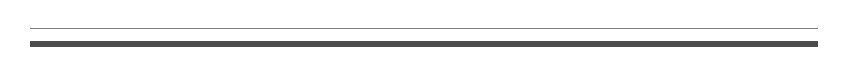
\begin{tikzpicture}
        \draw[line width=2pt, black!70] (0,0) -- (10,0);
        \draw[line width=0.5pt, black!50] (0,0.2) -- (10,0.2);
    \end{tikzpicture}
    
    \vspace{1cm}
    
    % Título principal
    {\fontsize{28}{34}\selectfont\bfseries 
    Análisis de Sistemas\\[0.3cm]
    Dinámicos y Estimación}
    
    \vspace{0.5cm}
    
    {\Large\textbf{EL3204-1}}
    
    \vspace{1cm}
    
    % Líneas decorativas inferiores
    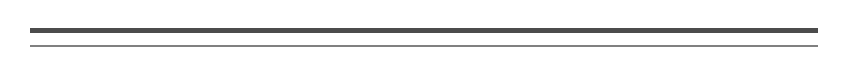
\begin{tikzpicture}
        \draw[line width=0.5pt, black!50] (0,0) -- (10,0);
        \draw[line width=2pt, black!70] (0,0.2) -- (10,0.2);
    \end{tikzpicture}
    
    \vspace{1.5cm}
    
    % Subtítulo
    {\LARGE\itshape Guía de Ejercicios Resueltos}
    
    \vspace{0.5cm}
    
    {\large Erik Sáez Aravena.}
    
    \vfill
    

    \vspace{1cm}
    
    % Decoración con ecuación diferencial de fondo
    \begin{tikzpicture}[remember picture, overlay]
        \node[opacity=0.08] at (current page.center) {
            \begin{tikzpicture}
                \node[font=\fontsize{120}{140}\selectfont, black!30] at (0,0) {$\dot{\mathbf{x}}$};
            \end{tikzpicture}
        };
    \end{tikzpicture}
    
    \vspace{1cm}
    
\end{center}
\clearpage

% ============================================
% CONTENIDO
% ============================================

\begin{questions}
    %%%%%%%%%%%%%%%%%%%%%%%%%%%
    \question Considere el sistema de la siguiente figura, donde se tiene un carro atado a un resorte con un sensor de distancia, capaz de medir la distancia del carro a la pared. Suponga que existe una fuerza de fricción viscosa con la superficie $F_f$ de la forma $F_f = b_1 \dot{z} + b_2 (\dot{z}^2)$.
    \begin{figure}[ht]
        \centering
        \includegraphics[width=0.45\textwidth]{Auxiliar_1_1}
    \end{figure}
    \begin{enumerate}
        \item Establezca hipótesis simplificatorias para el problema.
        \item Formule un modelo matemático del sistema que sea consistente con sus hipótesis.
        \item Encuentre el punto de operación que asegure $z = 1$ m.
    \end{enumerate}
    %%%%%%%%%%%%%%%%%%%%%%%%%%%
    \begin{solution}
    \subsection*{Resolución 1.1}
        Para poder plantear un buen modelo, es necesario establecer hipótesis que simplifiquen el problema y lo hagan abordable. Estas hipótesis son muy importantes, ya que pueden complejizar o simplificar el problema cuanto sea necesario. Para este caso particular, algunas hipótesis que se pueden plantear para simplificar el problema son:
\begin{enumerate}
    \item El carro solamente se mueve \textbf{horizontalmente.}
    \item El resorte actúa en el \textbf{régimen lineal}, de acuerdo a la ley de Hooke.
    \item La constante elástica $k$ del resorte no varía, y su largo natural $l_0$ es 0.
    \item La fricción es de la forma 
    \begin{equation}
        F_f = b_1 \dot{z} + b_2 \dot{z}^2.
    \end{equation}
    \item La fuerza $F(t)$ es conocida y varía en el tiempo.
\end{enumerate}
\subsection*{Resolución 1.2}
Plantear un modelo matemático para un sistema físico se reduce, generalmente, a encontrar una ecuación diferencial que modele la dinámica del sistema. Para este caso particular, podemos utilizar la segunda ley de Newton para obtener dicha ecuación diferencial (esto es una de las tantas formas posibles de abordar el problema).
\begin{equation}
    m\ddot{z} = F(t) - F_e - F_f, 
\end{equation}
Donde $F_e$ corresponde a la fuerza elástica del resorte y $F_f$ es la fuerza de fricción. La fuerza elástica, debido a la segunda hipótesis (\textit{$l_{0}=0$}), estará dada por:
\begin{equation}
    F_e = kz, 
\end{equation}
por lo que la ecuación anterior es
\begin{equation}
    m\ddot{z} = F(t) - kz - b_1\dot{z} - b_2\dot{z}^2. 
\end{equation}
Despejando $\ddot{z}$, tenemos que el modelo matemático es
\begin{equation}
    \ddot{z} = \frac{1}{m}F(t) - \frac{k}{m}z - \frac{b_1}{m}\dot{z} - \frac{b_2}{m}\dot{z}^2. 
\end{equation}
Sabemos que este será el modelo matemático, ya que captura la dinámica del sistema en función de las fuerzas actuantes y las propiedades del resorte. 
\subsection*{Resolución 1.3}
Para encontrar el punto de operación, el objetivo es determinar el valor de la entrada $F(t)$ de modo tal que se tenga $z = 1 \, \text{m}$. Implícitamente, al hablar de punto de operación se requiere estaticidad (a menos que se indique lo contrario), por lo que podemos asumir que $z$ no varía, indicando que $\dot{z} = \ddot{z} = 0$.

Podemos utilizar lo anteriormente mencionado sobre el modelo, imponiendo las condiciones indicadas y encontrando el valor de $F(t)$ que las satisfaga. Imponiendo $z = 1$, $\dot{z} = \ddot{z} = 0$ sobre la ecuación anterior, tenemos:
\begin{equation}
    0 = \frac{1}{m}F(t) - \frac{k}{m} \cdot 1 \quad \Rightarrow \quad F(t) = k,
\end{equation}
por lo que el punto de operación es $F(t) = k$. Un aspecto importante a considerar es que, para encontrar este punto de operación, asumimos que la fuerza $F(t)$ es constante en el tiempo. Más adelante en el curso (y en otros cursos de la carrera) veremos que considerar una fuerza constante no siempre es lo ideal, sino que es posible diseñar una entrada particular para alcanzar la condición de estaticidad más rápidamente.
    \end{solution}
    \newpage
    %%%%%%%%%%%%%%%%%%%%%%%%%%%
    \question Considere el siguiente péndulo apoyado en un carro móvil, el cual se desliza por una barra.
    \begin{enumerate}
        \item Establezca hipótesis simplificatorias.
        \item Formule un modelo matemático, que capture la dinámica del sistema.
        \item Identifique entradas, salidas y estados en su modelo.
        \item Linealice en torno a $\theta = \pi$.
    \end{enumerate}
    \begin{figure}[ht]
        \centering
        \includegraphics[width=0.5\textwidth]{Auxiliar_1_2}
    \end{figure}
%%%%%%%%%%%%%%%%%%%%%%%%%%%
\begin{solution}
\subsection*{Resolución 2.1}
    Primeramente, es necesario establecer buenas hipótesis simplificatorias para que el problema sea abordable. Algunas de estas hipótesis que podemos plantear son las siguientes:
\begin{enumerate}
    \item El carro tiene masa despreciable.
    \item La vara del péndulo no tiene masa.
    \item La vara del péndulo es rígida.
    \item La bola del péndulo es una masa puntual.
    \item No hay roce con el aire.
    \item Solamente existe movimiento en los dos ejes ilustrados.
\end{enumerate}
\subsection*{Resolución 2.2}
Utilizando las hipótesis planteadas, podemos encontrar un modelo matemático. Para esto, si bien se podría utilizar la segunda ley de Newton para plantear una ecuación diferencial, al ser un péndulo este es un proceso engorroso: en cambio, utilizaremos mecánica lagrangiana para plantear la ecuación diferencial. El lagrangiano corresponde a $L = T - V$, con $T$ la energía cinética y $V$ la energía potencial, junto a la ecuación de Euler-Lagrange
\begin{equation}
    \frac{\partial L}{\partial q} - \frac{d}{dt} \left( \frac{\partial L}{\partial \dot{q}} \right) = 0
\end{equation}
Es importante destacar que (\textbf{q}) representa la coordenada que estemos utilizando y por tanto dependerá también del sistema de coordenadas que se utilice. Además, la ecuación de Euler-Lagrange planteada de esa manera es válida si no existen pérdidas de energía en el sistema: si hubiesen fuerzas no conservativas, se deberían considerar dentro de la ecuación. Este supuesto es válido debido a la hipótesis de que no hay fricción. Para calcular el Lagrangiano, debemos comenzar calculando la energía cinética. Dado que solamente la bola del péndulo tiene masa, este será el único componente con energía cinética. Si llamamos $x_p, y_p$ a la posición del péndulo, podemos notar que esta se puede escribir como
\begin{equation}
    x_p = x + l \sin \theta \quad y_p = -l \cos \theta,
\end{equation}
Donde deberemos definir el sistema de referencia el cual se asume que $y$ es positivo hacia arriba, que $y = 0$ corresponde a la ubicación de la barra, y que se tiene una distancia $x(t)$ desde el origen a la vertical del péndulo. Con estas posiciones, la energía cinética estará dada por:
\begin{equation}
    T = \frac{1}{2} m \left( \dot{x}_p^2 + \dot{y}_p^2 \right). 
\end{equation}
 Dado que necesitamos las derivadas para el cálculo anterior, tenemos
\begin{equation}
    \dot{x}_p = \dot{x} + l \dot{\theta} \cos \theta \quad \dot{y}_p = l \dot{\theta} \sin \theta
\end{equation}
donde los términos $\dot{\theta}$ salen por la regla de la cadena (\textit{Es muy importante tener en consideración esto último, dado que $\dot{\theta}$ depende del tiempo, que es respecto a lo que estamos derivando}). Utilizándolos para calcular la energía cinética, tenemos:
\begin{equation}
    T = \frac{1}{2} m \left( \dot{x}^2 + 2 \dot{x} l \dot{\theta} \cos \theta + l^2 \dot{\theta}^2 \cos^2 \theta + l^2 \dot{\theta}^2 \sin^2 \theta \right)
\end{equation}
Podemos notar que:
\begin{equation}
    l^2 \dot{\theta}^2 \cos^2 \theta + l^2 \dot{\theta}^2 \sin^2 \theta = l^2 \dot{\theta}^2 (\cos^2 \theta + \sin^2 \theta) = l^2 \dot{\theta}^2
\end{equation}
Luego:
\begin{equation}
    T = \frac{1}{2} m \left( \dot{x}^2 + 2 \dot{x} l \dot{\theta} \cos \theta + l^2 \dot{\theta}^2 \right) = \frac{1}{2} m \dot{x}^2 + m l \dot{x} \dot{\theta} \cos \theta + \frac{1}{2} m l^2 \dot{\theta}^2. 
\end{equation}
Para la energía potencial, dado que el único componente que tiene masa es la bola del péndulo, solamente se tiene la contribución de su energía potencial gravitatoria. Además, dado que la vara es rígida, sabemos que no actúa como un resorte y, por ende, no hay energía potencial elástica. Considerando todo esto, la energía potencial $V$ está dada por
\begin{equation}
    V = mg \cdot y_p = -mgl \cos \theta. 
\end{equation}
Luego, el lagrangiano es
\begin{equation}
    L = \frac{1}{2} m \left( \dot{x}^2 + 2 \dot{x} l \dot{\theta} \cos \theta + l^2 \dot{\theta}^2 \right) + mgl \cos \theta. 
\end{equation}
Para poder considerar el Lagrangiano dentro de la ecuación de Euler-Lagrange, es necesario calcular las derivadas de cada término. Dado que estamos trabajando en coordenadas polares, sabemos que hay dos coordenadas, el radio \(r\) y el ángulo \(\theta\). Dado que \(r = l\) es constante, sabemos que no hay dinámica en la dirección radial, por lo que solamente nos interesa analizar la dinámica angular. Esto significa que debemos calcular las derivadas de \(L\) con respecto a \(\theta\) y \(\dot{\theta}\). Calculando las derivadas, tenemos
\begin{align}
    \frac{\partial L}{\partial \theta} &= -mgl \,\sin \theta \;-\; ml\,\dot{x}\,\dot{\theta}\,\sin \theta, \\
    \frac{\partial L}{\partial \dot{\theta}} &= ml^2\,\dot{\theta} \;+\; ml\,\dot{x}\,\cos \theta.
\end{align}
Un punto importante a notar a la hora de calcular las derivadas es que, al derivar respecto a $\theta$, se debe tener en cuenta que $\dot{\theta}$ no depende de $\theta$, sino solamente del tiempo. Lo mismo aplica a la hora de derivar respecto a $\dot{\theta}$, donde $\dot{\theta}$ actúa como una constante.
Luego, usando la ecuación 21 podemos tomar la derivada con respecto al tiempo, de lo que tenemos
\begin{align}
    \frac{d}{dt} \left( \frac{\partial L}{\partial \dot{\theta}} \right) 
    &= \frac{d}{dt} \left( ml^2 \dot{\theta} + ml \dot{x} \cos \theta \right) \tag{22}\\
    &= ml^2 \ddot{\theta} + ml \left( \ddot{x} \cos \theta - \dot{x} \dot{\theta} \sin \theta \right) \\
    &= ml^2 \ddot{\theta} + ml \ddot{x} \cos \theta - ml \dot{x} \dot{\theta} \sin \theta.
\end{align}
Insertando estos términos dentro de la ecuación de Euler--Lagrange, tenemos
\begin{align}
    \frac{\partial L}{\partial \theta} - \frac{d}{dt} \left( \frac{\partial L}{\partial \dot{\theta}} \right) &= 0 \\
    &= \left[ -mgl \sin \theta - ml\,\dot{x}\,\dot{\theta}\,\sin \theta \right] 
       - \left[ ml^2 \ddot{\theta} + ml\,\ddot{x} \cos \theta - ml\,\dot{x}\,\dot{\theta}\,\sin \theta \right] \\
    &= -mgl \sin \theta - ml^2 \ddot{\theta} - ml\,\ddot{x} \cos \theta = 0. 
\end{align}
Reordenando términos para despejar \(\ddot{\theta}\) en función del resto de variables, obtenemos
\begin{equation}
    \ddot{\theta} = -\frac{g}{l} \sin \theta - \frac{\cos \theta}{l} \,\ddot{x}, 
\end{equation}
la cual corresponde a la ecuación diferencial que modela la dinámica del problema.
\subsection*{Resolución 2.3}
Para identificar las entradas, debemos identificar aquellas variables que podemos manipular y que no dependen de la dinámica del problema. En este caso, podemos ver que $\ddot{x}$, correspondiente a la aceleración del carro, es una variable libre del problema, la cual no depende del resto de variables, por lo que podemos considerarla como la entrada al sistema.\\
Con respecto a la salida, esta es la variable que más libertad entrega a quien modela, dado que depende del fenómeno de interés. En general, se puede considerar como variable de salida cualquiera de los sensores que se están utilizando para medir las variables, por lo que estos valores medidos por los sensores podrían considerarse las salidas. Sin embargo, en este problema no se indican los sensores presentes, por lo que asumiremos que cualquier variable es salida, por lo que, arbitrariamente, se escoge que $\theta$ es la salida.\\
Finalmente, las últimas variables a indicar son los estados. Los estados corresponden a aquellas variables que tienen incidencia directa sobre la dinámica del sistema planteado. Una forma práctica de verlo es que cualquier diferencial que modele al sistema: si el sistema está modelado por una EDO de orden n, entonces todas las derivadas de menor orden (incluyendo el orden 0, que corresponde a la variable sin derivar) van a corresponder a los estados del sistema\footnote{Otra forma útil de verlo es que los estados van a corresponder a todas aquellas variables para las cuales se debe indicar una condición inicial.}. En el problema planteado, dado que el modelo es una EDO de orden 2, sabemos que las derivadas de orden 1 ($\dot{\theta}$) y orden 0 ($\theta$) serían los estados del sistema.
\subsection*{Resolución 2.4}
La linealización es un proceso en el cual generamos una aproximación lineal de la EDO que modela al sistema, utilizando los primeros términos de la serie de Taylor.
Para esto, notemos que podemos escribir la ecuación (29) como
\begin{equation}
    \ddot{\theta} = f(\theta, u),
\end{equation}
tal que
\begin{equation}
    f(\theta, u) = -\frac{g}{l} \sin \theta - \frac{\cos \theta}{l} u,
\end{equation}
donde hemos denotado $u = \ddot{x}$ para abreviar. 

La idea de linealizar es calcular la serie de Taylor de la función $f(\theta, u)$ en torno a un cierto punto $(\bar{\theta}, \bar{u})$, de modo que el sistema linealizado sea una \textbf{buena aproximación del sistema original en torno a dicho punto}.

Calculando la serie de Taylor de $f(\theta, u)$ en torno a $(\bar{\theta}, \bar{u})$ y omitiendo términos de orden superior, tenemos:
\begin{equation}
    f(\theta, u) \approx f(\bar{\theta}, \bar{u}) 
    + (\theta - \bar{\theta}) \frac{\partial f(\bar{\theta}, \bar{u})}{\partial \theta} 
    + (u - \bar{u}) \frac{\partial f(\bar{\theta}, \bar{u})}{\partial u}.
\end{equation}

Definimos las variables perturbadas:
\begin{equation}
    \tilde{\theta} := \theta - \bar{\theta}, 
    \qquad 
    \tilde{u} := u - \bar{u},
\end{equation}
y considerando que $\ddot{\theta} = f(\theta, u)$ y $\tilde{\ddot{\theta}} := \ddot{\theta} - f(\bar{\theta}, \bar{u})$, obtenemos:
\begin{equation}
    \tilde{\ddot{\theta}} = f_{\theta}(\bar{\theta}, \bar{u}) \, \tilde{\theta} 
    + f_{u}(\bar{\theta}, \bar{u}) \, \tilde{u}.
\end{equation}

Donde, para abreviar, definimos:
\begin{align}
    f_{\theta} &:= \frac{\partial f(\bar{\theta}, \bar{u})}{\partial \theta} 
    = -\frac{g}{l} \cos \bar{\theta} + \frac{\sin \bar{\theta}}{l} \, \bar{u}, \\
    f_{u} &:= \frac{\partial f(\bar{\theta}, \bar{u})}{\partial u} 
    = -\frac{\cos \bar{\theta}}{l}.
\end{align}

Evaluando en $(\bar{\theta}, \bar{u}) = (\pi, 0)$:
\begin{align}
    f_{\theta}(\pi, 0) &= -\frac{g}{l} \cos \pi + \frac{\sin \pi}{l} \cdot 0 
    = -\frac{g}{l}(-1) + 0 
    = \frac{g}{l}, \\
    f_{u}(\pi, 0) &= -\frac{\cos \pi}{l} 
    = -\frac{-1}{l} 
    = \frac{1}{l}.
\end{align}

Por lo tanto, el modelo linealizado en torno a \(\theta = \pi\) y \(u = 0\) es:
\begin{equation}
    \tilde{\ddot{\theta}} = \frac{g}{l} \, \tilde{\theta} + \frac{1}{l} \, \tilde{u}.
\end{equation}
Con lo que finalmente se obtiene el modelo linealizado.
\end{solution}
\newpage
%%%%%%%%%%%%%%%%%%%%%%%%%%%
\question Considere el siguiente estanque cónico:
\begin{figure}[ht]
    \centering
    \includegraphics[width=0.4\textwidth]{Auxiliar_1_5}
    \caption{Estanque cónico}
\end{figure}

Se tienen los siguientes datos:
\begin{itemize}
    \item Altura máxima: $H = 8 \, \text{m}$
    \item Radio máximo: $R = 3 \, \text{m}$
    \item Volumen del estanque en función de la altura:
    \begin{equation}
        V(h) = \frac{\pi r^2 h}{3}, \tag{1}
    \end{equation}
    \item Flujo volumétrico de entrada: $F_1(t)$ (arbitrario)
    \item Flujo volumétrico de salida:
    \begin{equation}
        F(t) = \alpha \sqrt{h(t)}
    \end{equation}
    donde $\alpha$ corresponde a la apertura del canal. Para este ejercicio, considere $\alpha = 1$.
\end{itemize}

Responda lo siguiente:
\begin{enumerate}
    \item Encuentre un modelo dinámico no lineal que relacione la altura del agua $h(t)$ y el flujo de entrada $F_1(t)$, indicando claramente las hipótesis simplificatorias que tome.

    \item Linealice su modelo en torno a $h_0 = 4\,\text{m}$, $F_{1,0} = 2\,\text{m}^3/\text{s}$, y plantee una nueva ecuación diferencial lineal para el modelo perturbado, considerando:
    \begin{align*}
        h(t) &= h_0 + \Delta h(t) \\
        F_1(t) &= F_{1,0} + \Delta F_1(t)
    \end{align*}
    que relacione la salida del sistema linealizado $\Delta h(t)$ con la entrada del sistema linealizado $\Delta F_1(t)$. Para esto, al linealizar puede considerar que los términos de orden superior (por ejemplo, $\Delta h^2$, $\Delta F_1^2$, etc.) son despreciables y pueden anularse.
\end{enumerate}
%%%%%%%%%%%%%%%%
\begin{solution}
\subsection*{Resolución 3.1}
Dado que se busca plantear un modelo dinámico no lineal, es necesario establecer hipótesis simplificatorias adecuadas. Algunas que podemos considerar son las siguientes:
\begin{itemize}
    \item El estanque es un cono perfecto.
    \item No existen pérdidas de agua ni entradas adicionales al sistema.
    \item La velocidad del agua es lo suficientemente baja como para despreciar efectos inerciales.
    \item La superficie libre del agua es plana en todo momento.
    \item \ldots
\end{itemize}

La variación del volumen de agua en el estanque está determinada por la diferencia entre el flujo volumétrico de entrada y el flujo volumétrico de salida:
\begin{equation}
    \frac{dV}{dt} = F_1(t) - F(t).
\end{equation}

Recordando que el volumen de un cono está dado por:
\begin{equation}
    V(h) = \frac{\pi r^2 h}{3},
\end{equation}
observamos que el radio \(r(t)\) también depende del tiempo. Para relacionar \(r(t)\) con \(h(t)\) utilizamos el Teorema de Tales, considerando la geometría del estanque:

\begin{center}
    \includegraphics[width=0.2\textwidth]{Auxiliar_1_6}
\end{center}

De este modo:
\begin{align}
    \frac{r(t)}{h(t)} = \frac{R}{H} 
    \quad \Rightarrow \quad 
    r(t) = \frac{R}{H} \, h(t).
\end{align}

Sustituyendo en la expresión del volumen, se obtiene:
\begin{align}
    V(h) &= \frac{\pi \left( \frac{R}{H} h \right)^2 h}{3} 
    = \frac{\pi R^2}{3 H^2} h^3.
\end{align}

Derivando respecto del tiempo y usando la ecuación de balance de volúmenes:
\begin{align}
    \frac{dV}{dt} &= F_1(t) - F(t) \\
    \frac{d}{dt} \left( \frac{\pi R^2}{3 H^2} h^3 \right) = F_1(t) - F(t), \\
    \frac{\pi R^2}{H^2} h^2 \dot{h} &= F_1(t) - F(t).
\end{align}

Definiendo:
\begin{equation}
    k := \frac{\pi R^2}{H^2},
\end{equation}
y considerando que el flujo de salida está dado por \(F(t) = \alpha \sqrt{h(t)}\), se obtiene:
\begin{align}
    \dot{h} = \frac{1}{k\, h^{2}} \left[ F_1(t) - \alpha \sqrt{h(t)} \right].
\end{align}

Se observa que este modelo es claramente no lineal, ya que la ecuación diferencial contiene términos $\frac{1}{h^2}$ y $\sqrt{h}$.

   \subsection*{Resolución 3.2}
Se comienza considerando el modelo no lineal obtenido anteriormente:
\begin{equation}
    \dot h \;=\; f(h,F_1) \;=\; \frac{F_1 - \sqrt{h}}{k\,h^2},
    \qquad k := \frac{\pi R^2}{H^2},
\end{equation}
con el punto de operación dado por el enunciado:
\begin{equation}
    h_0 = 4\,\text{m}, 
    \qquad F_{1,0} = 2\,\text{m}^3/\text{s},
    \qquad \alpha=1,
\end{equation}
el cual satisface $0 = \frac{F_{1,0}-\sqrt{h_0}}{k h_0^2}$ (i.e., $F_{1,0}=\sqrt{h_0}=2$). Con lo que sabemos que es un punto de equilibrio. Luego se definen las perturbaciones:
\begin{equation}
    \Delta h := h - h_0,
    \qquad
    \Delta F_1 := F_1 - F_{1,0},
    \qquad
    \Delta \dot h := \dot h - \dot h_0 =\dot h.
\end{equation}

Linealizamos por serie de Taylor de $f(h,F_1)$ en $(h_0,F_{1,0})$:
\begin{equation}
    \Delta \dot h 
    \;=\; 
    \left.\frac{\partial f}{\partial h}\right|_{0}\,\Delta h
    \;+\;
    \left.\frac{\partial f}{\partial F_1}\right|_{0}\,\Delta F_1 .
\end{equation}
Sea $f(h,F_1) = \dfrac{F_1 - \sqrt{h}}{k\,h^2}$. Entonces
\begin{align}
    \frac{\partial f}{\partial h}
    &= \frac{1}{k}\,\frac{\partial}{\partial h}\!\left[(F_1-\sqrt{h})\,h^{-2}\right] \nonumber\\
    &= \frac{1}{k}\left[ -\frac{1}{2}h^{-1/2}\,h^{-2} \;+\; (F_1-\sqrt{h})(-2)h^{-3}\right],\\[0.25em]
    \frac{\partial f}{\partial F_1}
    &= \frac{1}{k}\,h^{-2}.
\end{align}
Evaluando en el punto de operación $(h_0,F_{1,0})=(4,2)$ (nótese que $F_{1,0}-\sqrt{h_0}=0$):
\begin{align}
    \left.\frac{\partial f}{\partial h}\right|_0
    &= \frac{1}{k}\left[-\frac{1}{2}h_0^{-5/2}\right]
    \;=\; -\frac{1}{2k}\,(4)^{-5/2}
    \;=\; -\frac{1}{64k},\\
    \left.\frac{\partial f}{\partial F_1}\right|_0
    &= \frac{1}{k}\,h_0^{-2}
    \;=\; \frac{1}{16k}.
\end{align}

Por lo tanto, el modelo linealizado queda tal que:
\begin{equation}
    \boxed{\,\Delta \dot h \;=\; -\frac{1}{64k}\,\Delta h \;+\; \frac{1}{16k}\,\Delta F_1\,}
\end{equation}
Con $R=3\,\mathrm{m},\ H=8\,\mathrm{m}$. Aquí $k=\dfrac{\pi R^2}{H^2}=\dfrac{9\pi}{64}$. Reemplazando:
\begin{align}
    -\frac{1}{64k} &= -\frac{1}{64\cdot (9\pi/64)} \;=\; -\frac{1}{9\pi},\\
     \frac{1}{16k} &= \frac{1}{16\cdot (9\pi/64)} \;=\; \frac{4}{9\pi}.
\end{align}
Así,
\begin{equation}
    \boxed{\,\Delta \dot h \;=\; -\frac{1}{9\pi}\,\Delta h \;+\; \frac{4}{9\pi}\,\Delta F_1\,}
\end{equation}


\end{solution}

% =============================
% Preguntas del Auxiliar 2
% =============================
\newpage
\question Considere el siguiente circuito eléctrico, donde $\alpha(t)i_2(t)$ corresponde al valor de la resistencia eléctrica de un potenciómetro, cuyo valor depende tanto de $\alpha(t)$ como de la corriente que circula por el condensador, y $v_{out}(t)$ (voltaje en el condensador) se mide con un voltímetro.
\begin{figure}[ht]
    \centering
    \includegraphics[width=0.6\textwidth]{Auxiliar_2_1}
\end{figure}
\begin{enumerate}
    \item Establezca claramente el listado de hipótesis simplificatorias que permitan establecer un modelo matemático válido para este sistema. Indique las condiciones de borde y/o iniciales necesarias.
    \item Formule un modelo para el sistema en ecuaciones de estado.
    \item Caracterice completamente el modelo utilizando todos los puntos de vista descritos en clases. Clasifique todas las variables del sistema.
    \item Encuentre estado(s) cero, estado(s) de equilibrio y el estado tierra (de existir).
    \item Linealice el sistema en torno al (los) estado(s) de equilibrio encontrados.
\end{enumerate}
\begin{solution}
\subsection*{Resolución 4.1}
Para poder formular un modelo del sistema, debemos primeramente considerar hipótesis simplificatorias que permitan simplificar el problema o establecer límites sobre las distintas restricciones del mismo; por lo tanto:
\begin{itemize}
    \item Los parámetros $V_{in},\,R,\,R_0,\,C$ son constantes del sistema.
    \item El circuito opera en régimen de parámetros concentrados.
    \item Se desprecia la resistencia interna del voltímetro.
    \item No se consideran efectos parásitos ni ruidos.
    \item $\ldots$
\end{itemize}
Por otra parte, por conocimiento de circuitos se sabe que la condición inicial necesaria para determinar el estado del sistema corresponde al voltaje inicial del condensador $v_c(0)$.
\subsection*{Resolución 4.2}
Primero se aplica la Ley de Corrientes de Kirchhoff (LCK) en el nodo superior, con lo que se tiene $I(t)=i_1(t)+i_2(t)$. Además, utilizando la Ley de Voltajes de Kirchhoff (LVK) en la malla izquierda, se obtiene:
\begin{align}
V_{in}=RI+v_c = R i_1 + R i_2 + v_c .
\end{align}
Recordando la ecuación del condensador, $i_C=C\,\dot{v}_c$, e identificando $i_C=i_2$,
\begin{align}
V_{in}=R i_1 + RC\,\dot{v}_c + v_c .
\end{align}
En la rama de la derecha luego se tiene:
\begin{align}
v_c = R_0 i_1 + (\alpha\, i_2) i_1
    = R_0 i_1 + \alpha C \dot{v}_c\, i_1
    = \bigl(R_0 + \alpha C \dot{v}_c \bigr) i_1,
\end{align}
Despejando,
\begin{align}
i_1=\frac{v_c}{R_0+\alpha C \dot{v}_c}.
\end{align}
Sustituyendo la ecuación~(4) en la ecuación~(2) con el propósito de expresar todo en función de una única variable $v_{c}$, se llega a:
\begin{align}
V_{in}= \frac{R\,v_c}{R_0+\alpha C \dot{v}_c} + RC\,\dot{v}_c + v_c .
\end{align}
Reordenando y desarrollando,
\begin{align}
R_0 V_{in}+ \alpha C V_{in}\dot{v}_c
= Rv_c + R_0 RC \dot{v}_c + \alpha RC^2 \dot{v}_c^{\,2} + R_0 v_c + \alpha C v_c \dot{v}_c ,
\end{align}
lo que lleva a la ecuación cuadrática en $\dot{v}_c$:
\begin{align}
\alpha RC^2 \dot{v}_c^{\,2} + \bigl(R_0RC + \alpha C (v_c - V_{in})\bigr)\dot{v}_c
+ (R+R_0) v_c - R_0 V_{in} = 0.
\end{align}
Resolviendo para $\dot{v}_c$,
\begin{align}
\dot{v}_c
= \frac{-\bigl(R_0RC + \alpha C (v_c - V_{in})\bigr) \pm \sqrt{S}}
       {2\alpha RC^2},
\end{align}
donde, por conveniencia,
\begin{align}
S
&= R_0^2 R^2 C^2
+ 2\alpha R_0 R C^2 (v_c - V_{in})
+ \alpha^2 C^2 (v_c - V_{in})^2 \nonumber\\
&\quad - 4\alpha R C^2 (R+R_0) v_c
+ 4 R_0 R C^2 V_{in}.
\end{align}
Con lo que se obtiene finalmente la ecuación diferencial que caracteriza el sistema, la cual es evidentemente no lineal.
\subsection*{Resolución 4.3}
Existen diversas características con las que podemos clasificar los modelos, algunas de estas son las siguientes:
\begin{center}
\begin{tabular}{|p{3cm}|p{11cm}|}
\hline
Característica & Clasificación \\
\hline
Origen & Fenómeno artificial (sistema eléctrico construido). \\
\hline
Naturaleza & Determinístico (no se consideran ruidos $w(t)$ o $v(t)$). \\
\hline
Número de variables & Monovariable (un estado). \\
\hline
Continuidad & Continuo (aparece $\dot{v}_c$). \\
\hline
Comportamiento espacial & Parámetros concentrados. \\
\hline
Comportamiento temporal & Invariante en el tiempo. \\
\hline
Linealidad & No lineal (por la dependencia racional en $\dot{v}_c$). \\
\hline
Realizabilidad & Causal y realizable. \\
\hline
\end{tabular}
\end{center}

Además, deberemos definir las variables del sistema, las cuales se pueden definir de la siguiente manera:
\begin{itemize}
    \item Estado: $x(t)=v_c(t)$.
    \item Salida: $y(t)=v_{out}(t)=v_c(t)=x(t)$.
    \item Entrada: $u(t)=\alpha(t)$.
\end{itemize}
\subsection*{Resolución 4.4}
A continuación se analizan los diferentes estados del sistema:

\begin{itemize}
  \item Estado cero. Un estado cero $x_0 \in \Sigma$ es aquel tal que, $\forall$ $t_0$, la salida instantánea bajo entrada nula satisface
  \begin{equation*}
    \forall\, t_0:\; y(t_0) \,=\, \overline{A}(x_0,0) \,=\, 0.
  \end{equation*}
  Esta definición es atemporal: se refiere a una propiedad puntual de la relación estado–salida y no a la evolución posterior en el tiempo.
  En este sistema en particular, como $y=v_C=x$, el estado cero es $x_0 = 0$.

    \item Estado de equilibrio. Recordemos que un estado de equilibrio $x_e \in \Sigma$ es tal que $x_e = \overline{B}(x_e, 0)$. Esto significa que bajo entrada cero, lo que implica que $\alpha=0$, si el sistema está en estado de equilibrio, entonces permanecerá en este estado por siempre. Para encontrarlo, buscamos $x_e$ tal que $\dot{x}=0$. Evaluando esta condición en la ecuación cuadrática se obtiene:
    \begin{center}
        \includegraphics[width=0.6\textwidth]{Auxiliar_2_2}
    \end{center}
    Con lo que analizando la malla tenemos:
    \begin{align}
        V_{in} &= IR + R_{0}i_{1}\\
                &= i_{1}R + i_{2}R + R_{0}i_{1}\\
                &= (R + R_0)i_{1} + i_{2}R\\
                &=(R + R_0)i_{1} + RC\dot{v_{c}}\\
                &= (R + R_0)i_{1}
    \end{align}
    Anteriormente teníamos que $i_{1} = \frac{v_{c}}{R_{0}+\alpha C \dot{v_{c}}}$ y dado que $\alpha=\dot{v}_{c}=0$, por otro lado tendremos que el estado de equilibrio será $x_e = v_c$, podemos escribir
    \begin{align}
    (R+R_0)\,x_e - R_0 V_{in}=0 \quad \Rightarrow \quad
    x_e = \frac{R_0}{R+R_0}\,V_{in}.
    \end{align}
    
    \item Estado tierra. Recordemos que un estado tierra $x_t \in \Sigma$ de un sistema es tal que $\forall x_0 \in \Sigma, \lim_{t \to \infty} \overline{B}(x_0, 0) = x_t$. El estado tierra es aquel al cual converge el sistema para toda condición inicial y con entrada cero. Cuando el condensador está completamente cargado (en tiempo suficientemente grande), no conduce corriente y el circuito equivale a un divisor de tensión. Por lo tanto,
    \begin{align}
    x_t = \frac{R_0}{R+R_0}\,V_{in}.
    \end{align}
\end{itemize}
\subsection*{Resolución 4.5}
Buscamos linealizar el sistema con el motivo de obtener un modelo más simple que capture la dinámica del sistema cerca de algún punto de operación. 

\begin{align}
\dot{\tilde{x}} &= 
\left.\frac{\partial f}{\partial x}\right|_{\bar{x},\bar{u}} \tilde{x} 
+ \left.\frac{\partial f}{\partial u}\right|_{\bar{x},\bar{u}} \tilde{u}, \\[6pt]
\tilde{y} &= 
\left.\frac{\partial g}{\partial x}\right|_{\bar{x},\bar{u}} \tilde{x} 
+ \left.\frac{\partial g}{\partial u}\right|_{\bar{x},\bar{u}} \tilde{u}.
\end{align}

Donde tenemos que diferenciar correctamente que:
\begin{align}
    x &\coloneqq \text{Estado}\\
    \bar{x} &\coloneqq \text{Estado de operación}\\
    \tilde{x} &\coloneqq \text{Perturbación}
\end{align} 

Lo mismo aplica para $u$. Luego podemos definir la relación entrada-salida del sistema como $f(x,u) = f(v_{c},\alpha)$ y $g(x,u) = g(v_{c},\alpha)$. 

Considerando el punto de operación $\bar{v}_c = \frac{R_0}{R + R_0} V_{in}$ y $\bar{\alpha} = 1$, y tras calcular las derivadas parciales correspondientes y evaluarlas en el punto de operación, obtenemos el sistema linealizado:

\begin{align}
\dot{\tilde{x}} &= A\tilde{x} + B\tilde{u}\\
\tilde{y} &= \tilde{x} 
\end{align}

donde $A$ y $B$ son las matrices del sistema linealizado que dependen de los parámetros del circuito evaluados en el punto de operación.
\end{solution}
\newpage
\question Considere el sistema linealizado del auxiliar anterior, modelado por la siguiente ecuación diferencial:
\begin{equation}
    \ddot{\theta}(t) = \frac{g}{l} \theta(t) + \frac{1}{l} u(t)
\end{equation}
\begin{enumerate}
    \item Descomponer la salida como la suma de la respuesta a condiciones iniciales nulas y la respuesta a entrada nula en el dominio de Laplace.
    \item Obtener la función de transferencia del sistema y encontrar la respuesta al impulso con condiciones iniciales nulas en el dominio del tiempo.
    \item Obtener la respuesta a entrada nula en el dominio del tiempo, y expresar la respuesta para una entrada y condiciones iniciales arbitrarias.
    \item Encuentre la salida cuando la entrada es un escalón unitario.
\end{enumerate}
\begin{solution}
\subsection*{Resolución 5.1}
Para realizar la descomposición, trabajemos en el dominio de Laplace debido a que dicho dominio facilita el análisis de sistemas lineales. Aplicando la transformada de Laplace sobre la ecuación diferencial del sistema, se tiene:
\begin{equation}
\mathcal{L}\left\{ \ddot{\theta} \right\} = s^2\Theta(s) - s\theta(0) - \dot{\theta}(0),
\end{equation}
donde los términos $\theta(0)$ y $\dot{\theta}(0)$ representan las condiciones iniciales del sistema. A continuación:
\begin{equation}
s^2\Theta(s) - s\theta(0) - \dot{\theta}(0) = \frac{g}{l} \Theta(s) + \frac{1}{l} U(s).
\end{equation}

Reordenando para despejar el término de la salida, tenemos:
\begin{equation}
\Theta(s) = \frac{s\theta(0) + \dot{\theta}(0)}{s^2 - \frac{g}{l}} + \frac{1}{l} \frac{1}{s^2 - \frac{g}{l}} U(s),
\end{equation}

donde podemos ver que la salida $\Theta(s)$ está escrita como la suma de dos términos. El primero de ellos corresponde a la salida cuando se tienen condiciones iniciales arbitrarias pero entrada nula, denominada RENC (Respuesta a Entrada Nula o Cero). El segundo término corresponde a la salida cuando utilizamos condiciones iniciales nulas pero una entrada arbitraria, denominada RESC (Respuesta a Estado Cero).

\subsection*{Resolución 5.2}
La noción de función de transferencia está estrechamente ligada con la RESC, ya que para obtener la función de transferencia, asumimos condiciones iniciales nulas y una entrada arbitraria. La función de transferencia $H(s)$ del sistema se define como:
\begin{equation}
H(s) = \frac{\Theta_s(s)}{U(s)} = \frac{1}{l} \frac{1}{s^2 - \frac{g}{l}}.
\end{equation}

Definiendo $\omega_0 := \sqrt{\frac{g}{l}}$, tenemos
\begin{equation}
H(s) = \frac{1}{l} \frac{1}{(s - \omega_0)(s + \omega_0)}.
\end{equation}

Para obtener la respuesta al impulso, aplicamos descomposición en fracciones parciales y luego la transformada inversa de Laplace:
\begin{align}
    H(s) &= \frac{1}{2\omega_0 l} \left( \frac{1}{s - \omega_0} - \frac{1}{s + \omega_0} \right)\\
    h(t) &= \mathcal{L}^{-1}\left\{ H(s) \right\} = \frac{1}{2\omega_0 l} \left( e^{\omega_0 t} - e^{-\omega_0 t} \right) = \frac{1}{\omega_0 l} \sinh(\omega_0 t).
\end{align}

\subsection*{Resolución 5.3}
Para obtener la RENC (Respuesta a Entrada Nula), aplicamos descomposición en fracciones parciales a:
\begin{equation}
\Theta_0(s) = \frac{s\theta(0) + \dot{\theta}(0)}{(s - \omega_0)(s + \omega_0)}.
\end{equation}

Resolviendo el sistema de ecuaciones para las constantes de fracciones parciales, obtenemos:
\begin{equation}
\theta_0(t) = \frac{\omega_0\theta(0) + \dot{\theta}(0)}{2\omega_0} e^{\omega_0 t} + \frac{\omega_0\theta(0) - \dot{\theta}(0)}{2\omega_0} e^{-\omega_0 t}.
\end{equation}

La respuesta completa del sistema ante condiciones iniciales y entrada arbitrarias es:
\begin{equation}
\theta(t) = \frac{\omega_0\theta(0) + \dot{\theta}(0)}{2\omega_0} e^{\omega_0 t} + \frac{\omega_0\theta(0) - \dot{\theta}(0)}{2\omega_0} e^{-\omega_0 t} + \frac{1}{\omega_0 l} \sinh(\omega_0 t) \ast u(t).
\end{equation}

\subsection*{Resolución 5.4}
Para encontrar la salida cuando la entrada es un escalón unitario, asumimos condiciones iniciales nulas y $u(t) = u_0(t)$. La transformada de Laplace del escalón unitario es $U(s) = \frac{1}{s}$, por lo que:
\begin{equation}
\Theta(s) = H(s) U(s) = \frac{1}{l} \frac{1}{s(s^2 - \omega_0^2)}.
\end{equation}

Aplicando fracciones parciales y la transformada inversa de Laplace, tenemos:
\begin{equation}
\theta(t) = \frac{1}{l\omega_0^2} \left( \cosh(\omega_0 t) - 1 \right).
\end{equation}
\end{solution}

\newpage

  \question Considere un sistema modelado por la siguiente ecuación diferencial:
  \begin{equation}
    \ddot y + 2\dot y - 15 y = u.
  \end{equation}

  \begin{parts}
    \part Encuentre la función de transferencia del sistema.
    \part Formule el sistema en variables de estado.
    \part Obtenga la MTE del sistema y encuentre las funciones base.
    \part Encuentre la respuesta al impulso del sistema.
    \part Determine la estabilidad BIBS y BIBO del sistema.
  \end{parts}
%----------------------------------
\begin{solution}
  \subsection*{Resolución 1.1}
  Recordemos que la función de transferencia relaciona la entrada y la salida de un sistema. Es útil trabajar en el dominio de Laplace dado que simplifica los cálculos. Definimos \(H(s)\) tal que
  \begin{equation}
    H(s) = \frac{Y(s)}{U(s)}.
  \end{equation}
 Dado que nuestro sistema es una ecuacion diferencial en el dominio temporal, deberemos aplicar la transformada de Laplace. Ademas tenemos que tener en consideracion condiciones iniciales nulas (consideramos la respuesta de estado cero). Utilizando la siguiente expresion:
 \begin{equation}
   \mathcal{L}\{\dot{y}\} = sY(s) - y(0),
 \end{equation}
  y, en general, para la $n$-ésima derivada se cumple
  \begin{equation}
    \mathcal{L}\{y^{(n)}(t)\}
    = s^{n} Y(s) - s^{n-1} y(0) - s^{n-2} \dot y(0) - \cdots - y^{(n-1)}(0),
  \end{equation}
  Para la ecuación diferencial dada, aplicando la transformada de Laplace y considerando condiciones iniciales nulas, tenemos
  \begin{equation}
    \mathcal{L}\{\ddot y + 2\dot y - 15 y\}
    = s^{2}Y(s) + 2sY(s) - 15Y(s) = U(s).
  \end{equation}
  Reordenando,
  \begin{equation}
    H(s) = \frac{Y(s)}{U(s)} = \frac{1}{s^{2} + 2s - 15}
    = \frac{1}{(s+5)(s-3)}.
  \end{equation}
  \subsection*{Resolución 1.2}
Para hacer la formulación en variables de estado, utilizaremos dos métodos distintos, cada uno con sus ventajas y desventajas.

\paragraph{Método 1}
Este primer método permite, de forma relativamente directa, obtener una formulación en variables de estado a partir de la ecuación diferencial. En la ecuación diferencial que modela al sistema, si definimos $x_1 = y$ y $x_2 = \dot{y}$, notemos que tenemos de la ecuacion diferencial original
\begin{equation}
  \ddot{y} + 2\dot{y} - 15 y = u,
\end{equation}
Ahora tenemos que,
\begin{equation}
\dot{x}_2 + 2x_2 - 15x_1 = u \;\Leftrightarrow\; \dot{x}_2 = 15x_1 - 2x_2 + u,
\end{equation}
lo cual corresponde a la ecuación diferencial del segundo estado ($x_2$). Para obtener la ecuación diferencial asociada a $x_1$, notemos que, por la forma en que están definidos los estados, se tiene $\dot{x}_1 = x_2$, por lo que el par de ecuaciones diferenciales puede escribirse como
\begin{equation}
\begin{gathered}
\dot{x}_1 = x_2 \\
\dot{x}_2 = 15x_1 - 2x_2 + u
\end{gathered}
\;\;\Leftrightarrow\;\;
\frac{d}{dt}\begin{pmatrix} x_1 \\ x_2 \end{pmatrix}
=
\begin{pmatrix} 0 & 1 \\[2pt] 15 & -2 \end{pmatrix}
\begin{pmatrix} x_1 \\ x_2 \end{pmatrix}
+
\begin{pmatrix} 0 \\ 1 \end{pmatrix} u,
\end{equation}
lo cual, junto con el hecho de que
\begin{equation}
y = x_1 = \begin{pmatrix} 1 & 0 \end{pmatrix} \begin{pmatrix} x_1 \\ x_2 \end{pmatrix},
\end{equation}
Corresponde finalmente al sistema formulado en variables de estado.

\paragraph{Método 2}
Este método requiere más trabajo para obtener el sistema formulado en variables de estado, pero su ventaja es que reduce bastante trabajo en las siguientes partes. Este método se basa en que, si consideramos un sistema LTI arbitrario de la forma
\begin{equation}
\dot{x} = A x + B u
\end{equation}
\begin{equation}
y = C x,
\end{equation}
y le aplicamos la transformada de Laplace y reordenamos términos, se verifica que este sistema, en el dominio de Laplace, corresponde a
\begin{equation}
X(s) = (sI - A)^{-1} B\, U(s)
\end{equation}
\begin{equation}
Y(s) = C X(s).
\end{equation}

Así, para encontrar la formulación en variables de estado, podemos manipular los términos en el dominio de Laplace para encontrar $A$, $B$ y $C$ tales que el sistema tenga la forma deseada. Para esto, utilizaremos la función de transferencia, por lo que comenzaremos descomponiéndola en fracciones parciales.

Notemos que el denominador de la función de transferencia se puede factorizar como $s^2 + 2s - 15 = (s-3)(s+5)$, por lo que tenemos
\begin{equation}
H(s) = \frac{1}{(s-3)(s+5)}.
\end{equation}
Luego, queremos encontrar $\alpha$ y $\beta$ tales que
\begin{equation}
H(s) = \frac{\alpha}{s-3} + \frac{\beta}{s+5},
\end{equation}
donde, utilizando el método visto en auxiliares anteriores, se tiene
\begin{align}
  \frac{\alpha(s+5) + \beta(s-3)}{(s-3)(s+5)} &= \frac{1}{(s-3)(s+5)}
\end{align}
Por lo que se formula un sistema de ecuaciones dado por:
\begin{align}
  \alpha s + 5\alpha + \beta s - 3\beta &= 1\\
  s(\alpha + \beta) + (5\alpha - 3\beta) &= 1
\end{align}
Con lo que :
\begin{align}
  \alpha + \beta &= 0 \\
  5\alpha - 3\beta &= 1 \\
  \rightarrow
  \alpha = \frac{1}{8}, \quad \beta = -\frac{1}{8}
\end{align}


Como $H(s) = \dfrac{Y(s)}{U(s)}$ por definición, se tiene
\begin{equation}
Y(s) = \frac{1}{8}\,\frac{U(s)}{s-3} - \frac{1}{8}\,\frac{U(s)}{s+5}.
\end{equation}
La idea detrás de este método está en notar que esta expresión puede escribirse, de forma equivalente, como
\begin{equation}
Y(s) = \begin{pmatrix} \dfrac{1}{8} & -\dfrac{1}{8} \end{pmatrix}
\begin{pmatrix}
\dfrac{U(s)}{s-3} \\[8pt]
\dfrac{U(s)}{s+5}
\end{pmatrix}.
\end{equation}

El motivo de esta reescritura es que, como puede notarse, hemos expresado la salida de forma análoga a la relación $Y(s)=C\,X(s)$, considerando
\begin{equation}
C = \begin{pmatrix} \dfrac{1}{8} & -\dfrac{1}{8} \end{pmatrix}
\qquad
X(s) =
\begin{pmatrix}
\dfrac{U(s)}{s-3} \\[8pt]
\dfrac{U(s)}{s+5}
\end{pmatrix},
\end{equation}
por lo que ya tenemos uno de los términos ($C$). Luego, para obtener $A$ y $B$, notemos que
\begin{equation}
X(s) =
\begin{pmatrix}
X_1(s) \\ X_2(s)
\end{pmatrix}
=
\begin{pmatrix}
\dfrac{U(s)}{s-3} \\[8pt]
\dfrac{U(s)}{s+5}
\end{pmatrix},
\end{equation}
por lo que, analizando la primera ecuación, tenemos
\begin{equation}
X_1(s) = \frac{U(s)}{s-3}.
\end{equation}
Si reordenamos los términos, tenemos
\begin{equation}
s\,X_1(s) - 3\,X_1(s) = U(s),
\end{equation}
y, aplicando transformada inversa (suponiendo $x_1(0)=0$), notando que $sX_1(s)$ corresponde a la derivada de $x_1$, tenemos
\begin{equation}
\dot{x}_1 - 3x_1 = u \;\Leftrightarrow\; \dot{x}_1 = 3x_1 + u.
\end{equation}
Haciendo este mismo procedimiento para la segunda ecuación, se obtiene
\begin{equation}
\dot{x}_2 = -5x_2 + u,
\end{equation}
por lo que, juntando ambas ecuaciones diferenciales y añadiendo la expresión para la salida, tenemos
\begin{equation}
\frac{d}{dt}\begin{pmatrix} x_1 \\ x_2 \end{pmatrix}
=
\begin{pmatrix} 3 & 0 \\[2pt] 0 & -5 \end{pmatrix}
\begin{pmatrix} x_1 \\ x_2 \end{pmatrix}
+
\begin{pmatrix} 1 \\ 1 \end{pmatrix} u
\end{equation}
\begin{equation}
y = \begin{pmatrix} \dfrac{1}{8} & -\dfrac{1}{8} \end{pmatrix}
\begin{pmatrix} x_1 \\ x_2 \end{pmatrix},
\end{equation}
lo cual corresponde al sistema formulado en variables de estado. Si bien este procedimiento requiere más trabajo que el anterior, el sistema resultante tiene una ventaja clave: la matriz $A$ queda diagonal, a diferencia del obtenido con el método 1. Esto simplifica de manera notable el cálculo de variables posteriores (por ejemplo, la MTE y la respuesta impulsional), por lo que suele ser el enfoque recomendado para obtener una realización en variables de estado a partir de una ecuación diferencial. Además, la diagonal de $A$ coincide con los polos de la función de transferencia $H(s)$ (los valores de $s$ que anulan su denominador), una característica especialmente útil de este método.
\subsection*{Resolución 1.3}
Recordemos que la MTE es una función que nos permite analizar la evolución de un sistema en variables de estado. Comencemos calculando la matriz de transición de estados (MTE), ya que obtener las funciones base requiere conocerla.
Notemos que la MTE por definición se calcula como
\setcounter{equation}{26}
\begin{equation}
\boldsymbol{\Phi}(t)=e^{At}=\mathcal{L}^{-1}\!\left\{(sI-A)^{-1}\right\},
\end{equation}
si el sistema es continuo, y como
\begin{equation}
\boldsymbol{\Phi}(k)=A^k=\mathcal{Z}^{-1}\!\left\{\,z\,(zI-A)^{-1}\right\}
\end{equation}
si el sistema es de tiempo discreto. Dado que en este caso estamos trabajando con derivadas, el
sistema es de tiempo continuo, por lo que utilizaremos la primera forma.

Notemos que, dependiendo de la forma que utilicemos para formular el sistema en variables de
estado, la matriz $A$ cambia. Comencemos calculando la MTE para el sistema obtenido con
el primer método.

\paragraph{Método 1}
En este caso, tenemos
\begin{equation}
A=\begin{pmatrix}
0 & 1\\
15 & -2
\end{pmatrix}.
\end{equation}

Obtener la exponencial de una matriz es, en general, un procedimiento complicado de realizar directamente. Sin embargo, para hacerlo, consideremos la siguiente propiedad: si tomamos $e^{At}$
y lo expandimos en su serie de Taylor centrada en 0, tenemos
\begin{equation}
e^{At}=\sum_{k\ge 0}\frac{A^k t^k}{k!}.
\end{equation}
Si consideramos una diagonalización de $A$ tal que $A=TDT^{-1}$, entonces tenemos
\begin{equation}
e^{At}=\sum_{k\ge 0}\frac{(TDT^{-1})^{k}\,t^k}{k!}.
\end{equation}
Si expandimos $(TDT^{-1})^{k}$, notemos que, para cada valor de $k$ se tiene
\begin{equation}
(TDT^{-1})^{k}=
\underbrace{TDT^{-1}\cdot TDT^{-1}\cdots TDT^{-1}}_{\text{$k$ veces}},
\end{equation}
donde, en cada una de las multiplicaciones, los términos $T^{-1}$ y $T$ se anulan, de modo que se tiene
\begin{equation}
(TDT^{-1})^{k}=TD^{k}T^{-1}.
\end{equation}
Reemplazando en la expresión de la exponencial, tenemos
\begin{equation}
\begin{aligned}
e^{At}&=\sum_{k\ge 0}(TDT^{-1})^{k}\,\frac{t^k}{k!}
= T\left(\sum_{k\ge 0}D^{k}\,\frac{t^k}{k!}\right)T^{-1}
=Te^{Dt}T^{-1},
\end{aligned}
\end{equation}
lo cual simplifica el procedimiento, ya que $e^{Dt}$ es fácil de obtener, dado que corresponde simplemente
a la exponencial de cada uno de los términos de la diagonal. Considerando esto, para calcular la MTE comenzaremos diagonalizando $A$, para lo cual debemos
obtener los valores y vectores propios, dado que, si sabemos que los valores propios son $\lambda_1$ y $\lambda_2$ y los
vectores propios son $\mathbf{v}_1$ y $\mathbf{v}_2$, entonces $T$ y $D$ pueden ser expresados como
\begin{equation}
T=\big(\,\mathbf{v}_1\;\;\mathbf{v}_2\,\big)
\qquad
D=\begin{pmatrix}
\lambda_1 & 0\\
0 & \lambda_2
\end{pmatrix}.
\end{equation}

Calculando los valores propios, tenemos
\begin{equation}
\lvert A-\lambda I\rvert=
\begin{vmatrix}
-\lambda & 1\\
15 & -2-\lambda
\end{vmatrix}
\end{equation}
\begin{equation}
= \lambda^2+2\lambda-15=0
\end{equation}
\begin{equation}
\Rightarrow \;\lambda_1=3,\;\lambda_2=-5,
\end{equation}
por lo que podemos expresar $D$ como
\begin{equation}
D=\begin{pmatrix}
3 & 0\\
0 & -5
\end{pmatrix}.
\end{equation}

Ahora, calculemos los vectores propios. Para el vector propio asociado al primer valor propio,
buscamos $\mathbf{v}_1$ tal que
\begin{equation}
(A-\lambda_1 I)\,\mathbf{v}_1=\mathbf{0}.
\end{equation}
Expresando esta relación, tenemos
\begin{equation}
\begin{pmatrix}
-3 & 1\\
15 & -2-3
\end{pmatrix}
\begin{pmatrix}
x\\ y
\end{pmatrix}
=
\begin{pmatrix}
0\\ 0
\end{pmatrix},
\end{equation}
lo cual puede ser expresado como el sistema de ecuaciones
\begin{equation}
-3x+y=0
\end{equation}
\begin{equation}
15x-5y=0,
\end{equation}
podemos notar que ambas ecuaciones son linealmente dependientes, por lo que no existe una
solución única, sino que hay infinitas soluciones. Sin embargo, para la obtención de los vectores
propios basta con tener \emph{alguna} solución, por lo que fijaremos $x=1$ y encontraremos el $y$
que lo satisfaga; de donde vemos que $y=3$, por lo que
\begin{equation}
\mathbf{v}_1=\begin{pmatrix}1\\ 3\end{pmatrix}.
\end{equation}
Si repetimos este procedimiento para el segundo vector propio, se obtiene
\begin{equation}
\mathbf{v}_2=\begin{pmatrix}1\\ -5\end{pmatrix},
\end{equation}
por lo que $T$ está dada por
\begin{equation}
T=\begin{pmatrix}
1 & 1\\
3 & -5
\end{pmatrix}.
\end{equation}

Por último, para tener la diagonalización, nos falta el término $T^{-1}$, lo cual requiere invertir
la matriz. Este procedimiento es la parte más compleja del desarrollo, ya que, para matrices grandes,
encontrar la inversa es algo no trivial y que requiere bastante desarrollo. Sin embargo, para el caso en que
tenemos matrices $2\times 2$, es un poco más sencillo, dado que hay un resultado conocido que nos ayuda:
si tenemos una matriz $M$ de la forma
\begin{equation}
M=\begin{pmatrix}
a & b\\
c & d
\end{pmatrix},
\end{equation}
entonces su inversa es conocida y está dada por
\begin{equation}
M^{-1}=\frac{1}{|M|}
\begin{pmatrix}
d & -b\\
-c & a
\end{pmatrix}.
\end{equation}
Así, reemplazando los valores que tenemos en $T$, podemos ver que la inversa corresponde a
\begin{equation}
T^{-1}=\begin{pmatrix}
\frac{5}{8} & \frac{1}{8}\\[4pt]
\frac{3}{8} & -\frac{1}{8}
\end{pmatrix}.
\end{equation}

Finalmente, tenemos todos los componentes para poder obtener la MTE. Dado que $D$ es diagonal,
sabemos que se tiene
\begin{equation}
e^{Dt}=\begin{pmatrix}
e^{3t} & 0\\
0 & e^{-5t}
\end{pmatrix},
\end{equation}
por lo que la MTE está dada por
\begin{align}
\boldsymbol{\Phi}(t)&=e^{At}\\
&=Te^{Dt}T^{-1}
\end{align}
\begin{equation}
=\begin{pmatrix}
1 & 1\\
3 & -5
\end{pmatrix}
\begin{pmatrix}
e^{3t} & 0\\
0 & e^{-5t}
\end{pmatrix}
\begin{pmatrix}
\frac{5}{8} & \frac{1}{8}\\[4pt]
\frac{3}{8} & -\frac{1}{8}
\end{pmatrix}
\end{equation}
\begin{equation}
=\begin{pmatrix}
\frac{5}{8}e^{3t}+\frac{3}{8}e^{-5t} &
\frac{1}{8}e^{3t}-\frac{1}{8}e^{-5t}\\[4pt]
\frac{15}{8}e^{3t}-\frac{15}{8}e^{-5t} &
\frac{3}{8}e^{3t}+\frac{5}{8}e^{-5t}
\end{pmatrix}.
\end{equation}

Como podemos ver, al usar el método 1 para formular el sistema en variables de estado, el desarrollo
que debemos hacer para encontrar la MTE es bastante complejo (especialmente para matrices
de alta dimensionalidad), es propenso a errores de cálculo, y la expresión que obtenemos finalmente
para la MTE es compleja y tiene múltiples términos, lo cual dificulta utilizarla posteriormente para
el cálculo de otras cantidades importantes para un sistema LTI.

\paragraph{Método 2}
Ahora, consideremos el sistema formulado con el segundo método. Como podemos ver,
en este caso tenemos
\begin{equation}
A=\begin{pmatrix}
3 & 0\\
0 & -5
\end{pmatrix}.
\end{equation}
Dado que $A$ es diagonal, obtener la MTE es sencillo, ya que no requiere diagonalizar: en particular,
tenemos
\begin{equation}
\boldsymbol{\Phi}(t)=e^{At}=
\begin{pmatrix}
e^{3t} & 0\\
0 & e^{-5t}
\end{pmatrix}.
\end{equation}

Como podemos ver, hacer el esfuerzo al comienzo de formular el sistema en variables de estado dejando
$A$ diagonal nos ahorra muchísimo trabajo al calcular la MTE y, además, hace que esta
muestra una forma más sencilla de trabajar. Por esto, si tienen la oportunidad de elegir qué
método utilizar, la recomendación es utilizar el segundo método. Desde este punto, consideraremos
el resultado de este segundo método para los cálculos, dado que simplifica los desarrollos.

Teniendo la MTE, podemos proceder a obtener las funciones base. Para esto, debemos tener en
cuenta que las funciones base $\phi_i(t)$ son las componentes linealmente independientes de la
respuesta a entrada cero, por lo que el desarrollo se reduce a expresar dicha respuesta y
luego extraer las componentes linealmente independientes.

Para esto, podemos utilizar la propiedad conocida de que, para un sistema LTI, la respuesta a
entrada cero está dada por
\begin{equation}
y_0(t)=C\,\boldsymbol{\Phi}(t)\,x(0),
\end{equation}
donde $x(0)$ corresponde a las condiciones iniciales. Reemplazando las matrices conocidas y considerando
condiciones iniciales arbitrarias no nulas, tenemos
\begin{equation}
y_0(t)=\begin{pmatrix}\frac{1}{8} & -\frac{1}{8}\end{pmatrix}
\begin{pmatrix}
e^{3t} & 0\\
0 & e^{-5t}
\end{pmatrix}
\begin{pmatrix}
x_1\\ x_2
\end{pmatrix}
\end{equation}
\begin{equation}
=\frac{x_1}{8}\,e^{3t}-\frac{x_2}{8}\,e^{-5t}.
\end{equation}

Podemos ver que, en la expresión anterior, los términos que acompañan a las exponenciales
son constantes (las condiciones iniciales, pese a ser arbitrarias, son constantes), por lo que las componentes
linealmente independientes corresponden únicamente a las exponenciales: es decir, las funciones
base están dadas por
\begin{equation}
\boldsymbol{\phi}(t)=
\begin{pmatrix}
e^{3t}\\
e^{-5t}
\end{pmatrix}.
\end{equation}
\subsection*{Resolución 1.4}
Para un sistema LTI continuo sin término directo ($D=0$), la respuesta al impulso está dada por
\begin{equation}
  h(t) = C\,\boldsymbol{\Phi}(t)\,B.
\end{equation}
Usando la realización del Método 2, tenemos
\[
  A=\begin{pmatrix}3&0\\0&-5\end{pmatrix},\quad
  B=\begin{pmatrix}1\\[2pt]1\end{pmatrix},\quad
  C=\begin{pmatrix}\tfrac{1}{8} & -\tfrac{1}{8}\end{pmatrix}.
\]
Como $A$ es diagonal, la MTE se escribe explícitamente como
\begin{equation}
  \boldsymbol{\Phi}(t)=e^{At}=\begin{pmatrix} e^{3t} & 0 \\ 0 & e^{-5t} \end{pmatrix}.
\end{equation}
Por tanto,
\begin{equation}
  h(t) 
  = C\,\boldsymbol{\Phi}(t)\,B
  = \begin{pmatrix}\tfrac{1}{8} & -\tfrac{1}{8}\end{pmatrix}
    \begin{pmatrix} e^{3t} & 0 \\ 0 & e^{-5t} \end{pmatrix}
    \begin{pmatrix} 1 \\[2pt] 1 \end{pmatrix}
  = \tfrac{1}{8}e^{3t} - \tfrac{1}{8}e^{-5t},\quad t\ge 0.
\end{equation}
Algo interesante que pueden verificar es que, si obtienen la respuesta al impulso para el sistema formulado con el método 1, deberían observar que, si bien la MTE es distinta para cada formulación, la respuesta al impulso es la misma para ambos. ¿Por qué ocurre esto?
\subsection*{Resolución 1.5}
El principal punto a tener en mente a la hora de analizar la estabilidad es que, si un sistema es BIBS estable, entonces es estable ante cualquier otra noción de estabilidad. Esto hace que la recomendación general sea comenzar verificando la estabilidad BIBS y, si el sistema no es BIBS-estable, verificar el resto de criterios de estabilidad.

\paragraph*{BIBS}
Para que el sistema sea BIBS-estable, para un sistema de tiempo continuo se debe cumplir que $\forall \lambda \in \mathrm{eig}(A)$, $\mathrm{Re}\{\lambda\}\le 0$, mientras que para un sistema de tiempo discreto se debe cumplir que $\forall \lambda \in \mathrm{eig}(A)$, $|\lambda|\le 1$. Es importante mencionar que estas nociones de estabilidad vienen del hecho de que los polos de un sistema continuo corresponden a polos en el dominio de Laplace, mientras que los polos de un sistema discreto son polos en el dominio $\mathcal{Z}$, por lo que el criterio depende de las regiones de convergencia de cada uno de los dominios (semiplano negativo para dominio de Laplace, círculo unitario para dominio Z).

\begin{figure}[H]
  \centering
  \includegraphics[width=0.85\textwidth]{Auxiliar_3_2}
  \caption{Regiones de estabilidad para sistemas continuos y discretos: en tiempo continuo (plano-$s$) el sistema es estable si y solo si todos los polos están en el semiplano izquierdo ($\mathrm{Re}\{s_i\}<0$); la frontera $\mathrm{Re}\{s\}=0$ (eje imaginario) corresponde a modos no amortiguados y, con integradores puros ($s=0$) o multiplicidad mayor que 1, no hay estabilidad BIBS. En tiempo discreto (plano-$z$) la estabilidad requiere que todos los polos estén estrictamente dentro del círculo unitario ($|z_i|<1$); la frontera $|z|=1$ indica magnitud constante y polos sobre ella o repetidos implican inestabilidad BIBS. Bajo muestreo ideal de periodo $T$, el mapeo $z=e^{sT}$ lleva el semiplano izquierdo del plano-$s$ al interior del círculo unitario del plano-$z$, y $\mathrm{Re}\{s\}=0$ se mapea a $|z|=1$.}
  \label{fig:region_estabilidad}
\end{figure}

En este caso, dado que $A$ es diagonal, podemos ver rápidamente que los polos son $\lambda_1=3$ y $\lambda_2=-5$. Dado que el sistema es a tiempo continuo, debemos verificar que las partes reales sean negativas: en este caso, podemos ver que $\mathrm{Re}\{\lambda_1\}=3>0$, por lo que el sistema no es BIBS-estable.

\paragraph*{BIBO}
Dado que el sistema no es BIBS-estable, debemos verificar estabilidad BIBO. Para que un sistema sea BIBO-estable se debe cumplir que
\setcounter{equation}{62}
\begin{equation}
\int_{0}^{\infty} |h(t)|\,dt < \infty,
\end{equation}
si el sistema es de tiempo continuo, o que
\begin{equation}
\sum_{k\ge 0} |h(k)| < \infty,
\end{equation}
si el sistema es de tiempo discreto. Dado que en este caso el sistema es de tiempo continuo, utilicemos la primera forma presentada. Considerando la respuesta al impulso que fue calculada anteriormente, notemos que
\begin{equation}
\int_{0}^{\infty} |h(t)|\,dt
=\int_{0}^{\infty} \left| \frac{1}{8}e^{3t}-\frac{1}{8}e^{-5t} \right| dt.
\end{equation}

Como podemos ver, dentro de la respuesta al impulso aparece el término $e^{3t}$, el cual diverge a medida que $t\to\infty$. Esto hace que la integral diverja, de modo que $\int_{0}^{\infty} |h(t)|\,dt=\infty$, por lo que el sistema tampoco es BIBO-estable. En una evaluación, basta con dar el argumento anterior para concluir que el sistema no es BIBO-estable. A continuación, se justifica brevemente la divergencia de la integral.

Para justificar rigurosamente la divergencia, notemos que se tiene la propiedad de que, para cualquier función $f:\mathbb{R}\to\mathbb{R}$ integrable, se cumple
\begin{equation}
\left|\int_{a}^{b} f(t)\,dt\right|
\le
\int_{a}^{b} |f(t)|\,dt,
\end{equation}
lo cual es una generalización de la desigualdad triangular. Si aplicamos esto a nuestro problema, tenemos
\begin{equation}
\int_{0}^{\infty} |h(t)|\,dt
\ge
\left|\int_{0}^{\infty} h(t)\,dt\right|,
\end{equation}
lo cual nos entrega una cota inferior para la integral deseada. Reemplazando la respuesta al impulso en esta cota, tenemos
\begin{equation}
\left|\int_{0}^{\infty} h(t)\,dt\right|
=
\left|\int_{0}^{\infty} \left(\frac{1}{8}e^{3t}-\frac{1}{8}e^{-5t}\right) dt \right|
\end{equation}
\begin{equation}
=
\left|\frac{1}{8}\int_{0}^{\infty} e^{3t} dt - \frac{1}{8}\int_{0}^{\infty} e^{-5t} dt \right|
\end{equation}
\begin{equation}
=\left| \infty \right|
\end{equation}
\begin{equation}
=\infty,
\end{equation}
donde la divergencia proviene de que la integral de $e^{3t}$ diverge. Como $\int_{0}^{\infty} |h(t)|\,dt \ge \left|\int_{0}^{\infty} h(t)\,dt\right| = \infty$, concluimos que $\int_{0}^{\infty} |h(t)|\,dt$ diverge; por tanto, el sistema no es BIBO-estable.
\end{solution}
 \question Considere el sistema en tiempo continuo dado por
  \begin{equation}
      \ddot y(t) - 2\dot y(t) - 8 y(t) = 3\dot u(t) + 3 u(t),
      \label{eq:plant}
  \end{equation}
  donde $u(t)$ es la entrada y $y(t)$ la salida.

  \begin{parts}
    \part Obtenga la función de transferencia $G(s)=\dfrac{Y(s)}{U(s)}$ del sistema (condiciones iniciales nulas).
    \part A partir de $G(s)$, proponga una representación en espacio de estados $(\dot x = Ax + Bu,\; y = Cx + Du)$ en forma controlable.
    \part Determine si el sistema es controlable y observable. Justifique mediante los rangos de las matrices de controlabilidad y observabilidad.
    \part Diseñe un controlador por realimentación de estados $u = -Kx + r$ que ubique los polos a lazo cerrado en $s=-5$ y $s=-3$. Indique el vector $K$.
    \part Suponga ahora que sólo se mide la salida $y(t)$ y no el estado completo. Diseñe un compensador dinámico (controlador con observador de estado) que mantenga los polos de lazo cerrado en $-5$ y $-3$. Indique los polos del observador y el vector de ganancias $L$.
  \end{parts}
  % Comienzo de soluciones dentro del entorno questions
\begin{solution}
  \subsection*{Resolución 1.1}
  Dado que estamos trabajando en el dominio temporal continuo, pasamos al dominio de Laplace. Aplicando transformada de Laplace (CI nulas) a \eqref{eq:plant}:
  \begin{align}
      s^2 Y(s) - 2s Y(s) - 8 Y(s) &= 3s U(s) + 3 U(s) \nonumber \\
      (s^2 - 2s - 8)Y(s) &= (3s + 3)U(s). \label{eq:plant_laplace}\\
      \Longrightarrow \quad G(s)=\frac{Y(s)}{U(s)} &= \frac{3s+3}{s^{2}-2s-8}. \nonumber
  \end{align}
Luego debemos aplicar fracciones parciales para escribir $G(s)$ como suma de términos simples. Factorizamos el denominador: $s^{2}-2s-8 = (s-4)(s+2)$. Usamos fracciones parciales
\begin{align}
      G(s)=\frac{\alpha}{s-4}+\frac{\beta}{s+2} = \frac{\alpha(s+2)+\beta(s-4)}{(s-4)(s+2)}= \frac{3s+3}{(s-4)(s+2)}
\end{align}
De esta manera tenemos el siguiente sistema de ecuaciones para el numerador:
\begin{align}
  \alpha(s+2)+\beta(s-4) &= 3s+3 \nonumber \\
  (\alpha+\beta)s + (2\alpha - 4\beta) &= 3s + 3 \nonumber \\
\end{align}
De esta manera tenemos que:
\begin{align}
  \alpha + \beta &= 3 \label{eq:sistema1} \\
  2\alpha - 4\beta &= 3 \label{eq:sistema2}
\end{align}
Con lo que finalmente se tiene que $\alpha = \tfrac{5}{2}$ y $\beta = \tfrac{1}{2}$. Por lo tanto:
\begin{align}
  G(s) = \left(\frac{5}{2}\right)\frac{1}{s-4} + \left(\frac{1}{2}\right)\frac{1}{s+2}
\end{align}
Así se obtiene la función de transferencia del sistema.

  \subsection*{Resolución 1.2}
Recordando que es posible escribir $G(s)= \frac{Y(s)}{U(s)}$, la salida será:
\begin{align}
      Y(s) = G(s)U(s) = \frac{3s+3}{s^{2}-2s-8}U(s) = \left(\frac{5}{2}\right)\frac{U(s)}{s-4} + \left(\frac{1}{2}\right)\frac{U(s)}{s+2}
\end{align}
De esta manera es posible escribir el vector $C$ de forma conveniente dada por:
\begin{align}
  Y(s) = (1 \quad 1) \begin{pmatrix} \left(\frac{5}{2}\right)\frac{U(s)}{s-4} \\ \left(\frac{1}{2}\right)\frac{U(s)}{s+2} \end{pmatrix}
\end{align}
Notar que tambien podriamos formularlo como:
\begin{align}
  Y(s) = \begin{pmatrix} \frac{5}{2} & \frac{1}{2}\end{pmatrix} \begin{pmatrix} \frac{U(s)}{s-4} \\ \frac{U(s)}{s+2} \end{pmatrix}
\end{align}
Es equivalente dado que los polos nos damos que unicamente se ponderan pero no cambian su valor, por lo que la estabilidad no se ve afectada. En este caso se escoge la primer forma. Definiendo:
\begin{align}
  C= \begin{pmatrix} 1 & 1 \end{pmatrix}, \quad X(s) = \begin{pmatrix} X_1(s) \\ X_2(s) \end{pmatrix} = \begin{pmatrix} \left(\frac{5}{2}\right)\frac{U(s)}{s-4} \\ \left(\frac{1}{2}\right)\frac{U(s)}{s+2} \end{pmatrix}
\end{align}
De esta manera tendremos que:
\begin{align}
  X_1(s) = \left(\frac{5}{2}\right)\frac{U(s)}{s-4} \quad &\Longrightarrow \quad sX_1(s) - 4X_1(s) = \left(\frac{5}{2}\right)U(s) \quad \Longrightarrow \quad \dot{x}_1(t) = 4x_1(t) + \left(\frac{5}{2}\right)u(t) \\
\end{align}
Análogamente, para $X_2(s)$:
\begin{align}
  X_2(s) = \left(\frac{1}{2}\right)\frac{U(s)}{s+2} \quad &\Longrightarrow \quad sX_2(s) + 2X_2(s) = \left(\frac{1}{2}\right)U(s) \quad \Longrightarrow \quad \dot{x}_2(t) = -2x_2(t) + \left(\frac{1}{2}\right)u(t)
\end{align}
Con lo que finalmente es posible formular la representación en espacio de estados del sistema como:
\begin{align}
  \dot{x}_1(t) &= 4x_1(t) + \left(\frac{5}{2}\right)u(t) \\
  \dot{x}_2(t) &= -2x_2(t) + \left(\frac{1}{2}\right)u(t) \\
\end{align}
Donde en forma matricial se tendra que:
\begin{align}
  \begin{pmatrix}
    \dot{x}_1(t) \\ \dot{x}_2(t)
  \end{pmatrix}
  &=
  \begin{pmatrix}
    4 & 0 \\
    0 & -2
  \end{pmatrix}
  \begin{pmatrix}
    x_1(t) \\ x_2(t)
  \end{pmatrix}
  +
  \begin{pmatrix}
   5/2 \\
    1/2
  \end{pmatrix}
  u(t) 
\end{align}

Donde reconocemos las matrices $A$ y $B$ dadas por:
\begin{align}
  A &= \begin{pmatrix}
    4 & 0 \\
    0 & -2
  \end{pmatrix}, \quad
  B = \begin{pmatrix}
    5/2 \\ 1/2
  \end{pmatrix}
\end{align}

Por otro lado, tendremos que la salida del sistema será:
\begin{align}
  y(t) &= \begin{pmatrix} 1 & 1 \end{pmatrix} \begin{pmatrix} x_1(t) \\ x_2(t) \end{pmatrix} + 0 \cdot u(t) \\
  &= \begin{pmatrix} 1 & 1 \end{pmatrix} x(t) 
\end{align}
  

  \subsection*{Resolución 1.3}
Recordemos que para determinar si un sistema es controlable u observable, debemos calcular las matrices de controlabilidad y observabilidad respectivamente y luego determinar sus rangos. La matriz de controlabilidad viene dada por:
\begin{align}
  \mathcal C = \begin{pmatrix} B & AB & A^2B & \cdots & A^{n-1}B \end{pmatrix}
\end{align}
Que para nuestro caso particular tenemos que $n=2$, por lo que:
\begin{align}
  \mathcal C = \begin{pmatrix} B & AB \end{pmatrix}
\end{align}
Luego, calculamos $AB$:
\begin{align}
  AB = A \cdot B = \begin{pmatrix} 4 & 0 \\ 0 & -2 \end{pmatrix} \cdot \begin{pmatrix} 5/2 \\ 1/2 \end{pmatrix} = \begin{pmatrix} 4 \cdot (5/2) + 0 \cdot (1/2) \\ 0 \cdot (5/2) + (-2) \cdot (1/2) \end{pmatrix} = \begin{pmatrix} 10 \\ -1 \end{pmatrix}
\end{align}
Por lo que finalmente tenemos que:
\begin{align}
  \mathcal C = \begin{pmatrix} B & AB \end{pmatrix} = \begin{pmatrix} 5/2 & 10 \\ 1/2 & -1 \end{pmatrix}
\end{align}
Vemos que la matriz es Linealmente independiente tanto en columnas como en filas, por lo que su rango es 2. Por lo tanto el sistema es controlable. Otra forma de verificar esto es calculando el determinante de la matriz y este debe ser diferente de cero. Calculamos:
\begin{align}
  \det(\mathcal C) = \left( \frac{5}{2} \cdot (-1) \right) - (10 \cdot \frac{1}{2}) = -\frac{5}{2} - 5 = -\frac{15}{2} \neq 0
\end{align}
Por lo que el sistema es controlable. Luego analizamos la matriz de observabilidad, la cual viene dada por:
\begin{align}
  \mathcal O = \begin{pmatrix} C \\ CA \\ CA^2 \\ \vdots \\ CA^{n-1} \end{pmatrix}
\end{align}
Que para nuestro caso particular tenemos que $n=2$, por lo que:
\begin{align}
  \mathcal O = \begin{pmatrix} C \\ CA \end{pmatrix}
\end{align}
Calculamos $CA$:
\begin{align}
  CA = C \cdot A = \begin{pmatrix} 1 & 1 \end{pmatrix} \cdot \begin{pmatrix} 4 & 0 \\ 0 & -2 \end{pmatrix} = \begin{pmatrix} 1 \cdot 4 + 1 \cdot 0 & 1 \cdot 0 + 1 \cdot (-2) \end{pmatrix} = \begin{pmatrix} 4 & -2 \end{pmatrix}
\end{align}
Por lo que finalmente tenemos que:
\begin{align}
  \mathcal O = \begin{pmatrix} C \\ CA \end{pmatrix} = \begin{pmatrix} 1 & 1 \\ 4 & -2 \end{pmatrix}
\end{align}
Nuevamente vemos que la matriz es Linealmente independiente tanto en columnas como en filas, por lo que su rango es 2. Por lo tanto el sistema es observable. Otra forma de verificar esto es calculando el determinante de la matriz y este debe ser diferente de cero. Calculamos:
\begin{align}
  \det(\mathcal O) = (1 \cdot (-2)) - (1 \cdot 4) = -2 - 4 = -6 \neq 0
\end{align}
Por lo que el sistema es observable.
  \subsection*{Resolución 1.4}
  Dado que verificamos previamente que el sistema es controlable, podemos proceder a diseñar un controlador por realimentación de estados. La ley de control es $u = r - Kx$, donde $r$ es la referencia (aquí se asume constante) y $K$ es el vector de ganancias a determinar. El sistema en lazo cerrado queda
  Se busca $K$ tal que los polos de $A-BK$ estén en $-5$ y $-3$. Esta metodología se utiliza porque anteriormente obtuvimos que los polos del sistema eran $4$ y $-2$; el 4 es positivo y produce inestabilidad. Mediante esta realimentación se busca estabilizar el sistema. El sistema original se puede ver mediante el diagrama de bloques:
  \begin{figure}[H]\centering
    \includegraphics[width=.9\textwidth]{../figures/Auxiliar_4_1.png}
    \caption{El diagrama muestra la estructura estándar de un sistema lineal en espacio de estados: la entrada $u(t)$ es multiplicada por $B$ y sumada al término asociado a la dinámica interna $Ax(t)$ antes de integrarse (bloque $\tfrac{1}{s}$ que representa $\int$) para generar el estado $x(t)$. La salida se obtiene aplicando $C$ a $x(t)$. La realimentación con $A$ en el lazo interno ilustra simbólicamente la contribución de la dinámica interna $Ax$ al acumulador. De manera conceptual, cada rama representa uno de los componentes del estado $x(t)$.}
  \end{figure} 
Por otro lado, dado que ajustaremos la entrada $u$ mediante la realimentación de estados, el sistema en lazo cerrado se puede ver como:
 \begin{figure}[H]\centering
    \includegraphics[width=.9\textwidth]{../figures/Auxiliar_4_2.png}
    \caption{El bloque punteado corresponde al observador que genera $\hat x(t)$ a partir de $u(t)$ y $y(t)$. La señal de innovación $e_y(t)= y(t)-\hat y(t)$ (comparador a la derecha) se amplifica por $F$ y se inyecta en la misma estructura dinámica $(A, B)$ que replica el modelo interno. Esto corrige continuamente la estimación: si $\hat y$ es menor que $y$, el término $F e_y$ empuja la trayectoria estimada en la dirección adecuada. Afuera del bloque, el controlador usa la estimación (en lugar del estado real) para formar la acción $u = r - K\hat x$.}
  \end{figure}
  Volviendo sobre nuestra representación en espacio de estados, tenemos:
  \begin{align}
      \dot x &= Ax + Bu = Ax + B(r - Kx) = (A-BK)x + Br \\
      y &= Cx + Du = Cx + 0(r - Kx) = Cx
  \end{align}
  Por lo que el sistema en lazo cerrado queda $\dot x = (A-BK)x + Br$, $y = Cx$. La estabilidad del sistema en lazo cerrado está dada por los autovalores de $A-BK$ que denominaremos $\hat{A}$, notamos que el vector K es de la forma $K = (k_1 \; k_2)$, y al ser una variable libre podemos elegir sus valores para ubicar los polos de $\hat{A}$ en las posiciones deseadas., por lo tanto se obtienen primeramente los polos dados por:
  \begin{align}
    \det(A-BK -\lambda I) &= 0\\
    \lambda^{2} + \left(-2 + \frac{5}{2}k_1 + \frac{1}{2}k_2\right)\lambda + \left(-8 + 5k_1 - 2k_2\right) &= 0
  \end{align}
  Estos valores obtenidos deben ser iguales a los polos deseados, que en este caso son $-5$ y $-3$. Por lo que el polinomio característico deseado es:
  \begin{align}
    (\lambda + 5)(\lambda + 3) = \lambda^{2} + 8\lambda + 15
  \end{align}
  Igualando los coeficientes de ambos polinomios, se obtiene el siguiente sistema de ecuaciones:
  \begin{align}
    -2 + \frac{5}{2}k_1 + \frac{1}{2}k_2 &= 8 \\
    -8 + 5k_1 - 2k_2 &= 15
  \end{align}
  Resolviendo el sistema de ecuaciones, se obtiene que $k_1 = \frac{21}{5}$ y $k_2 = -1$. Por lo tanto, el vector de ganancias $K$ es:
  \begin{align}
    K = \left( \frac{21}{5} \; -1 \right)
  \end{align}
  Con lo que finalmente vemos el vector de ganancias $K$ que ubica los polos del sistema en lazo cerrado en $-5$ y $-3$. La ley de control es $u = r - Kx$.

  \subsection*{Resolución 1.5}
  En el análisis que sigue debemos cuidar la idea central que se quiere transmitir. Ahora no tenemos acceso al estado completo, sólo a la salida $y$. La pregunta natural es: ¿cómo estimar $x$ a partir de $y$? La respuesta es usar un observador de estados. El observador de Luenberger replica la dinámica del sistema original e incorpora la información de la salida medida para corregir la estimación. Se diseña de modo que el error entre el estado real y el estimado converge a cero con el tiempo, garantizando una estimación precisa. Matemáticamente:
  \begin{align}
    \dot{\hat x} &= A\hat x + Bu + F(y - \hat y) \\
    \hat y &= C\hat x
  \end{align}
  Donde $\hat x$ es la estimación del estado, $\hat y$ es la salida estimada, y $F$ es el vector de ganancias del observador a determinar. Esto, en un diagrama de bloques, se observa como:
    \begin{figure}[H]\centering
    \includegraphics[width=.9\textwidth]{../figures/Auxiliar_4_3.png}
    \caption{El observador replica la ecuación $\dot{\hat x}=A\hat x + Bu + F(y-\hat y)$. La rama principal implementa el modelo del sistema ($A$, $B$ y el integrador). La rama vertical superior lleva la salida estimada $\hat y = C\hat x$ al comparador donde se obtiene el error de salida $e_y$. Ese error, tras el bloque de ganancia $F$, se suma como término corrector que desplaza los polos de la dinámica del error a posiciones elegidas (más rápidos), garantizando convergencia de $\hat x$ hacia $x$. De este modo el diseño de $F$ es independiente del de $K$, ilustrando el principio de separación.}
  \end{figure}
El error estará dado por:
  \begin{align}
    e = \hat x - x
  \end{align}
  Y su dinámica estará dada por:
  \begin{align}
    \dot{e}(t) =& A\hat{x(t)} + Bu(t) + F(y(t) - \hat{y}(t)) - (Ax(t) + Bu(t)) \\
    =& A(\hat{x(t)} - x(t)) + F(Cx(t) - C\hat{x(t)})\\
     &= (A - FC)e(t)
  \end{align}
  La dinámica del error depende de la matriz $A - FC$. Para garantizar que el error converja a cero es necesario que los autovalores de $A - FC$ tengan parte real negativa. Esto se logra eligiendo adecuadamente $F$. Como el sistema es observable podemos ubicar los polos de $A - FC$ libremente. Usualmente se eligen más rápidos ( tres veces más negativos) que los del controlador para asegurar convergencia rápida. Procedemos a calcular $F$ para ubicar polos en $-15$ y $-9$. Sea
  \begin{align}
    F = \begin{pmatrix} f_1 \\ f_2 \end{pmatrix}
  \end{align}
  Lo que permite que obtener los polos de la matriz como:
  \begin{align}
    \det(sI - (A - FC)) = \lambda^{2} - (2 - (f_1 + f_2))\lambda + (-8 + 2f_1 - 4f_2) = 0
  \end{align}
  De esta manera dado que queremos ubicar los polos en $-15$ y $-9$, el polinomio característico deseado es:
  \begin{align}
    (\lambda + 15)(\lambda + 9) = \lambda^{2} + 24\lambda + 135
  \end{align}
  Igualando los coeficientes de ambos polinomios, se obtiene el siguiente sistema de ecuaciones:
  \begin{align}
    -(2 - (f_1 + f_2)) &= 24 \\
    -8 + 2f_1 - 4f_2 &= 135
  \end{align}
  Resolviendo el sistema de ecuaciones, se obtiene que $f_1 = \frac{247}{6}$ y $f_2 = -\frac{91}{6}$. Por lo tanto, el vector de ganancias $F$ es:
  \begin{align}
    F = \begin{pmatrix} \frac{247}{6} \\ -\frac{91}{6} \end{pmatrix}
  \end{align}
  % Explicación ampliada del principio de separación
   El controlador por realimentación de estados diseña $K$ para colocar los polos de la matriz $A-BK$. Cuando agregamos un observador de Luenberger, la dinámica conjunta (control + observador) en las coordenadas $x$ (estado real) y $e = \hat x - x$ (error de estimación) queda
  \[
     \dot x = (A-BK)x + Br, \qquad \dot e = (A-FC)e.
  \]
  Obsérvese que $e$ no aparece en la ecuación de $\dot x$ (no hay términos cruzados). Esto significa que la evolución del estado real (y, por ende, del lazo de control) no depende de cómo transcurre transitoriamente el error del observador: mientras $K$ estabilice/ubique los polos deseados de $(A-BK)$, esa parte permanecerá válida. En paralelo, $F$ se elige para que $(A-FC)$ haga que $e(t)\to 0$ rápidamente. Así, el diseño se separa en dos problemas independientes: (i) colocación de polos de control y (ii) colocación de polos del observador.

  \end{solution}
%----------------------------  Segunda pregunta
  \question Considere un motor eléctrico DC que impulsa un carrito, como se muestra en la figura.
  \begin{center}
    \includegraphics[width=.75\textwidth]{../figures/Auxiliar_4_4.png}
  \end{center}
  Suponga que los parámetros del sistema son:
  \[
     k_m = 1\;\text{Nm/A},\quad k_e = 1\;\text{Vs},\quad R_a = 1\,\Omega,\quad L_a = 1\,\text{H},        \\
     J = 0.1\,\text{kgm}^2,\quad B = 0.2\,\text{Nms}, \quad k_g = 0.01\,\text{m/rad}.
  \]
  \begin{parts}
    \part Formule un modelo dinámico del sistema en variables de estado, indicando claramente las hipótesis simplificatorias (por ejemplo: juego de engranajes ideal, sin pérdidas; fricción viscosa lineal; flujo magnético constante, etc.).
    \part Encuentre la función de transferencia (MTE) desde el voltaje de armadura $v_a(t)$ hasta la velocidad lineal $\dot z(t)$ del carrito.
    \part Determine si el sistema es estable (según los polos de la MTE / matriz $A$).
    \part Obtenga la respuesta al impulso de la salida $\dot z(t)$.
    \part Exprese la respuesta del sistema en un tiempo arbitrario $t$ para condiciones iniciales y entrada arbitraria (solución general usando convolución o solución de estado).
    \part Determine si el sistema es completamente controlable y observable (especifique la elección de estados utilizada).
    \part En caso de ser observable, diseñe un observador cuyos polos se ubiquen en $-10$ y $-5$.
  \end{parts}
% (Sin solución incluida para esta pregunta de momento.)

\begin{solution}
\subsection*{Resolución 2.1}
Para modelar el sistema motor DC - carrito, consideramos un motor de corriente continua con armadura controlada que mueve un carrito a través de un sistema de engranajes. Suponiendo una carga fija, podemos modelar el circuito eléctrico de la armadura de la siguiente manera:

\begin{figure}[H]
\centering
\begin{circuitikz}[american voltages, european resistors]
  \draw
    (0,0) to[sV, l_={$v_a(t)$}] (0,3)    % fuente de armadura
           to[R,  l={$R_a$}]     (3,3)    % resistencia
           to[L,  l={$L_a$}]     (6,3)    % inductancia
           to[V,  l_={$e(t)=k_e\,\omega(t)$}] (6,0) % fem de retroceso (+ arriba)
           -- (0,0);                        % cierre del lazo

  % Anotamos la corriente de armadura encima del resistor (opcional)
  \draw[->] (3.3,3.25) -- (3.8,3.25) node[midway, above] {$i_a(t)$};
\end{circuitikz}
\caption{Modelo eléctrico de la armadura con fuerza contraelectromotriz $e(t)=k_e\,\omega(t)$.}
\label{fig:armadura}
\end{figure}

El modelo eléctrico de la armadura, mostrado en la Fig.~\ref{fig:armadura}, se obtiene aplicando la ley de tensiones de Kirchhoff:
\begin{align}
v_a(t) &= R_a\,i_a(t) + L_a\,\frac{di_a(t)}{dt} + k_e\,\omega(t)
\end{align}
donde $k_e\,\omega(t)$ representa la fuerza contraelectromotriz generada por la rotación del motor.

Despejando la derivada de la corriente:
\begin{align}
\frac{di_a(t)}{dt} &= -\frac{R_a}{L_a}\,i_a(t) - \frac{k_e}{L_a}\,\omega(t) + \frac{1}{L_a}\,v_a(t)
\end{align}
Por otro lado, para la parte mecánica consideramos que el torque generado por el motor es proporcional a la corriente de armadura:
\begin{align}
\tau_m(t) = k_m\,i_a(t)
\end{align}
donde $k_m$ es la constante de torque del motor.

Aplicando la segunda ley de Newton para rotación al eje del motor, el torque neto es igual a la suma de los torques de inercia y fricción viscosa:
\begin{align}
\tau_m(t) &= J\,\frac{d\omega(t)}{dt} + B\,\omega(t)
\end{align}
donde $J$ es el momento de inercia del sistema rotativo y $B$ es el coeficiente de fricción viscosa.

Sustituyendo la expresión del torque del motor:
\begin{align}
k_m\,i_a(t) &= J\,\frac{d\omega(t)}{dt} + B\,\omega(t)
\end{align}

Despejando la derivada de la velocidad angular:
\begin{align}
\frac{d\omega(t)}{dt} &= -\frac{B}{J}\,\omega(t) + \frac{k_m}{J}\,i_a(t)
\end{align}
Luego, tomando las dos ecuaciones diferenciales obtenidas, tenemos el sistema de ecuaciones que describe la dinámica del motor DC:
\begin{align}
 \frac{d\omega(t)}{dt} &= -\frac{B}{J}\,\omega(t) + \frac{k_m}{J}\,i_a(t) \\
  \frac{di_a(t)}{dt} &= -\frac{R_a}{L_a}\,i_a(t) - \frac{k_e}{L_a}\,\omega(t) + \frac{1}{L_a}\,v_a(t)
\end{align}

Definimos el vector de estado y la entrada como:
\begin{equation}
  x(t) = \begin{bmatrix}\omega(t)\\ i_a(t)\end{bmatrix}, \qquad
  u(t) = v_a(t)
\end{equation}

De esta manera, el sistema se puede escribir en la forma estándar de espacio de estados $\dot{x}(t) = Ax(t) + Bu(t)$, donde las matrices $A$ y $B$ quedan definidas como:
\begin{equation}
  \dot{x}(t) = 
  \underbrace{\begin{bmatrix}
    -\dfrac{B}{J} & \dfrac{k_m}{J}\\[6pt]
    -\dfrac{k_e}{L_a} & -\dfrac{R_a}{L_a}
  \end{bmatrix}}_{A}\,x(t)
  +
  \underbrace{\begin{bmatrix}
    0\\[2pt]\dfrac{1}{L_a}
  \end{bmatrix}}_{B}\,u(t)
\end{equation}
La salida requerida es la velocidad lineal del carrito, que es proporcional a la velocidad angular del eje del motor a través de la relación de engranajes:
\begin{align}
  y(t) = \dot{z}(t) = k_g\,\omega(t)
\end{align}
donde $k_g$ es la constante de proporcionalidad que relaciona la velocidad angular del motor con la velocidad lineal del carrito.

Por lo tanto, la ecuación de salida en forma matricial es:
\begin{align}
  y(t) &= \underbrace{\begin{bmatrix}k_g & 0\end{bmatrix}}_{C}\,x(t) + \underbrace{0}_{D}\,u(t) \\
  &= \begin{bmatrix} k_g & 0 \end{bmatrix} \begin{bmatrix} \omega(t)\\ i_a(t) \end{bmatrix}
\end{align}
Algunas hipótesis simplificatorias consideradas en este modelo son:
\begin{itemize}
  \item Sistema de engranajes ideal, sin pérdidas por fricción, juego mecánico o elasticidad.
  \item Fricción viscosa lineal, donde el torque de fricción es proporcional a la velocidad angular.
  \item Flujo magnético constante y ausencia de saturación magnética.
  \item El motor opera dentro de sus límites nominales en región lineal.
  \item El carrito se mueve en una superficie plana sin inclinación.
  \item No hay fuerzas externas como viento, vibraciones o cargas variables.
  \item Todas las constantes del sistema ($R_a$, $L_a$, $J$, $B$, $k_m$, $k_e$, $k_g$) son valores fijos.
  \item Modelo de parámetros concentrados, despreciando efectos distribuidos.
\end{itemize}
\subsection*{Resolución 2.2}

Sustituyendo los parámetros numéricos dados: $k_m=1$, $k_e=1$, $R_a=1~\Omega$, $L_a=1~\mathrm{H}$, $J=0.1~\mathrm{kg\,m^2}$, $B=0.2~\mathrm{N\,m\,s}$ y $k_g=0.01~\mathrm{m/rad}$, las matrices del sistema quedan:

\begin{align}
A&=
\begin{bmatrix}
-\dfrac{B}{J} & \dfrac{k_m}{J}\\[4pt]
-\dfrac{k_e}{L_a} & -\dfrac{R_a}{L_a}
\end{bmatrix}
=
\begin{bmatrix}
-2 & 10\\
-1 & -1
\end{bmatrix},\qquad
B=
\begin{bmatrix}
0\\[2pt] \dfrac{1}{L_a}
\end{bmatrix}
=
\begin{bmatrix}
0\\ 1
\end{bmatrix},\qquad
C=\begin{bmatrix} k_g & 0\end{bmatrix}=\begin{bmatrix}0.01 & 0\end{bmatrix}.
\end{align}

Para calcular la matriz de transición $\Phi(t) = e^{At}$, observamos que la matriz $A$ no es diagonal, pero sí es diagonalizable. Utilizaremos la descomposición $A=TDT^{-1}$, donde $D$ es la matriz diagonal de autovalores y $T$ la matriz de autovectores. Primero calculamos el polinomio característico de $A$:
\begin{align}
\det(\lambda I-A) &= \det\begin{bmatrix} \lambda+2 & -10 \\ 1 & \lambda+1 \end{bmatrix} \\
&= (\lambda+2)(\lambda+1) - (-10)(1) \\
&= \lambda^2 + 3\lambda + 2 + 10 = \lambda^2+3\lambda+12
\end{align}

Resolviendo la ecuación característica $\lambda^2+3\lambda+12=0$ usando la fórmula cuadrática:
\begin{align}
\lambda_{1,2} &= \frac{-3 \pm \sqrt{9-48}}{2} = \frac{-3 \pm \sqrt{-39}}{2} = -\frac{3}{2} \pm j\frac{\sqrt{39}}{2}
\end{align}

Por lo tanto, los autovalores son:
\begin{align}
  \lambda_1 &= -1.5 + j\frac{\sqrt{39}}{2}, \quad \lambda_2 = -1.5 - j\frac{\sqrt{39}}{2}
\end{align}
Por lo tanto, los autovalores son:
\begin{align}
  \lambda_1 &= -1.5 + j\frac{\sqrt{39}}{2}, \quad \lambda_2 = -1.5 - j\frac{\sqrt{39}}{2}
\end{align}

La matriz diagonal de autovalores es:
\begin{equation}
  D = \begin{pmatrix} \lambda_1 & 0 \\ 0 & \lambda_2 \end{pmatrix} = \operatorname{diag}(\lambda_1,\lambda_2)
\end{equation}

Ahora calculamos los autovectores. Para el autovalor $\lambda_1$, resolvemos $(A - \lambda_1 I)v_1 = 0$:
\begin{align}
  \begin{bmatrix}
    -2 - \lambda_1 & 10 \\
    -1 & -1 - \lambda_1
  \end{bmatrix}
  \begin{bmatrix}
    v_{11} \\ v_{12}
  \end{bmatrix}
  = \begin{bmatrix}
    0 \\ 0
  \end{bmatrix}
\end{align}

Sustituyendo $\lambda_1 = -1.5 + j\frac{\sqrt{39}}{2}$:
\begin{align}
  \begin{bmatrix}
    -0.5 - j\frac{\sqrt{39}}{2} & 10 \\
    -1 & 0.5 - j\frac{\sqrt{39}}{2}
  \end{bmatrix}
  \begin{bmatrix}
    v_{11} \\ v_{12}
  \end{bmatrix}
  = \begin{bmatrix}
    0 \\ 0
  \end{bmatrix}
\end{align}

De la primera ecuación: $\left(-0.5 - j\frac{\sqrt{39}}{2}\right)v_{11} + 10v_{12} = 0$, despejamos:
\begin{align}
v_{12} = \frac{0.5 + j\frac{\sqrt{39}}{2}}{10}v_{11} = \left(0.05 + j\frac{\sqrt{39}}{20}\right)v_{11}
\end{align}

Tomando $v_{11}=1$, obtenemos el autovector:
\begin{align}
  v_1 = \begin{bmatrix} 1 \\ 0.05 + j\frac{\sqrt{39}}{20} \end{bmatrix}
\end{align}
Tomando $v_{11}=1$, obtenemos el autovector:
\begin{align}
  v_1 = \begin{bmatrix} 1 \\ 0.05 + j\frac{\sqrt{39}}{20} \end{bmatrix}
\end{align}

Para $\lambda_2$ (conjugado de $\lambda_1$), el autovector correspondiente será el conjugado de $v_1$:
\begin{align}
v_2 = \begin{bmatrix} 1 \\ 0.05 - j\frac{\sqrt{39}}{20} \end{bmatrix}
\end{align}

Definimos $a = 0.05 + j\frac{\sqrt{39}}{20}$ para simplificar la notación. Entonces las matrices de transformación son:
\begin{align}
T &= [v_1 \; v_2] = \begin{bmatrix} 1 & 1 \\ a & a^* \end{bmatrix}
\end{align}

Para calcular $T^{-1}$, utilizamos la fórmula para matrices $2 \times 2$:
\begin{align}
T^{-1} &= \frac{1}{\det(T)} \begin{bmatrix} a^* & -1 \\ -a & 1 \end{bmatrix}
\end{align}

El determinante es: $\det(T) = 1 \cdot a^* - 1 \cdot a = a^* - a = -j\frac{\sqrt{39}}{10}$, por lo que:
\begin{align}
T^{-1} &= \frac{10j}{\sqrt{39}} \begin{bmatrix} a^* & -1 \\ -a & 1 \end{bmatrix}
\end{align}

La matriz de transición de estados se obtiene mediante:
\begin{equation}
\Phi(t) = e^{At} = T\,e^{Dt}\,T^{-1}
\end{equation}

donde $e^{Dt}$ es la matriz diagonal:
\begin{align}
  e^{Dt} &= \begin{pmatrix} e^{\lambda_1 t} & 0 \\ 0 & e^{\lambda_2 t} \end{pmatrix} = \begin{pmatrix} e^{(-1.5 + j\frac{\sqrt{39}}{2})t} & 0 \\ 0 & e^{(-1.5 - j\frac{\sqrt{39}}{2})t} \end{pmatrix}
\end{align}

Realizando la multiplicación matricial $\Phi(t) = T e^{Dt} T^{-1}$ y factorizando $e^{-1.5t}$:
\begin{align}
\Phi(t) &= e^{-1.5t} \begin{bmatrix}
\cos\left(\frac{\sqrt{39}}{2}t\right) - \frac{1}{\sqrt{39}}\sin\left(\frac{\sqrt{39}}{2}t\right) & \frac{20}{\sqrt{39}}\sin\left(\frac{\sqrt{39}}{2}t\right) \\[6pt]
\frac{1}{10}\sin\left(\frac{\sqrt{39}}{2}t\right) & \cos\left(\frac{\sqrt{39}}{2}t\right) + \frac{1}{\sqrt{39}}\sin\left(\frac{\sqrt{39}}{2}t\right)
\end{bmatrix}
\end{align}

Esta expresión se obtiene utilizando las identidades de Euler para convertir las exponenciales complejas en funciones trigonométricas reales, aprovechando que los autovalores son complejos conjugados.
\subsection*{Resolución 2.3}

Para determinar la estabilidad del sistema, analizamos los autovalores de la matriz $A$. Un sistema lineal e invariante en el tiempo (LTI) continuo será asintóticamente estable si y sólo si todos los autovalores tienen parte real negativa:
\begin{equation}
\Re(\lambda_i) < 0 \quad \forall\,\lambda_i \in \mathrm{eig}(A)
\end{equation}

De los cálculos realizados en la resolución 2.2, obtuvimos que los autovalores de $A$ son:
\begin{equation}
\lambda_{1,2} = -\frac{3}{2} \pm j\,\frac{\sqrt{39}}{2}
\end{equation}

Analizando la parte real de ambos autovalores:
\begin{align}
\Re(\lambda_1) &= \Re\left(-\frac{3}{2} + j\,\frac{\sqrt{39}}{2}\right) = -\frac{3}{2} < 0 \\
\Re(\lambda_2) &= \Re\left(-\frac{3}{2} - j\,\frac{\sqrt{39}}{2}\right) = -\frac{3}{2} < 0
\end{align}

Como ambos autovalores tienen parte real negativa ($-1.5$), se cumple la condición de estabilidad asintótica. Esto significa que:
\begin{itemize}
\item La matriz de transición $\Phi(t) = e^{At} \to 0$ cuando $t \to \infty$
\item Cualquier condición inicial del sistema convergerá a cero en ausencia de entrada
\item El sistema es estable asintóticamente
\end{itemize}

Físicamente, esto indica que el motor DC con carrito retornará a su estado de equilibrio (velocidad cero) después de cualquier perturbación, con un comportamiento oscilatorio amortiguado debido a la parte imaginaria de los autovalores.
\subsection*{Resolución 2.4}

Para obtener la respuesta al impulso del sistema, necesitamos calcular la función de transferencia $H(s)$ y luego aplicar la transformada inversa de Laplace. La función de transferencia se define como:
\begin{equation}
H(s) = C(sI-A)^{-1}B
\end{equation}

Utilizando las matrices numéricas obtenidas anteriormente:
\begin{align}
A=\begin{bmatrix}-2&10\\-1&-1\end{bmatrix}, \quad
B=\begin{bmatrix}0\\1\end{bmatrix}, \quad
C=\begin{bmatrix}0.01&0\end{bmatrix}
\end{align}

Primero calculamos $(sI-A)$:
\begin{align}
sI-A &= \begin{bmatrix}s&0\\0&s\end{bmatrix} - \begin{bmatrix}-2&10\\-1&-1\end{bmatrix} = \begin{bmatrix}s+2&-10\\ 1&s+1\end{bmatrix}
\end{align}

Para calcular la inversa de una matriz $2 \times 2$, usamos la fórmula:
\begin{align}
(sI-A)^{-1} &= \frac{1}{\det(sI-A)} \begin{bmatrix}s+1&10\\ -1&s+2\end{bmatrix}
\end{align}

El determinante es:
\begin{align}
\det(sI-A) &= (s+2)(s+1) - (-10)(1) = s^2+3s+2+10 = s^2+3s+12
\end{align}

Por lo tanto:
\begin{align}
(sI-A)^{-1} &= \frac{1}{s^2+3s+12} \begin{bmatrix}s+1&10\\ -1&s+2\end{bmatrix}
\end{align}

Ahora calculamos la función de transferencia:
\begin{align}
H(s) &= C(sI-A)^{-1}B \\
&= \begin{bmatrix}0.01&0\end{bmatrix} \cdot \frac{1}{s^2+3s+12} \begin{bmatrix}s+1&10\\ -1&s+2\end{bmatrix} \cdot \begin{bmatrix}0\\1\end{bmatrix} \\
&= \frac{1}{s^2+3s+12} \begin{bmatrix}0.01&0\end{bmatrix} \begin{bmatrix}10\\ s+2\end{bmatrix} \\
&= \frac{0.01 \cdot 10}{s^2+3s+12} = \frac{0.1}{s^2+3s+12}
\end{align}

Para obtener la respuesta al impulso $h(t) = \mathcal{L}^{-1}\{H(s)\}$, utilizamos el método de fracciones parciales. Como ya conocemos los autovalores del sistema:
\begin{align}
\lambda_{1,2} = -\frac{3}{2} \pm j\frac{\sqrt{39}}{2}
\end{align}

podemos factorizar el denominador como $s^2+3s+12=(s-\lambda_1)(s-\lambda_2)$. 

Aplicando fracciones parciales:
\begin{align}
H(s) &= \frac{0.1}{(s-\lambda_1)(s-\lambda_2)} = \frac{A}{s-\lambda_1} + \frac{B}{s-\lambda_2}
\end{align}

Para encontrar las constantes $A$ y $B$, utilizamos:
\begin{align}
A &= \frac{0.1}{\lambda_1-\lambda_2} = \frac{0.1}{j\sqrt{39}} = \frac{-j \cdot 0.1}{\sqrt{39}} \\
B &= \frac{0.1}{\lambda_2-\lambda_1} = \frac{0.1}{-j\sqrt{39}} = \frac{j \cdot 0.1}{\sqrt{39}}
\end{align}

Por lo tanto:
\begin{align}
H(s) &= \frac{-j \cdot 0.1}{\sqrt{39}} \cdot \frac{1}{s-\lambda_1} + \frac{j \cdot 0.1}{\sqrt{39}} \cdot \frac{1}{s-\lambda_2}
\end{align}

Aplicando la transformada inversa de Laplace:
\begin{align}
h(t) &= \mathcal{L}^{-1}\{H(s)\} \\
&= \frac{-j \cdot 0.1}{\sqrt{39}} e^{\lambda_1 t} + \frac{j \cdot 0.1}{\sqrt{39}} e^{\lambda_2 t}, \quad t \geq 0 \\
&= \frac{-j \cdot 0.1}{\sqrt{39}} e^{\left(-\frac{3}{2}+j\frac{\sqrt{39}}{2}\right)t} + \frac{j \cdot 0.1}{\sqrt{39}} e^{\left(-\frac{3}{2}-j\frac{\sqrt{39}}{2}\right)t}, \quad t \geq 0
\end{align}

Para expresar el resultado en términos de funciones trigonométricas reales, factorizamos $e^{-\frac{3}{2}t}$ y aplicamos las identidades de Euler. Después de simplificar algebraicamente:
\begin{align}
h(t) &= \frac{0.2}{\sqrt{39}} e^{-\frac{3}{2}t} \sin\left(\frac{\sqrt{39}}{2}t\right), \quad t \geq 0
\end{align}

Esta respuesta al impulso muestra el comportamiento característico de un sistema subamortiguado: una exponencial decreciente modulada por una función senoidal, reflejando la naturaleza oscilatoria amortiguada del sistema motor DC-carrito.
\subsection*{Resolución 2.5}

La salida para condiciones iniciales arbitrarias $x(0)=\begin{bmatrix}x_1(0)\\ x_2(0)\end{bmatrix}$ y entrada $u(t)$ se escribe como
\begin{equation}
y(t)=C\,\Phi(t)\,x(0)\;+\;(h*u)(t),\qquad h(t)=\mathcal{L}^{-1}\!\{H(s)\},
\end{equation}
con $C=\begin{bmatrix}0.01&0\end{bmatrix}$, $D=0$ y $H(s)=C(sI-A)^{-1}B=\dfrac{0.1}{s^2+3s+12}$.

Usando la forma real de $\Phi(t)$ obtenida antes, con
\[
\beta=\frac{\sqrt{39}}{2},
\]
se tiene
\begin{align}
C\,\Phi(t)
&=0.01\,e^{-1.5t}\!
\begin{bmatrix}
\cos(\beta t)-\dfrac{1}{\sqrt{39}}\sin(\beta t) &
\dfrac{20}{\sqrt{39}}\sin(\beta t)
\end{bmatrix}.
\end{align}
Por lo tanto, la respuesta libre queda
\begin{align}
y_{\text{libre}}(t)
&=0.01\,e^{-1.5t}
\Bigg(
\Big[\cos(\beta t)-\frac{1}{\sqrt{39}}\sin(\beta t)\Big]\,x_1(0)
+\frac{20}{\sqrt{39}}\sin(\beta t)\,x_2(0)
\Bigg).
\end{align}

Para la parte forzada, usando $H(s)$ anterior,
\begin{align}
h(t)
&=\mathcal{L}^{-1}\!\{H(s)\}
=\frac{0.2}{\sqrt{39}}\,e^{-1.5t}\,\sin(\beta t)\,\mathbf{1}_{t\ge 0}
\;=\;\frac{-j\,0.1}{\sqrt{39}}\,e^{(-\frac{3}{2}+j\beta)t}
+\frac{j\,0.1}{\sqrt{39}}\,e^{(-\frac{3}{2}-j\beta)t}.
\end{align}
Así, la respuesta total es
\begin{align}
y(t)
&=0.01\,e^{-1.5t}
\Bigg(
\Big[\cos(\beta t)-\frac{1}{\sqrt{39}}\sin(\beta t)\Big]\,x_1(0)
+\frac{20}{\sqrt{39}}\sin(\beta t)\,x_2(0)
\Bigg)
+\int_{0}^{t} h(\tau)\,u(t-\tau)\,d\tau .
\end{align}

\subsection*{Resolución 2.6}
Para determinar si el sistema es completamente controlable y observable, utilizamos las matrices de controlabilidad y observabilidad. La matriz de controlabilidad $\mathcal{C}$ para $n=2$ viene dada por:
\begin{align}
\mathcal{C} = [B \quad AB]
\end{align}
Calculamos $AB$:
\begin{align}
AB = A \cdot B = \begin{bmatrix} -2 & 10
\\ -1 & -1 \end{bmatrix} \cdot \begin{bmatrix} 0 \\ 1 \end{bmatrix} = \begin{bmatrix} 10 \\ -1 \end{bmatrix}
\end{align}
Por lo que la matriz de controlabilidad queda:
\begin{align}
\mathcal{C} = \begin{bmatrix} 0 & 10 \\ 1 & -1 \end{bmatrix}
\end{align}
Observamos que tanto las filas como las columnas son linealmente independientes, por lo que la matriz es de rango completo. Otra manera de verificar esto es calculando el determinante:
\begin{align}
\det(\mathcal{C}) = (0)(-1) - (10)(1) = -10 \neq 0
\end{align}
Como el determinante es diferente de cero, confirmamos que la matriz es de rango completo, por lo que el sistema es controlable. 

La matriz de observabilidad $\mathcal{O}$ para $n=2$ viene dada por:
\begin{align}
\mathcal{O} = \begin{bmatrix} C \\ CA \end{bmatrix}
\end{align}
Calculamos $CA$:
\begin{align}
CA = C \cdot A = \begin{bmatrix} 0.01 & 0 \end{bmatrix} \cdot \begin{bmatrix} -2 & 10 \\ -1 & -1 \end{bmatrix} = \begin{bmatrix} -0.02 & 0.1 \end{bmatrix}
\end{align}
Por lo que la matriz de observabilidad queda:
\begin{align}
\mathcal{O} = \begin{bmatrix} 0.01 & 0 \\ -0.02 & 0.1 \end{bmatrix}
\end{align}
Nuevamente observamos que tanto las filas como las columnas son linealmente independientes, por lo que la matriz es de rango completo. Verificamos esto calculando el determinante:
\begin{align}
\det(\mathcal{O}) = (0.01)(0.1) - (0)(-0.02) = 0.001 \neq 0
\end{align}
Como el determinante es diferente de cero, confirmamos que la matriz es de rango completo, por lo que el sistema es observable. 

De esta manera concluimos que el sistema es completamente controlable y observable.
\subsection*{Resolución 2.7}
Dado que el sistema es observable, podemos diseñar un observador de estados. Queremos que los polos del observador se ubiquen en $-10$ y $-5$. Para esto utilizaremos el siguiente esquema:
  \begin{figure}[H]\centering
    \includegraphics[width=.6\textwidth]{../figures/Auxiliar_4_3.png}
    \caption{El observador replica la ecuación $\dot{\hat x}=A\hat x + Bu + L(y-\hat y)$. La rama principal implementa el modelo del sistema ($A$, $B$ y el integrador). La rama vertical superior lleva la salida estimada $\hat y = C\hat x$ al comparador donde se obtiene el error de salida $e_y$. Ese error, tras el bloque de ganancia $L$, se suma como término corrector que desplaza los polos de la dinámica del error a posiciones elegidas (más rápidos), garantizando convergencia de $\hat x$ hacia $x$. De este modo el diseño de $L$ es independiente del de $K$, ilustrando el principio de separación.}
  \end{figure}

Tenemos que el observador de estados vendrá dado por
\begin{align}
\dot{\hat x} &= A\hat x + Bu + L\big(y-\hat y\big)\\
\hat y &= C\hat x,
\end{align}
con error de estimación $e:=x-\hat x$. La dinámica del error de estimación se obtiene como:
\begin{align}
\dot e
&= \dot x - \dot{\hat x}
= (Ax+Bu) - (A\hat x + Bu + L(y-\hat y)) \\
&= A(x-\hat x) - L\big(Cx - C\hat x\big)
= (A-LC)e. \label{eq:error_dyn}
\end{align}
Por lo tanto:
\begin{align}
\dot e &= (A-LC)e
\end{align}
Los polos del observador son los autovalores de $A-LC$, por lo que debemos determinar $L$ tal que estos autovalores se ubiquen en $-10$ y $-5$. Definiendo:
\begin{align}
  L= \begin{bmatrix} \ell_1 \\ \ell_2 \end{bmatrix}\\
  LC = \begin{bmatrix} 0.01\ell_1 & 0 \\ 0.01\ell_2 & 0 \end{bmatrix}
\end{align}
De esta manera tenemos que:
\begin{align}
  \det(\lambda I - (A-LC)) &= \det\begin{bmatrix} \lambda + 2 + 0.01\ell_1 & -10 \\ 1 + 0.01\ell_2 & \lambda + 1 \end{bmatrix} \\
  &= (\lambda + 2 + 0.01\ell_1)(\lambda + 1) - (-10)(1 + 0.01\ell_2) \\
  &= \lambda^2 + (3 + 0.01\ell_1)\lambda + (12 + 0.01\ell_1 + 0.1\ell_2)
\end{align}
Dado que queremos ubicar los polos en $-10$ y $-5$, el polinomio característico deseado es:
\begin{align}
  (\lambda + 10)(\lambda + 5) = \lambda^2 + 15\lambda + 50
\end{align}
Igualando coeficientes, obtenemos el siguiente sistema de ecuaciones:
\begin{align}
  3 + 0.01\ell_1 &= 15 \\
  12 + 0.01\ell_1 + 0.1\ell_2 &= 50
\end{align}
Resolviendo el sistema de ecuaciones:
\begin{align}
  \ell_1 &= \frac{15-3}{0.01} = \frac{12}{0.01} = 1200 \\
  12 + 0.01(1200) + 0.1\ell_2 &= 50 \\
  12 + 12 + 0.1\ell_2 &= 50 \\
  24 + 0.1\ell_2 &= 50 \\
  0.1\ell_2 &= 26 \\
  \ell_2 &= 260
\end{align}
Por lo tanto, la matriz de ganancias del observador es:
\[
L=\begin{bmatrix}1200\\260\end{bmatrix}
\]
Con esta matriz $L$, el observador de estados tendrá polos ubicados en $-10$ y $-5$, asegurando una convergencia rápida del error de estimación hacia cero.
\end{solution}
 \question Considere un sistema modelado por la siguiente ecuación de diferencias
\begin{equation}
y(k+2) + 4y(k+1) + 4y(k) = u(k).
\end{equation}

\begin{enumerate}
    \item Formule el sistema en variables de estado.
    \item Obtenga la MTE del sistema, y encuentre las funciones base.
    \item Determine estabilidad BIBS y BIBO del sistema.
    \item Diseñe un controlador realimentado en el estado que ubique los polos en $-0.5$ y $0.5$. Diseñe un observador de Luenberger para este sistema controlado.
\end{enumerate}
%---------------------------
\begin{solution}

\subsection*{Resolución 1.1}

Nos encontramos ante un sistema discreto, por lo que es importante considerar ciertos aspectos particulares al trabajar con sus expresiones. Dado que la dinámica está descrita por una ecuación en diferencias, la formulación en variables de estado puede abordarse a partir de la función de transferencia, la cual nos permitirá obtener una representación conveniente del sistema. Para hallar dicha función de transferencia, debemos aplicar la transformada $Z$ (en lugar de la de Laplace, propia de sistemas continuos), ya que el sistema evoluciona en tiempo discreto. Aplicando la transformada $Z$ con condiciones iniciales nulas, obtenemos.
\begin{align}
  \mathcal{Z}\{x[n+k]\}
= z^{k} X(z) \;-\; \sum_{i=0}^{k-1} x[i]\, z^{\,k-1-i},
\qquad k\in \mathbb{Z}_{\ge 1}.
\end{align}
para condiciones iniciales nulas tenemos:
\begin{align}
  \mathcal{Z}\{x[n+k]\}
= z^{k} X(z).
\end{align}
Por lo tanto para nuestro caso particular, tenemos que:
\begin{align}
  \mathcal{Z}\{y(k+2) + 4y(k+1) + 4y(k) &= u(k)\} \\
z^{2}Y(z)+4zY(z)+4Y(z)&=U(z).
\end{align}
Por lo que, considerando que $H(z)=Y(z)/U(z)$, podemos ver que
\begin{align}
H(z)=\frac{1}{z^{2}+4z+4}.
\end{align}
Podemos ver que el polinomio del denominador se puede factorizar como $(z+2)^{2}$ de modo que
\begin{equation}
H(z)=\frac{1}{(z+2)^{2}},
\end{equation}
lo que indica que el sistema posee un polo en $-2$ de multiplicidad algebraica $2$. Para formular el sistema en variables de estado, es útil expresar la función de transferencia en fracciones parciales. Sin embargo, en el caso de polos repetidos, no es correcto el escribir
\begin{equation}
H(z)=\frac{\alpha}{z+2}+\frac{\beta}{z+2},
\end{equation}
ya que ambos términos tendrían el mismo denominador y, por lo tanto, no reflejarían la presencia del polo doble. En su lugar, la descomposición adecuada para un \textbf{polo repetido} es de la forma
\begin{equation}
H(z)=\frac{\alpha}{(z+2)^{2}}+\frac{\beta}{z+2},
\end{equation}
donde podemos ver rápidamente que necesariamente se debe tener $\alpha=1$ y $\beta=0$. Luego, esto nos permite expresar la salida en $Z$ como
\begin{align}
Y(z) = \frac{1}{(z+2)^{2}}\,U(z)+\frac{0}{z+2}\,U(z) \nonumber = \begin{pmatrix}1 & 0\end{pmatrix}
        \begin{pmatrix}
        \dfrac{U(z)}{(z+2)^{2}}\\[6pt]
        \dfrac{U(z)}{z+2}
        \end{pmatrix},
\end{align}
donde podemos identificar inmediatamente el valor de $C$. Dado que hay dos estados, notemos que se tienen
\begin{align}
X_{1}(z) &= \frac{U(z)}{(z+2)^{2}},\\
X_{2}(z) &= \frac{U(z)}{z+2},
\end{align}
y, si aplicáramos el procedimiento usual a $X_{1}(z)$, llegaríamos simplemente a la ecuación de diferencias original lo cual no nos sería útil. En cambio, el truco está en notar que
\begin{equation}
X_{1}(z)=\frac{1}{z+2}\cdot\frac{U(z)}{z+2},
\end{equation}
donde podemos ver que el término de la derecha corresponde a $X_{2}(z)$, de modo que
\begin{equation}
X_{1}(z)=\frac{X_{2}(z)}{z+2}.
\end{equation}
Así, reordenando términos y aplicando transformada inversa, tenemos
\begin{equation}
x_{1}(k+1)=-2x_{1}(k)+x_{2}(k).
\end{equation}
Para el segundo término sí podemos hacer el procedimiento usual, de donde obtenemos
\begin{equation}
x_{2}(k+1)=-2x_{2}(k)+u(k).
\end{equation}
Por lo que, escribiendo todas las ecuaciones en forma matricial, tenemos que el sistema formulado en variables de estado está dado por:
\begin{align}
x(k+1) &=
\begin{pmatrix}
-2 & 1\\
0  & -2
\end{pmatrix}x(k)+
\begin{pmatrix}
0\\ 1
\end{pmatrix}u(k),\\[4pt]
y(k) &= \begin{pmatrix}1 & 0\end{pmatrix}x(k).
\end{align}

Algo interesante que podemos notar es que, si bien típicamente este método nos entregaba un sistema cuya matriz $A$ es diagonal, en este caso esto no se cumple. En cambio, podemos ver que $A$ ahora tiene forma canónica de Jordan: esto es causado por el hecho de que la función de transferencia tiene polos repetidos, lo que lleva a que la matriz no sea diagonalizable.

Esto se relaciona con los conceptos de \textbf{multiplicidad algebraica} y \textbf{multiplicidad geométrica} de los autovalores. La multiplicidad algebraica corresponde al número de veces que un autovalor aparece como raíz del polinomio característico, mientras que la multiplicidad geométrica es la cantidad de vectores propios linealmente independientes asociados a ese autovalor (es decir, la dimensión del subespacio propio). Si la multiplicidad geométrica es menor que la algebraica, la matriz no es diagonalizable y, en su lugar, sólo puede llevarse a forma canónica de Jordan, como ocurre en este ejemplo.


\subsection*{Resolución 1.2}

Para encontrar la matriz de transición de estados (MTE) en el caso discreto, es útil recordar la forma general de la potencia de una matriz de Jordan. Si $J$ es una matriz de Jordan asociada a un valor propio $\lambda$ de multiplicidad $m$, entonces:

\[
J=\begin{pmatrix}
\lambda & 1 & 0 & \cdots & 0\\
0 & \lambda & 1 & \cdots & 0\\
\vdots & & \ddots & \ddots & \vdots\\
0 & \cdots & 0 & \lambda & 1\\
0 & \cdots & \cdots & 0 & \lambda
\end{pmatrix}
\implies
J^{k}=\begin{pmatrix}
\lambda^{k} & \binom{k}{1}\lambda^{k-1} & \binom{k}{2}\lambda^{k-2} & \cdots & \binom{k}{m-1}\lambda^{k-m+1}\\
0 & \lambda^{k} & \binom{k}{1}\lambda^{k-1} & \cdots & \binom{k}{m-2}\lambda^{k-m+2}\\
0 & 0 & \lambda^{k} & \cdots & \binom{k}{m-3}\lambda^{k-m+3}\\
\vdots & \vdots & \vdots & \ddots & \vdots\\
0 & 0 & 0 & \cdots & \lambda^{k}
\end{pmatrix}.
\]

En nuestro caso, la matriz $A$ ya está en forma canónica de Jordan, por lo que la MTE se calcula simplemente como:

\begin{equation}
\Phi(k) = A^{k} =
\begin{pmatrix}
(-2)^{k} & k(-2)^{k-1} \\
0        & (-2)^{k}
\end{pmatrix}.
\end{equation}

Las funciones base del sistema se obtienen de la expresión de la respuesta natural (RENC), que es:
\begin{equation}
y_{0}(k) = C\,\Phi(k)\,x(0),
\end{equation}
por lo que, al reemplazar, se obtiene:
\begin{equation}
y_{0}(k) = x_{1}(0)\,(-2)^{k} + x_{2}(0)\,k(-2)^{k-1}.
\end{equation}

Observamos que las componentes temporales (en $k$) son $(-2)^{k}$ y $k(-2)^{k-1}$, por lo que las funciones base del sistema son:
\begin{equation}
\varphi(k) =
\begin{pmatrix}
(-2)^{k} \\
k(-2)^{k-1}
\end{pmatrix}.
\end{equation}

\subsection*{Resolución 1.3}


Analicemos primero la estabilidad BIBS (Bounded-Input Bounded-State). En sistemas discretos, un sistema es BIBS estable si y solo si todos los autovalores de la matriz $A$ se encuentran estrictamente dentro del círculo unitario del plano complejo, es decir, $|\lambda| < 1$ para todo autovalor $\lambda$. Si algún autovalor está exactamente en la frontera ($|\lambda| = 1$), la estabilidad sólo se mantiene si dicho autovalor es simple (no repetido) y el sistema es completamente observable y controlable en ese modo.

\textbf{Es importante no confundir las regiones de estabilidad entre el caso discreto y el caso continuo:} en sistemas continuos, la estabilidad requiere que los polos estén en el semiplano izquierdo ($\operatorname{Re}(s) < 0$), mientras que en sistemas discretos la condición es que los autovalores estén dentro del círculo unitario ($|\lambda| < 1$). Esta diferencia es fundamental al analizar la dinámica y la respuesta de cada tipo de sistema esto se puede observar de mejor manera en la Figura \ref{fig:stability_regions}.

\begin{figure}[H]
    \centering
    \includegraphics[width=0.8\textwidth]{Auxiliar_5_2}
    \caption{Regiones de estabilidad en el plano complejo para sistemas continuos y discretos.}
    \label{fig:stability_regions}
\end{figure}
En nuestro caso, la matriz $A$ tiene un único autovalor $\lambda = -2$ con multiplicidad $2$. Como $|-2| = 2 > 1$, este valor propio se encuentra fuera de la circunferencia unitaria en el plano $Z$, lo que implica que el sistema es inestable en el sentido BIBS: cualquier perturbación o condición inicial crecerá sin acotación a medida que $k$ aumenta.

Ahora, consideremos la estabilidad BIBO (Bounded-Input Bounded-Output). Un sistema discreto es BIBO estable si la suma absoluta de la respuesta al impulso es finita:
\begin{equation}
\sum_{k=0}^{\infty} |h(k)| < \infty.
\end{equation}
En este sistema, la respuesta al impulso se obtiene como
\begin{equation}
h(k) = C\,\Phi(k)\,B = k(-2)^{k-1}.
\end{equation}
Por lo tanto, la suma relevante es
\begin{equation}
\sum_{k=0}^{\infty} |h(k)| = \sum_{k=0}^{\infty} k\,2^{k-1}.
\end{equation}
Esta serie diverge rápidamente, ya que el término general crece exponencialmente con $k$. Por lo tanto, $\sum_{k=0}^{\infty} |h(k)| = \infty$, lo que indica que el sistema tampoco es BIBO estable: existen entradas acotadas que pueden producir salidas no acotadas.\\

\begin{center}
\fbox{\parbox{0.95\linewidth}{
En el caso de que la sumatoria no considerara el factor $k$ multiplicando, el término relevante sería simplemente $|(-2)^{k-1}| = 2^{k-1}$. Así, la sumatoria se reduce a:
\[
\sum_{k=0}^{\infty} |h(k)| = \sum_{k=0}^{\infty} |C\,\Phi(k)\,B| = \sum_{k=0}^{\infty} 2^{k-1}.
\]
Esta es una serie geométrica de razón $2$, pero comenzando en $2^{-1}$:
\[
\sum_{k=0}^{\infty} 2^{k-1} = 2^{-1} + 2^{0} + 2^{1} + 2^{2} + \cdots = \frac{1}{2} + 1 + 2 + 4 + \cdots = \infty.
\]
Como $2 > 1$, la serie diverge rápidamente. Por lo tanto, incluso sin el factor $k$, la suma sigue siendo infinita y el sistema no sería BIBO estable.
}}
\end{center}
\subsection*{Resolución 1.4}

Si bien no se pide explícitamente, es importante recordar que, siempre, antes de diseñar un controlador u observador es importante verificar que el sistema efectivamente sea controlable u observable, respectivamente. Verificando la controlabilidad, vemos que la matriz asociada está dada por
\begin{equation}
\zeta=\begin{pmatrix}B & AB\end{pmatrix}=
\begin{pmatrix}
0 & 1\\
1 & -2
\end{pmatrix}.
\end{equation}
Podemos ver rápidamente que ambas filas son linealmente independientes, por lo que el sistema es controlable. Luego, sabemos que el sistema controlado va a estar dado por
\begin{align}
x(k+1) &= (A-BK)\,x(k)+B\,u(k),\\
y(k) &= Cx(k),
\end{align}
por lo que, ubicando los polos de $A-BK$, tenemos
\begin{align}
\lvert A-BK-\lambda I\rvert
&=
\begin{vmatrix}
-2-\lambda & 1\\
-k_{1} & -2-k_{2}-\lambda
\end{vmatrix}\\
&=\lambda^{2}+(4+k_{2})\lambda+\big(4+k_{1}+2k_{2}\big).
\end{align}
Dado que queremos ubicar los polos en $-0.5$ y $0.5$, este polinomio debe ser equivalente a $(\lambda+0.5)(\lambda-0.5)=\lambda^{2}-\frac{1}{4}$, por lo que, igualando término a término, vemos que se tiene el sistema de ecuaciones
\begin{align}
4+k_{2}&=0,\\
4+k_{1}+2k_{2}&=-\frac{1}{4},
\end{align}
cuyas soluciones están dadas por $k_{1}=\dfrac{15}{4}$ y $k_{2}=-4$, de modo que el controlador que ubica los polos en la ubicación deseada está dado por
\begin{equation}
K=\begin{pmatrix}\dfrac{15}{4} & -4\end{pmatrix}.
\end{equation}

Por otro lado, para el diseño del observador, comencemos notando que la matriz de observabilidad corresponde a
\begin{equation}
\vartheta=\begin{pmatrix}C\\ CA\end{pmatrix}=
\begin{pmatrix}
1 & 0\\
-2 & 1
\end{pmatrix},
\end{equation}
lo que confirma que las dos columnas son linealmente independientes y, por tanto, el sistema es observable. Para abordar el diseño del observador, es importante notar que este consiste en construir un sistema auxiliar —conocido como gemelo digital— que replica el comportamiento dinámico del sistema real. La dinámica de este gemelo digital está dada por
\begin{align}
\hat{x}(k+1)&=A\hat{x}(k)+B\,u(k)-F\big(\hat{y}(k)-y(k)\big),\\
\hat{y}(k)&=C\hat{x}(k),
\end{align}
donde $F$ corresponde a la ganancia del observador y es el parámetro de diseño que estableceremos. Luego, para el diseño, notemos que, si definimos el error de estimación $e(k)=x(k)-\hat{x}(k)$, entonces lo que buscamos es encontrar $F$ tal que este error sea lo más cercano a $0$ posible. Notemos que $e(k+1)$ está dado por
\begin{align}
e(k+1)&=x(k+1)-\hat{x}(k+1)\\
&=Ax(k)+Bu(k)-\big[A\hat{x}(k)+Bu(k)-F(\hat{y}(k)-y(k))\big].
\end{align}
Si estos términos se reordenan, considerando que $y(k)=Cx(k)$ y $\hat{y}(k)=C\hat{x}(k)$, entonces se llega a
\begin{equation}
e(k+1)=(A-FC)\,e(k).
\end{equation}

Esta expresión nos muestra que la dinámica del error de estimación está gobernada por un sistema LTI cuya matriz característica es $A-FC$. Aunque no es posible elegir $F$ para que el error se anule instantáneamente, sí podemos seleccionar $F$ de modo que el error tienda a cero a medida que avanza el tiempo.

Para lograr una estimación eficiente, es recomendable ubicar los polos de la dinámica del error de manera que este converja más rápido que el sistema original. En sistemas continuos, esto significa situar los polos del observador más a la izquierda en el plano complejo; en sistemas discretos, corresponde a acercarlos más al centro del círculo unitario. Una regla práctica es que los polos del observador sean al menos tres veces más rápidos que los del sistema, aunque para simplificar los cálculos, en este caso los ubicaremos cinco veces más rápidos.

Por lo tanto, si los polos del sistema controlado están en $-0.5$ y $0.5$, elegiremos los polos del error en $-0.1$ y $0.1$, respectivamente. El procedimiento para ubicarlos es análogo al utilizado en el diseño de controladores. Considerando que $F$ es un vector columna, los polos de la dinámica del error están dados por
\begin{align}
\lvert A-FC-\lambda I\rvert
&=
\begin{vmatrix}
-2-f_{1}-\lambda & 1\\
-f_{2} & -2-\lambda
\end{vmatrix}\\
&=\lambda^{2}+(4+f_{1})\lambda+\big(4+2f_{1}+f_{2}\big),
\end{align}
y dado que queremos que los polos estén ubicados en el lugar deseado, buscamos que este polinomio sea igual a $(\lambda-0.1)(\lambda+0.1)=\lambda^{2}-\frac{1}{100}$. Así, igualando ambos polinomios, tenemos el sistema de ecuaciones
\begin{align}
4+f_{1}&=0,\\
4+2f_{1}+f_{2}&=-\frac{1}{100},
\end{align}
cuya solución corresponde a $f_{1}=-4$, $f_{2}=\dfrac{399}{100}$. Por lo tanto, el observador está dado por
\begin{equation}
F=\begin{pmatrix}-4\\[4pt] \dfrac{399}{100}\end{pmatrix}.
\end{equation}

\end{solution}
%--------------------------------
\question Considere el sistema dinámico modelado por la ecuación diferencial
\begin{equation}
    \ddot{\theta} = -\frac{g}{l} \sin \theta - \frac{\cos \theta}{l} u,
\end{equation}
donde la salida es $\theta$ y el estado está dado por
\begin{equation}
    x(t) = \begin{pmatrix} \theta(t) \\ \dot{\theta}(t) \end{pmatrix}.
\end{equation}

\begin{enumerate}
    \item Encuentre estado cero, estado tierra y estado de equilibrio.
    \item Considere la linealización de dicha ecuación diferencial en torno a $\theta = 0 = \pi$, dada por
    \begin{equation}
        \ddot{\theta} = -\frac{g}{l} \theta + \frac{1}{l} u.
    \end{equation}
    Formule el sistema linealizado como un sistema LTI.
    \item Obtenga la función de transferencia del sistema linealizado. A partir de ella, obtenga otra formulación en variables de estado, distinta a la original.
    \item Calcule la MTE del sistema linealizado.
    \item Obtenga el equivalente discreto del sistema linealizado, considerando que se muestra la salida con un ZOH con tiempo de muestreo $T$.
    \item Obtenga la respuesta al impulso del sistema linealizado muestreado con ZOH.
\end{enumerate}
%---------------------------
\begin{solution}

\subsection*{Resolución 2.1}]
Recalcularemos todos los datos solicitados, pero nos interesara centrarnos en el ZOH, dado que este problema ya se vio con anterioridad. Consideremos el sistema con estado 
\begin{align}
\mathbf{x} = \begin{pmatrix} \theta \\ \dot{\theta} \end{pmatrix}
\end{align}
y la salida la definiremos como $y = \theta$. Luego los estados cero Son aquellos en los que la salida es nula. Como $y = \theta$, basta imponer $\theta = 0$, sin restricción sobre $\dot{\theta}$. Por lo tanto, existen infinitos estados cero de la forma:
\begin{equation}
\mathbf{x}_0 = \begin{pmatrix} 0 \\ \dot{\theta} \end{pmatrix}.
\end{equation}
Por otro lado tenemos que un estado de equilibrio es aquel en el que, si el sistema parte desde él y no hay entrada ($u = 0$), permanece en ese estado para todo tiempo. Para encontrarlos, igualamos a cero la derivada del estado y la entrada:
\begin{align}
\ddot{\theta} = -\frac{g}{l} \sin \theta - \frac{\cos \theta}{l} u.
\end{align}
Imponiendo $u = 0$ y $\ddot{\theta} = 0$:
\begin{align}
0 = -\frac{g}{l} \sin \theta_e \implies \sin \theta_e = 0.
\end{align}
Por lo tanto, los estados de equilibrio están dados por:
\begin{equation}
\mathbf{x}_e = \begin{pmatrix} k\pi \\ 0 \end{pmatrix}, \qquad k \in \mathbb{Z}.
\end{equation}

Por ultimo se tendra que considerar que el estado tierra $\mathbf{x}_t$ es aquel al que el sistema converge desde cualquier condición inicial cuando $u \equiv 0$. Sin embargo, si existen múltiples estados de equilibrio, como en este caso, no hay un único estado tierra global. Por lo tanto, \textbf{no existe estado tierra} para este sistema.

\subsection*{Resolución 2.2}

Para plantear una formulación, notemos que tenemos la ecuación diferencial
\begin{equation}
\ddot{\theta}=\frac{g}{l}\,\theta+\frac{1}{l}\,u,
\end{equation}
y, también, tenemos la edo trivial de la forma
\begin{equation}
\dot{\theta}=\dot{\theta}.
\end{equation}
Esto es relevante ya que, si definimos los estados como
\begin{equation}
\mathbf{x}=
\begin{pmatrix}
x_1\\[2pt]
x_2
\end{pmatrix}
=
\begin{pmatrix}
\theta\\[2pt]
\dot{\theta}
\end{pmatrix},
\end{equation}
entonces podemos plantear las ecuaciones diferenciales como
\begin{equation}
\dot{\theta}=\dot{\theta}\;\;\Leftrightarrow\;\;\dot{x}_1=x_2
\end{equation}
para el primer estado, y
\begin{equation}
\ddot{\theta}=\frac{g}{l}\,\theta+\frac{1}{l}\,u\;\;\Leftrightarrow\;\;\dot{x}_2=\frac{g}{l}\,x_1+\frac{1}{l}\,u
\end{equation}
para el segundo estado. Juntando ambas ecuaciones diferenciales, podemos expresarlas matricialmente como
\begin{equation}
\dot{\mathbf{x}}=
\begin{pmatrix}
\dot{x}_1\\[2pt]
\dot{x}_2
\end{pmatrix}
=
\underbrace{\begin{pmatrix}
0&1\\[2pt]
\frac{g}{l}&0
\end{pmatrix}}_{A}\mathbf{x}+
\underbrace{\begin{pmatrix}
0\\[2pt]
\frac{1}{l}
\end{pmatrix}}_{B}u,
\end{equation}
lo cual corresponde a la ecuación diferencial del sistema. Para expresar la salida, debemos considerar que $y=\theta= x_1$. Así, para dejarlo expresado de la forma $y=C\mathbf{x}$, notemos que podemos considerar
\begin{equation}
C=\begin{pmatrix}1&0\end{pmatrix}
\end{equation}
para seleccionar únicamente la componente $\theta$ del estado, de lo que tenemos
\begin{equation}
y=\begin{pmatrix}1&0\end{pmatrix}\mathbf{x}.
\end{equation}
Finalmente, podemos formular el sistema como
\begin{align}
\dot{\mathbf{x}} =
\underbrace{\begin{pmatrix}
0 & 1 \\[2pt]
\frac{g}{l} & 0
\end{pmatrix}}_{A} \mathbf{x} +
\underbrace{\begin{pmatrix}
0 \\[2pt]
\frac{1}{l}
\end{pmatrix}}_{B} u
\end{align}
\begin{equation}
y = \underbrace{\begin{pmatrix}1 & 0\end{pmatrix}}_{C} \mathbf{x}.
\end{equation}

\subsection*{Resolución 2.3}

Para obtener la función de transferencia, podemos aplicar transformada de Laplace sobre la ecuación diferencial del sistema, o podemos trabajar sobre el sistema formulado en variables de estado, considerando
\begin{equation}
H(s)=C(sI-A)^{-1}B.
\end{equation}
Ambos enfoques deben dar la misma función de transferencia, por lo que cuál se utiliza es a preferencia de quien desarrolla. En este caso, utilizaremos el segundo enfoque.

Si comenzamos calculando cada término, tenemos
\begin{align}
sI-A&=
\begin{pmatrix}s&0\\[2pt]0&s\end{pmatrix}-
\begin{pmatrix}0&1\\[2pt]\frac{g}{l}&0\end{pmatrix}
=
\begin{pmatrix}
s&-1\\[2pt]
-\frac{g}{l}&s
\end{pmatrix}.
\end{align}
Invirtiendo esta matriz, considerando que, para
\(
M=\begin{pmatrix}a&b\\ c&d\end{pmatrix}
\Rightarrow
M^{-1}=\frac{1}{|M|}
\begin{pmatrix}d&-b\\ -c&a\end{pmatrix},
\)
tenemos
\begin{equation}
(sI-A)^{-1}=\frac{1}{s^{2}-\frac{g}{l}}
\begin{pmatrix}
s&1\\[2pt]
\frac{g}{l}&s
\end{pmatrix}.
\end{equation}
Luego, definiendo $\omega_0=\sqrt{\frac{g}{l}}$ y multiplicando el término por $C$ y $B$, tenemos que la función de transferencia está dada por
\begin{align}
H(s)
&=\frac{1}{s^{2}-\frac{g}{l}}
\begin{pmatrix}1&0\end{pmatrix}
\begin{pmatrix}
s&1\\[2pt]\frac{g}{l}&s
\end{pmatrix}
\begin{pmatrix}0\\[2pt]\frac{1}{l}\end{pmatrix}\\
&=\frac{1/l}{s^{2}-\omega_{0}^{2}}\\
&=\frac{1/l}{(s+\omega_0)(s-\omega_0)}.
\end{align}

Para utilizar esta función de transferencia para plantear un nuevo sistema formulado en variables de estado, podemos manipular esta función de transferencia considerando que $H(s)=Y(s)/U(s)$ para obtener $Y(s)=H(s)U(s)$. Luego, si manipulamos y logramos expresar esta salida como $Y(s)=C\,X(s)$, podríamos encontrar las matrices que componen al sistema formulado en variables de estado, que corresponde a lo que buscamos.

Para hacer este procedimiento, comencemos haciendo una separación en fracciones parciales. Al hacerlo, tenemos
\begin{equation}
H(s)=\frac{1/l}{(s+\omega_0)(s-\omega_0)}
=\frac{\alpha}{s+\omega_0}+\frac{\beta}{s-\omega_0},
\end{equation}
donde buscamos encontrar los valores que deben tener $\alpha$ y $\beta$, para lo cual utilizaremos el procedimiento ya visto. Evaluando para encontrar $\alpha$, tenemos
\begin{align}
\alpha
&=H(s)\,(s+\omega_0)\big|_{s=-\omega_0}\\
&=\frac{1/l}{s-\omega_0}\Big|_{s=-\omega_0}\\
&=-\frac{1}{2\omega_0 l}.
\end{align}
Por otra parte, para $\beta$ tenemos
\begin{align}
\beta
&=H(s)\,(s-\omega_0)\big|_{s=\omega_0}\\
&=\frac{1/l}{s+\omega_0}\Big|_{s=\omega_0}\\
&=\frac{1}{2\omega_0 l}.
\end{align}
Así, podemos expresar la función de transferencia como
\begin{equation}
H(s)=\frac{1}{2\omega_0 l}\left(\frac{1}{s-\omega_0}-\frac{1}{s+\omega_0}\right).
\end{equation}
Luego, considerando que $H(s)=Y(s)/U(s)$, podemos expresar la salida como
\begin{equation}
Y(s)=\frac{1}{2\omega_0 l}\left(\frac{U(s)}{s-\omega_0}-\frac{U(s)}{s+\omega_0}\right),
\end{equation}
de donde podemos ver que si nuestro objetivo es expresar la salida de la forma $Y(s)=C\,X(s)$, entonces podemos definir $C$ como
\begin{equation}
C=\begin{pmatrix}\dfrac{1}{2\omega_0 l}&-\dfrac{1}{2\omega_0 l}\end{pmatrix},
\end{equation}
lo cual nos permitiría expresar la salida como
\begin{equation}
Y(s)=\begin{pmatrix}\dfrac{1}{2\omega_0 l}&-\dfrac{1}{2\omega_0 l}\end{pmatrix}
\underbrace{
\begin{pmatrix}
\dfrac{U(s)}{s-\omega_0}\\[6pt]
\dfrac{U(s)}{s+\omega_0}
\end{pmatrix}
}_{=X(s)}.
\end{equation}

Luego, para encontrar $A$ y $B$ trabajemos sobre la expresión obtenida para $X(s)$. Considerando que hay dos estados, podemos expresar cada uno de ellos como
\begin{equation}
X(s)=
\begin{pmatrix}
X_1(s)\\[2pt]
X_2(s)
\end{pmatrix}
=
\begin{pmatrix}
\dfrac{U(s)}{s-\omega_0}\\[6pt]
\dfrac{U(s)}{s+\omega_0}
\end{pmatrix}.
\end{equation}
Notemos que lo que nos interesa es obtener las ecuaciones diferenciales para cada estado, no las soluciones. Para obtenerlas, desarrollemos cada estado.

Para $X_1$ tenemos
\begin{align}
X_1(s)&=\frac{U(s)}{s-\omega_0}\\
\Leftrightarrow\; sX_1(s)-\omega_0 X_1(s)&=U(s).
\end{align}
Si aplicamos transformada inversa, podemos notar que el término $sX_1(s)$ corresponderá a la derivada de $x_1$, por lo que tenemos
\begin{equation}
\dot{x}_1=\omega_0 x_1+u.
\end{equation}
Análogamente, para $X_2$ tenemos
\begin{align}
X_2(s)&=\frac{U(s)}{s+\omega_0},
\end{align}
de donde reordenando y aplicando inversa obtenemos la edo
\begin{equation}
\dot{x}_2=-\omega_0 x_2+u.
\end{equation}
Luego, podemos juntar ambas ecuaciones diferenciales, de donde tenemos
\begin{equation}
\dot{\mathbf{x}}=
\begin{pmatrix}
\dot{x}_1\\[2pt]
\dot{x}_2
\end{pmatrix}
=
\underbrace{\begin{pmatrix}\omega_0 & 0\\[2pt] 0 & -\omega_0\end{pmatrix}}_{A}\mathbf{x}
+\underbrace{\begin{pmatrix}1\\[2pt]1\end{pmatrix}}_{B}u,
\end{equation}
de donde podemos ver que tenemos la ecuación diferencial asociada a la formulación en variables de estado del sistema. Juntando esto con la ecuación de salida, tenemos que el sistema está dado por
\begin{align}
\dot{\mathbf{x}}&=
\underbrace{\begin{pmatrix}\omega_0&0\\[2pt]0&-\omega_0\end{pmatrix}}_{A}\mathbf{x}
+\underbrace{\begin{pmatrix}1\\[2pt]1\end{pmatrix}}_{B}u,
y&=\underbrace{\begin{pmatrix}\dfrac{1}{2\omega_0 l}&-\dfrac{1}{2\omega_0 l}\end{pmatrix}}_{C}\mathbf{x}.
\end{align}

\subsection*{Resolución 2.4}

Para obtener la MTE, notemos que podemos hacerlo sobre el sistema que teníamos originalmente, o podemos hacerlo sobre el nuevo sistema que obtuvimos a partir de la función de transferencia. Sin embargo, hacerlo sobre el sistema original no es tan conveniente ya que la matriz $A$ en ese caso no es diagonal, por lo que obtener la MTE requeriría de un desarrollo extra.

Si calculamos la MTE usando el nuevo sistema, podemos notar que, en este caso, $A$ es diagonal, por lo que obtener su exponencial es sencillo. Así, rápidamente podemos ver que la MTE es
\begin{equation}
\Phi(t)=
\begin{pmatrix}
e^{\omega_0 t}&0\\[2pt]
0&e^{-\omega_0 t}
\end{pmatrix}.
\end{equation}

\textit{NOTA:} Quiero aclarar que si calculan la MTE del sistema original, formulado directamente a partir de la ecuación diferencial, no necesariamente va a ser la misma que la del sistema que acabamos de obtener. Podemos calcularla sobre el que queramos porque ambos van a tener la misma dinámica, pero las MTEs \emph{deberían} ser distintas entre sí.

\subsection*{Resolución 2.5}

Para obtener el equivalente discreto, notemos que un ZOH tiene la función de retener el último valor de la señal. Este retenedor se puede modelar a través de una cierta función de transferencia, la cual, al aplicarla sobre el sistema original con función de transferencia $H(s)$, permite obtener la función de transferencia equivalente en dominio $Z$, a través de la siguiente expresión
En la Figura~\ref{fig:2_5} se muestra el diagrama de bloques que ilustra el proceso de obtención del sistema discreto equivalente a partir del sistema continuo, considerando la acción de un Zero-Order Hold (ZOH). El ZOH es responsable de mantener constante el valor de la señal de entrada durante cada período de muestreo, permitiendo así la conversión de una señal continua en una secuencia de valores discretos que pueden ser procesados por el sistema digital.
\begin{figure}[H]
  \centering
  \includegraphics[width=0.5\textwidth]{Auxiliar_5_1}
  \caption{Diagrama de bloques del proceso de discretización de un sistema continuo mediante un Zero-Order Hold (ZOH). El ZOH toma la señal continua y la convierte en una señal escalonada que mantiene el último valor muestreado hasta el siguiente instante de muestreo. Este bloque es fundamental para obtener el modelo discreto equivalente, ya que su acción, junto con la función de transferencia original $H(s)$, determina la función de transferencia en el dominio $Z$ que describe el comportamiento del sistema bajo muestreo y retención.}
  \label{fig:2_5}
\end{figure}
\begin{equation}
\tilde{H}(z)=\big(1-z^{-1}\big)\,\mathcal{Z}\!\left\{\mathcal{L}^{-1}\!\left\{\frac{H(s)}{s}\right\}\right\}.
\end{equation}
Así, obtener el equivalente exacto se reduce a evaluar dicha expresión y obtener la función de transferencia discreta. Para hacerlo, desarrollemos los términos de adentro hacia afuera, considerando que tenemos
\begin{equation}
H(s)=\frac{1}{2\omega_0 l}\left(\frac{1}{s-\omega_0}-\frac{1}{s+\omega_0}\right).
\end{equation}
Expresando $H(s)/s$ tenemos
\begin{equation}
\frac{H(s)}{s}=\frac{1}{2\omega_0 l}
\left(\frac{1}{s(s-\omega_0)}-\frac{1}{s(s+\omega_0)}\right).
\end{equation}
Si hacemos separación en fracciones parciales para cada uno de los términos, podemos ver que se tiene
\begin{align}
\frac{1}{s(s-\omega_0)}=\frac{1}{\omega_0}\left(\frac{1}{s}-\frac{1}{s-\omega_0}\right),\\
\frac{1}{s(s+\omega_0)}=\frac{1}{\omega_0}\left(\frac{1}{s}-\frac{1}{s+\omega_0}\right),
\end{align}
por lo que tenemos
\begin{align}
\frac{H(s)}{s}
&=\frac{1}{2\omega_0 l}
\left(
\frac{1}{s(s-\omega_0)}-\frac{1}{s(s+\omega_0)}
\right)\\
&=\frac{1}{2\omega_0 l}
\left(
\frac{1}{\omega_0}\left(\frac{1}{s}-\frac{1}{s-\omega_0}\right)
-\frac{1}{\omega_0}\left(\frac{1}{s}-\frac{1}{s+\omega_0}\right)
\right)\\
&=\frac{1}{2\omega_0^{2} l}
\left(
\frac{1}{s-\omega_0}+\frac{1}{s+\omega_0}-\frac{2}{s}
\right).
\end{align}
Luego, aplicando transformada inversa a $H(s)/s$, ademas considerando que:
\begin{align}
\mathcal{L}^{-1}\!\left\{\frac{1}{s-a}\right\}&=e^{at},
\end{align}
  la transformada inversa queda:
\begin{align}
\mathcal{L}^{-1}\!\left\{\frac{H(s)}{s}\right\}
&=\frac{1}{2\omega_0^{2} l}
\left(
\mathcal{L}^{-1}\!\left\{\frac{1}{s-\omega_0}\right\}
+\mathcal{L}^{-1}\!\left\{\frac{1}{s+\omega_0}\right\}
-2\,\mathcal{L}^{-1}\!\left\{\frac{1}{s}\right\}
\right)\\
&=\frac{1}{2\omega_0^{2} l}\left(e^{\omega_0 t}+e^{-\omega_0 t}-2u(t)\right),
\end{align}
donde es importante notar que, en el último término, $u(t)$ corresponde al escalón unitario, no a la entrada. Luego, para poder aplicar la transformada $Z$ debemos discretizar la señal, para lo cual consideramos $t=nT$ con $T$ el período de muestreo. Así, tenemos
\begin{equation}
\mathcal{Z}\!\left\{\mathcal{L}^{-1}\!\left\{\frac{H(s)}{s}\right\}\right\}
=\frac{1}{2\omega_0^{2} l}\left(
\mathcal{Z}\{e^{\omega_0 nT}\}
+\mathcal{Z}\{e^{-\omega_0 nT}\}
-2\,\mathcal{Z}\{u(nT)\}
\right).
\end{equation}
Para calcular las transformadas, notemos que se conocen las siguientes transformadas
\begin{equation}
\mathcal{Z}\{\alpha^n\}=\frac{z}{z-\alpha},
\end{equation}
\begin{equation}
\mathcal{Z}\{u(n)\}=\frac{z}{z-1}.
\end{equation}
Podemos usar esto notando que $e^{\omega_0 nT}=(e^{\omega_0 T})^n$ (análogo para $e^{-\omega_0 nT}$) y notando que $u(nT)=u(n)$ dado que $T>0$, por lo que tenemos
\begin{equation}
\mathcal{Z}\!\left\{\mathcal{L}^{-1}\!\left\{\frac{H(s)}{s}\right\}\right\}
=\frac{1}{2\omega_0^{2} l}\left(
\frac{z}{z-e^{\omega_0 T}}+\frac{z}{z-e^{-\omega_0 T}}-2\,\frac{z}{z-1}
\right).
\end{equation}
Finalmente, para multiplicar por $1-z^{-1}$ notemos que
\begin{equation}
1-z^{-1}=\frac{z-1}{z},
\end{equation}
por lo que tenemos
\begin{align}
\tilde{H}(z)
&=\big(1-z^{-1}\big)\,\mathcal{Z}\!\left\{\mathcal{L}^{-1}\!\left\{\frac{H(s)}{s}\right\}\right\}\\
&=\frac{z-1}{z}\cdot\frac{1}{2\omega_0^{2} l}\left(
\frac{z}{z-e^{\omega_0 T}}+\frac{z}{z-e^{-\omega_0 T}}-2\,\frac{z}{z-1}
\right)\\
&=\frac{1}{2\omega_0^{2} l}\left(
\frac{z-1}{z-e^{\omega_0 T}}+\frac{z-1}{z-e^{-\omega_0 T}}-2
\right).
\end{align}
En forma compacta,
\begin{equation}
\boxed{\;
\tilde{H}(z)=\frac{1}{2\omega_0^{2} l}
\left(
\frac{z-1}{z-e^{\omega_0 T}}
+\frac{z-1}{z-e^{-\omega_0 T}}
-2
\right).}
\end{equation}
\subsection*{Resolución 2.6}

Obtener la respuesta al impulso de un sistema discreto es análogo a obtenerla para un sistema continuo: dado que $H(z)=Y(z)/U(z)$, y dado que $\mathcal{Z}\{\delta(n)\}=1$, podemos ver que la respuesta al impulso corresponde a la antitransformada de la función de transferencia. Así, basta aplicar $\mathcal{Z}^{-1}$ al resultado obtenido de $\tilde{H}(z)$ para tener la respuesta al impulso. Haciendo esto, tenemos
\begin{align}
h(n)&=\mathcal{Z}^{-1}\{\tilde{H}(z)\}\\
&=\frac{1}{2\omega_0^{2} l}\left(
\mathcal{Z}^{-1}\!\left\{\frac{z-1}{z-e^{\omega_0 T}}\right\}
+\mathcal{Z}^{-1}\!\left\{\frac{z-1}{z-e^{-\omega_0 T}}\right\}
-2\,\mathcal{Z}^{-1}\{1\}
\right).
\end{align}
Para calcular las antitransformadas, consideremos que se conoce la siguiente propiedad
\begin{equation}
\mathcal{Z}\{x(n+k)\}=z^{k}X(z).
\end{equation}
Si separamos los términos dentro de las antitransformadas, tenemos
\begin{equation}
\frac{z-1}{z-e^{\omega_0 T}}=\frac{z}{z-e^{\omega_0 T}}-\frac{1}{z-e^{\omega_0 T}},
\end{equation}
donde podemos ver que el término de la izquierda ya está en la forma de la exponencial, por lo que no hace falta manipularlo. Para el término de la derecha, si amplificamos tanto el numerador como el denominador por $z$ tenemos
\begin{equation}
\frac{z-1}{z-e^{\omega_0 T}}=\frac{z}{z-e^{\omega_0 T}}-\frac{1}{z-e^{\omega_0 T}},
\quad\Rightarrow\quad
\frac{1}{z-e^{\omega_0 T}}=\frac{1}{z}\cdot\frac{z}{z-e^{\omega_0 T}},
\end{equation}
por lo que podemos ver que el término de la derecha corresponde a una exponencial con un retardo de una unidad. Así, tenemos
\begin{align}
\mathcal{Z}^{-1}\!\left\{\frac{z-1}{z-e^{\omega_0 T}}\right\}
&=\mathcal{Z}^{-1}\!\left\{\frac{z}{z-e^{\omega_0 T}}\right\}
-\mathcal{Z}^{-1}\!\left\{\frac{1}{z}\cdot\frac{z}{z-e^{\omega_0 T}}\right\}\\
&=e^{\omega_0 nT}-e^{\omega_0 (n-1)T}.
\end{align}
Con un procedimiento análogo se puede ver que
\begin{equation}
\mathcal{Z}^{-1}\!\left\{\frac{z-1}{z-e^{-\omega_0 T}}\right\}
=e^{-\omega_0 nT}-e^{-\omega_0 (n-1)T}.
\end{equation}
Finalmente, considerando que $\mathcal{Z}\{\delta(n)\}=1$, tenemos
\begin{equation}
\boxed{\;
h(n)=\frac{1}{2\omega_0^{2} l}
\Big(
e^{\omega_0 nT}-e^{\omega_0 (n-1)T}
+e^{-\omega_0 nT}-e^{-\omega_0 (n-1)T}
-2\,\delta(n)
\Big).}
\end{equation}
\end{solution}
%--------------------------------
\question Considere un sistema LTI de la siguiente forma
\begin{align*}
\mathbf{x}(k+1) &= \begin{pmatrix} -0.5 & 1 & 0 \\ 0 & -0.5 & 0 \\ 0 & 0 & 1.5 \end{pmatrix} \mathbf{x}(k) + \begin{pmatrix} 1 \\ 1 \\ 1 \end{pmatrix} u(k) \\
y(k) &= \begin{pmatrix} 1 & 1 & 0 \end{pmatrix} \mathbf{x}(k).
\end{align*}

\begin{enumerate}
  \item Obtenga la MTE del sistema, y encuentre las funciones base.
  \item Encuentre la respuesta al impulso del sistema.
  \item Determine estabilidad BIBS y BIBO.
  \item Determine controlabilidad y observabilidad del sistema.
\end{enumerate}
%---------------------------
\begin{solution}

\subsection*{Resolución 3.1}

Dado que para nuestro sistema la matriz $A$ tiene forma canónica de Jordan por bloques, la
potencia es rápida de obtener, por lo que la MTE está dada por
\begin{equation}
\Phi(k)=A^{k}=
\begin{pmatrix}
(-0.5)^{k} & k(-0.5)^{k-1} & 0\\
0          & (-0.5)^{k}    & 0\\
0          & 0              & (1.5)^{k}
\end{pmatrix}
=
\begin{pmatrix}
(-0.5)^{k} & k(-0.5)^{k-1} & 0\\
0          & (-0.5)^{k}    & 0\\
0          & 0              & (1.5)^{k}
\end{pmatrix}.
\tag{3}
\end{equation}

Luego, para encontrar las funciones base, debemos tener en mente que estas corresponden a las componentes linealmente independientes de la respuesta a entrada cero. Expresando esta respuesta a entrada cero, considerando que, por ser LTI, la expresión para esta es conocida, tenemos
\begin{equation}
y_{0}(k)=C\,\Phi(k)\,x(0).
\tag{4}
\end{equation}
Si consideramos condiciones iniciales arbitrarias $x_{1},x_{2},x_{3}$, tenemos
\begin{align}
y_{0}(k)
&=\begin{pmatrix}1&1&0\end{pmatrix}
\begin{pmatrix}
(-0.5)^{k} & k(-0.5)^{k-1} & 0\\
0          & (-0.5)^{k}    & 0\\
0          & 0              & (1.5)^{k}
\end{pmatrix}
\begin{pmatrix}x_{1}\\ x_{2}\\ x_{3}\end{pmatrix}
\tag{5}\\[2pt]
&=\begin{pmatrix}(-0.5)^{k} & k(-0.5)^{k-1}+(-0.5)^{k} & 0\end{pmatrix}
\begin{pmatrix}x_{1}\\ x_{2}\\ x_{3}\end{pmatrix}
\tag{6}\\
&=(x_{1}+x_{2})(-0.5)^{k}+x_{2}\,k(-0.5)^{k-1}.
\tag{7}
\end{align}
Como podemos ver, en la respuesta a entrada cero se pueden identificar dos componentes linealmente independientes:
$(-0.5)^{k}$ y $k(-0.5)^{k-1}$ (es importante notar que la segunda componente incluye al término $k$), por lo que las funciones base son
\begin{equation}
\phi(t)=
\begin{pmatrix}
(-0.5)^{k}\\[2pt]
k(-0.5)^{k-1}
\end{pmatrix}.
\tag{8}
\end{equation}

\subsection*{Resolución 3.2}

Dado que el sistema es LTI, la expresión para la respuesta al impulso es conocida, y tiene la forma
\begin{equation}
h(k)=C\,\Phi(k)\,B,
\tag{9}
\end{equation}
donde podemos ver que corresponde a la RENC evaluando $x(0)=B$. Reemplazando los términos, tenemos
\begin{equation}
h(k)=2(-0.5)^{k}+k(-0.5)^{k-1}.
\tag{10}
\end{equation}

Algo importante a tener en mente es que, si bien en la MTE aparece el término $(1.5)^{k}$, correspondiente a una potencia que diverge (dado que el coeficiente tiene valor absoluto mayor a $1$), este no aparece en la respuesta al impulso, lo cual caracteriza la respuesta del sistema ante una entrada arbitraria. Como veremos al analizar la estabilidad, esto tiene implicancias importantes sobre el comportamiento del sistema.

\subsection*{Resolución 3.3}

Dado que sabemos que la estabilidad BIBS es el criterio más fuerte, ya que implica cualquier otro tipo de estabilidad, comencemos por esta. Dado que el sistema es discreto, para que sea BIBS estable se debe cumplir que $\forall \lambda \in \mathrm{eig}(A)$, $|\lambda|\le 1$ si $\lambda$ es un polo singular, o $|\lambda|<1$ si es un polo repetido.

En este caso, los polos del sistema son $\lambda_{1}=\lambda_{2}=-0.5$ y $\lambda_{3}=1.5$, lo cual se puede identificar rápidamente a partir de la forma canónica de Jordan. Como podemos ver, $-0.5$ es un polo repetido y satisface que $|{-0.5}|<1$, pero el tercer polo no cumple la relación, por lo que el sistema es BIBS inestable.

Dado que el sistema es BIBS inestable, debemos analizar la estabilidad BIBO por separado. Para que el sistema sea BIBO estable, se debe cumplir que
\begin{equation}
\sum_{k\ge 0} |h(k)| < \infty.
\tag{11}
\end{equation}
Reemplazando la respuesta al impulso que expresamos anteriormente, tenemos
\begin{equation}
\sum_{k\ge 0} \big| 2(-0.5)^{k}+k(-0.5)^{k-1} \big|.
\tag{12}
\end{equation}
Como podemos ver, ambas potencias convergen cuando $k\to\infty$, por lo que sería directo verificar que la sumatoria converge y, por lo tanto, el sistema es BIBO estable. En el caso de una evaluación, este argumento es suficiente para concluir la estabilidad; sin embargo, por completitud, haremos la demostración rigurosa de que, efectivamente, la serie converge.

Comencemos notando que la desigualdad triangular nos dice que $|x+y|\le |x|+|y|$. Aplicando esto al valor absoluto dentro de la serie, tenemos
\begin{equation}
\sum_{k\ge 0} \big| 2(-0.5)^{k}+k(-0.5)^{k-1} \big|
\le
\underbrace{\sum_{k\ge 0} \big| 2(-0.5)^{k}\big|}_{S_{1}}
+
\underbrace{\sum_{k\ge 0} \big| k(-0.5)^{k-1} \big|}_{S_{2}}.
\tag{13}
\end{equation}

Analicemos cada serie por separado. Para $S_{1}$, vemos que
\begin{equation}
S_{1}=\sum_{k\ge 0} \big|2(-0.5)^{k}\big|
=2\sum_{k\ge 0} (0.5)^{k},
\tag{14}
\end{equation}
correspondiente a una serie geométrica por lo que, evaluando considerando que $|0.5|<1$, tenemos
\begin{equation}
S_{1}=2\,\frac{1}{1-0.5}=4.
\tag{15}
\end{equation}
Para $S_{2}$, considerando que
\begin{equation}
\sum_{k\ge 1} k r^{k} = \frac{r}{(1-r)^{2}}\quad \text{ssi } |r|<1,
\end{equation}
vemos que
\begin{equation}
S_{2}=\frac{0.5}{0.5^{2}},
\tag{16}
\end{equation}
de modo que
\begin{equation}
\sum_{k\ge 0} |h(k)| \le 4 + \frac{2}{0.5^{2}} < \infty,
\tag{18}
\end{equation}
por lo que el sistema es BIBO estable.

Como podemos ver, este es uno de los casos particulares donde, pese a que el sistema es BIBS inestable, sí es BIBO estable. Esto tiene la interpretación de que hay ciertos estados que, pese a divergir en el tiempo, no son visibles en la salida del sistema y, por lo tanto, no hay forma de visualizar esa divergencia en la respuesta.

\subsection*{Resolución 3.4}

Comencemos analizando la controlabilidad del sistema.

El concepto de controlabilidad tiene que ver con la capacidad de modificar cada uno de los estados con la entrada que es alimentada al sistema. Para determinar si el sistema es controlable, utilizaremos la matriz de controlabilidad $\zeta$. En particular, diremos que el sistema es controlable ssi $\zeta$ es de rango completo, donde
\begin{equation}
\zeta=\big( B\;\; AB\;\; A^{2}B\;\; A^{3}B\;\; \cdots\;\; A^{n-1}B \big).
\tag{19}
\end{equation}

Analizando nuestro caso particular, dado que el sistema es de tercer orden tenemos $n=3$, por lo que
\begin{equation}
\zeta=\big( B\;\; AB\;\; A^{2}B \big).
\tag{20}
\end{equation}
Reemplazando, tenemos
\begin{equation}
\zeta=
\begin{pmatrix}
1 & 0.5 & -0.75\\
1 & -0.5 & 0.25\\
1 & 1.5 & 2.25
\end{pmatrix},
\tag{21}
\end{equation}
donde podemos ver que todas las filas y columnas son l.i., por lo que la matriz es de rango completo y el sistema es controlable. Otra forma de verificar que es de rango completo, sin tener que verificar la independencia de las filas o columnas, es considerar la siguiente propiedad: una matriz $M\in\mathbb{M}_{n\times n}$ es de rango completo ssi $|M|\neq 0$. Así, para verificar que el sistema es controlable podemos calcular el determinante de $\zeta$, donde vemos que $|\zeta|=-4\neq 0$, lo cual coincide con lo que habíamos observado.

Ahora, analicemos la observabilidad.

La observabilidad, similar a lo que ocurría con la controlabilidad, tiene que ver con la noción de que todos los estados tengan alguna contribución discernible en la respuesta del sistema y, por lo tanto, que es posible inferir los estados a partir de la salida. Para verificar observabilidad podemos utilizar la matriz de observabilidad $\vartheta$, dada por
\begin{equation}
\vartheta=
\begin{pmatrix}
C\\
CA\\
CA^{2}\\
\vdots\\
CA^{n-1}
\end{pmatrix},
\tag{22}
\end{equation}
donde la observabilidad se tiene ssi $\vartheta$ es de rango completo.

Analizándolo para nuestro caso particular, tenemos
\begin{equation}
\vartheta=
\begin{pmatrix}
1 & 1 & 0\\
-0.5 & 0.5 & 0\\
0.25 & -0.75 & 0
\end{pmatrix},
\tag{23}
\end{equation}
donde podemos ver que una de las columnas es nula, por lo que es linealmente dependiente del resto, lo que haría que $\vartheta$ no sea de rango completo y el sistema no sea observable. Si utilizamos el criterio del determinante, podemos ver también que $|\vartheta|=0$, verificando que no es de rango completo.

El hecho de que las funciones base no incluyan al factor $(1.5)^{k}$, el hecho de que el sistema sea BIBS inestable pero BIBO estable, y el hecho de que el sistema no sea observable, son todos factores que están íntimamente relacionados entre sí: todos ellos son consecuencia del hecho de que uno de los estados no es visible en la salida, por lo que no afecta la respuesta del sistema.
\end{solution}
\question Sea el sistema a tiempo discreto dado por
\begin{equation*}
  x[n+3] + 6x[n+2] + 11x[n+1] + 6x[n] = 2u[n+1] + 6u[n]
\end{equation*}
\begin{enumerate}
  \item Obtenga la función de transferencia del sistema.
  \item Obtenga la respuesta al impulso.
  \item Determine las funciones base.
\end{enumerate}
%----------------------------
\begin{solution}
\subsection*{Resolución 1.1}
Para obtener la función de transferencia, primero identificamos que el sistema es de tiempo discreto, ya que no aparecen derivadas y las variables dependen de instantes discretos. Por lo tanto, aplicamos la transformada $Z$ a la ecuación de estado. Recordemos que:
\begin{equation}
Z\{f(t+n)\} = z^n F(z)
\end{equation}
donde $F(z) = Z\{f(t)\}$. Aplicando la linealidad de la transformada $Z$ sobre la ecuación de estado, obtenemos:
\begin{align}
z^{3}X(z) + 6z^{2}X(z) + 11zX(z) + 6X(z) &= 2zU(z) + 6U(z), \\
X(z)\left[z^3 + 6z^2 + 11z + 6 \right] &= U(z)[2z+6], \\
\frac{X(z)}{U(z)} &= \frac{2z+6}{z^3+6z^2+11z+6}.
\end{align}

Denotando $G(z)$ como la función de transferencia:
\begin{equation}
G(z) = \frac{X(z)}{U(z)} = \frac{2z+6}{z^3+6z^2+11z+6}.
\end{equation}

\subsection*{Resolución 1.2}

La respuesta al impulso en el dominio $z$ corresponde a la función de transferencia. Por lo tanto, para obtener la respuesta al impulso en el dominio del tiempo, basta con aplicar la transformada inversa de $Z$ a $G(z)$. En general, para una entrada arbitraria $u(t)$, la respuesta del sistema es $x(t) = Z^{-1}\{G(z)U(z)\}$. En el caso particular de la respuesta al impulso, $u(t) = \delta(t)$, por lo que $U(z) = 1$ y $x(t) = Z^{-1}\{G(z)\}$. (Es lo que hacemos siempre). Para facilitar la inversión, factorizamos el denominador del polinomio:
\begin{equation}
z^3+6z^2+11z+6=(z+1)(z+2)(z+3).
\end{equation}
Por lo tanto, la función de transferencia se puede expresar como:
\begin{equation}
G(z)=\frac{2z+6}{(z+1)(z+2)(z+3)}.
\end{equation}

Ahora, descomponemos en fracciones parciales:
\begin{equation}
  G(z) = \frac{2z+6}{(z+1)(z+2)(z+3)} = \frac{A}{z+1}+\frac{B}{z+2}+\frac{C}{z+3},
  \end{equation}
donde $A$, $B$ y $C$ se determina en base a al siguiente sistema de ecuaciones:
\begin{equation}
\frac{2z+6}{(z+1)(z+2)(z+3)} = \frac{A}{z+1}+\frac{B}{z+2}+\frac{C}{z+3} = \frac{A(z+2)(z+3) + B(z+1)(z+3) + C(z+1)(z+2)}{(z+1)(z+2)(z+3)},
\end{equation}
Con lo que nos queda que:
\begin{align}
  2z+6 &= A(z+2)(z+3) + B(z+1)(z+3) + C(z+1)(z+2).\\
  2z+6 &= A(z^2 + 5z + 6) + B(z^2 + 4z + 3) + C(z^2 + 3z + 2).\\
  2z+6 &= (A+B+C)z^2 + (5A+4B+3C)z + (6A+3B+2C).
\end{align}
Con lo que tenemos que:
\begin{align}
  A + B + C &= 0, \\
  5A + 4B + 3C &= 2, \\
  6A + 3B + 2C &= 6.
\end{align}
Dando como resultado $A=2$, $B=-2$ y $C=0$. Así, la función de transferencia queda:
\begin{equation}
G(z) = \frac{2}{z+1}-\frac{2}{z+2}.
\end{equation}
Para aplicar la transformada inversa, podemos reescribir de forma conveniente la función de transferencia para ocupar las propiedades conocidas de la transformada $Z$:
\begin{equation}
G(z) = 2z^{-1}\frac{z}{z+1} - 2z^{-1}\frac{z}{z+2}.
\end{equation}
Recordando que:
\begin{align}
Z^{-1}\left\{\frac{z}{z+\alpha}\right\} &= (-\alpha)^{t}, \\
Z^{-1}\{z^{-1}F(z)\} &= f(t-1),
\end{align}
obtenemos:
\begin{equation}
g(t) = 2(-1)^{t-1} - 2(-2)^{t-1},
\end{equation}
que corresponde a la respuesta al impulso del sistema.

\subsection*{Resolución 1.3}

Para encontrar las funciones base, identificamos las componentes linealmente independientes de la respuesta al impulso. En este caso, los términos $(-1)^{t-1}$ y $(-2)^{t-1}$ son linealmente independientes, por lo que el vector de funciones base $\phi(t)$ es:
\begin{equation}
\phi(t) = 
\begin{bmatrix}
(-1)^{t-1} \\
(-2)^{t-1}
\end{bmatrix}.
\end{equation}

	\textbf{Nota:} Por ejemplo, si la respuesta al impulso fuera $f(t)=5(-1)^t+20\cos(3t)$, las funciones base serían $(-1)^t$ y $\cos(3t)$.
\end{solution}
%----------------------------

  \question Considere el sistema de tiempo discreto descrito por:
\begin{equation*}
  y(t+3) + 1{,}1 \cdot y(t+2) + 0{,}35 \cdot y(t+1) + 0{,}025 \cdot y(t) = u(t+1) + 0{,}6 \cdot u(t)
\end{equation*}
\begin{enumerate}
    \item Formular el sistema en variables de estado con forma canónica observable.
    \item Reformular el sistema (forma canónica de Jordan), de manera que en $A$ se hagan evidentes los polos del sistema.
    \item Obtenga una matriz de transformación entre una formulación y otra.
\end{enumerate}

\begin{solution}

\subsection*{Resolución 2.1}

Formulemos el sistema en variables de estado con \emph{forma canónica observable}. Primero, calculamos la función de transferencia del sistema a tiempo discreto aplicando la transformada $Z$:
\begin{equation}
Z\{f(t+n)\} = z^n F(z).
\end{equation}

Aplicando la transformada $Z$ a la ecuación dada y usando $Y(z)$ para la salida y $U(z)$ para la entrada:
\begin{align}
Y(z)z^{3} + 1.1\, Y(z)z^{2} + 0.35\, Y(z)z + 0.025\, Y(z) &= U(z)z + 0.6\, U(z), \\
H(z) = \frac{Y(z)}{U(z)} &= \frac{z + 0.6}{z^{3} + 1.1 z^{2} + 0.35 z + 0.025}.
\end{align}

La forma canónica observable se construye a partir de los coeficientes de la función de transferencia:
\begin{equation}
H(z) = \frac{b_n z^n + b_{n-1} z^{n-1} + \cdots + b_0}{z^n + a_{n-1} z^{n-1} + \cdots + a_0}
\end{equation}
y se representa mediante la siguiente realización estándar:
\begin{align}
x(t+1) &=
\begin{bmatrix}
-a_{n-1} & 1 & 0 & \cdots & 0 \\
-a_{n-2} & 0 & 1 & \cdots & 0 \\
\vdots & \vdots & \vdots & \ddots & \vdots \\
-a_1 & 0 & 0 & \cdots & 1 \\
-a_0 & 0 & 0 & \cdots & 0
\end{bmatrix} x(t)
+ \begin{bmatrix}
b_{n-1} \\
\vdots \\
b_1 \\
b_0
\end{bmatrix} u(t), \qquad
y(t) = \begin{bmatrix}1 & 0 & \cdots & 0\end{bmatrix} x(t).
\end{align}

En este caso, los coeficientes del numerador y denominador son:
\begin{align*}
a_{n-1} = 1.1, \quad a_{n-2} = 0.35, \quad a_0 = 0.025, \\
b_{n-1} = 1, \quad b_0 = 0.6.
\end{align*}
Por lo tanto, la matriz de estado y el vector de entrada quedan:
\begin{align}
x(t+1) &=
\begin{bmatrix}
-1.1 & 1 & 0 \\
-0.35 & 0 & 1 \\
-0.025 & 0 & 0
\end{bmatrix} x(t) +
\begin{bmatrix}
0 \\
1 \\
0.6
\end{bmatrix} u(t), \label{eq:obs-realization}\\
y(t) &= \begin{bmatrix}1 & 0 & 0\end{bmatrix} x(t).
\end{align}

	\textit{Nota:} El vector de entrada en la forma observable se obtiene a partir de los coeficientes del numerador de la función de transferencia, considerando el mismo orden que en el denominador y completando con ceros si es necesario.

\subsection*{Resolución 2.2}

Reformular el sistema (\emph{forma canónica de Jordan}), de manera que en $A$ se hagan evidentes los polos del sistema. Para que $\tilde A$ tenga en evidencia sus polos, debemos obtener la forma canónica de Jordan mediante una transformación lineal ($T:\;\tilde x = x$), para ello calculamos los valores y vectores propios respectivos.

\paragraph{1) Polinomio característico.} 
\begin{align}
\det(\lambda I-A)
= \det\!\begin{bmatrix}
\lambda+1.1 & -1 & 0\\
0.35 & \lambda & -1\\
0.025 & 0 & \lambda
\end{bmatrix}
= \lambda^{3}+1.1\lambda^{2}+0.35\lambda+0.025. \label{eq:charpoly}
\end{align}

\paragraph{2) Valores propios.} Hallamos $\lambda_{1,2,3}$ resolviendo $\det(\lambda I-A)=0$ y luego sus respectivos vectores propios. Finalmente se obtienen los valores propios:
\begin{align}
\lambda_1=\lambda_2=-0.5 \quad &\Rightarrow\quad m_\lambda=2, \\
\lambda_3=-0.1 \quad &\Rightarrow\quad m_\lambda=1.
\end{align}

\paragraph{3) Vector propio para $\lambda=-0.1$.}
\begin{align}
(
\lambda I-A)\,\vec v_3 = 0, \qquad
\left(
\begin{array}{ccc}
1.0 & -1 & 0\\
0.35 & -0.1 & -1\\
0.025 & 0 & -0.1
\end{array}\right)
\begin{bmatrix}v_{13}\\ v_{23}\\ v_{33}\end{bmatrix}
=
\begin{bmatrix}
0\\0\\0
\end{bmatrix}
\end{align}
De las ecuaciones lineales se obtiene $v_{23}=v_{13}$ y $v_{33}=0.25\,v_{13}$. 
Fijando el grado de libertad $v_{13}=1$, entonces
\begin{equation}
\vec v_3=\begin{bmatrix}1\\1\\0.25\end{bmatrix}.
\end{equation}

\paragraph{4) Vectores (generalizados) para el valor propio repetido $\lambda=-0.5$.}
Como $\lambda=-0.5$ tiene multiplicidad $2$, aplicamos el método de vectores propios generalizados para construir la cadena de Jordan.

Primero, resolvemos
\begin{align}
(\lambda I-A)^2\,\vec v_2=\mathbf 0,\qquad \lambda=-0.5,
\end{align}
lo que, tras resolver el sistema equivalente, entrega un posible
\begin{equation}
\vec v_2=\begin{bmatrix}1\\0.1\\0\end{bmatrix}.
\end{equation}

Luego obtenemos $\vec v_1$ utilizando $\vec v_2$ de la forma
\begin{align}
(\lambda I-A)\,\vec v_2=\vec v_1, \qquad \lambda=-0.5,
\end{align}
de donde se obtiene
\begin{equation}
\vec v_1=\begin{bmatrix}-1\\-0.6\\-0.05\end{bmatrix}.
\end{equation}

\paragraph{5) Matriz de transformación y forma de Jordan.}
Juntando los vectores en la \textbf{matriz de transformación} (tomando las columnas en el orden indicado; en la pauta se comenta que hubo un intercambio de columnas $v_2$ y $v_3$ en un rótulo, pero todos los cálculos estaban en el orden correcto):
\begin{align}
T=(\vec v_2\;\; \vec v_1\;\; \vec v_3)
=
\begin{bmatrix}
-1 & 1 & 1\\
-0.6 & 0.1 & 1\\
-0.05 & 0 & 0.25
\end{bmatrix}.
\end{align}
Por inversión (según se muestra en la pauta) se obtiene
\begin{equation}
T^{-1}=
\begin{bmatrix}
\frac{5}{16} & -\frac{25}{8} & \frac{45}{2}\\[2pt]
\frac{5}{16} & -\frac{5}{8}  & \frac{5}{2}\\[2pt]
\frac{1}{16} & \frac{5}{8}   & -\frac{5}{2}
\end{bmatrix}.
\end{equation}

Así, podemos conseguir un nuevo
\begin{equation}
\tilde A = T^{-1}AT =
\begin{bmatrix}
-0.5 & 1 & 0\\
0 & -0.5 & 0\\
0 & 0 & -0.1
\end{bmatrix},
\end{equation}
donde los polos quedan explícitos en los bloques de Jordan.

Una vez calculada $\tilde A$, es posible encontrar las matrices que definen el sistema pasando por la transformación:
\begin{align}
\tilde b &= T^{-1}b
= 
\begin{bmatrix}
\frac{5}{16} & -\frac{25}{8} & \frac{45}{2}\\
\frac{5}{16} & -\frac{5}{8}  & \frac{5}{2}\\
\frac{1}{16} & \frac{5}{8}   & -\frac{5}{2}
\end{bmatrix}
\begin{bmatrix}0\\1\\0.6\end{bmatrix}
=
\begin{bmatrix}
3.625\\[2pt] 3.125\\[2pt] 0.5
\end{bmatrix}, \label{eq:btilde}\\[4pt]
\tilde c^{\top} &= c^{\top}T 
= \begin{bmatrix}1&0&0\end{bmatrix}
\begin{bmatrix}
-1 & 1 & 1\\
-0.6 & 0.1 & 1\\
-0.05 & 0 & 0.25
\end{bmatrix}
= \begin{bmatrix}-1 & 1 & 1\end{bmatrix}. \label{eq:ctilde}
\end{align}

Finalmente, el sistema en la \textbf{forma canónica de Jordan} queda
\begin{align}
\tilde x(t+1) &=
\begin{bmatrix}
-0.5 & 1 & 0\\
0 & -0.5 & 0\\
0 & 0 & -0.1
\end{bmatrix}\tilde x(t)+
\begin{bmatrix}
3.625\\[2pt] 3.125\\[2pt] 0.5
\end{bmatrix}u(t), \label{eq:Jordan-final}\\
\tilde y(t) &= \begin{bmatrix}-1 & 1 & 1\end{bmatrix}\tilde x(t).
\end{align}

\subsection*{Resolución 2.3}

\textbf{Obtenga una matriz de transformación entre una formulación y otra.}

Esto, de hecho, ya lo calculamos (suele pasar en controles que puedes necesitar la parte $n\!+\!1$ para hacer la parte $n$). Básicamente este apartado radica en darse cuenta de que la descomposición de la forma de Jordan se hace precisamente mediante una \emph{matriz de transformación} correspondiente a los vectores propios (y generalizados) que construyen las cadenas de Jordan. Por lo tanto,
\begin{equation}
\boxed{
T=
\begin{bmatrix}
-1 & 1 & 1\\
-0.6 & 0.1 & 1\\
-0.05 & 0 & 0.25
\end{bmatrix}
}
\end{equation}
es la matriz que transforma entre la realización observable \eqref{eq:obs-realization} y la forma de Jordan \eqref{eq:Jordan-final}.

\end{solution}

%----------------------------
  \question Considere el siguiente sistema electromecánico:
  \begin{figure}[H]
    \centering
    \includegraphics[width=0.6\textwidth]{Auxiliar_6_1}
    \caption{Sistema Electromecánico}
  \end{figure}

  Se tiene un sistema electromecánico que simula el comportamiento de un variador de frecuencia utilizado típicamente en radios de automóviles. En esta ocasión, se le pide simular que el condensador no logra sintonizar la radio de manera constante, sino que oscila respecto al valor nominal de frecuencia para el cual está sintonizado. Su tarea es encontrar la relación que gobierna el voltaje de salida en el condensador que finalmente representa la señal recibida.
%----------------------------
\begin{solution}

\subsection*{Resolución 3.1}

El sistema electromecánico presentado simula el comportamiento de un variador de frecuencia, como los utilizados en radios de automóviles. En este caso, se requiere modelar la situación en la que el condensador no logra sintonizar la radio de manera constante, sino que oscila alrededor del valor nominal de frecuencia para el cual está ajustado. El objetivo es encontrar la relación que gobierna el voltaje de salida en el condensador, el cual representa la señal recibida.

Para abordar este problema, es necesario obtener las ecuaciones de estado que describen el sistema. Utilizaremos el formalismo lagrangiano para la parte mecánica y las leyes de circuitos para la parte eléctrica.
\begin{equation}
\mathcal{L} = T - U = \frac{1}{2}m\dot{x}^2 - \left( \frac{1}{2}C(x)V^2 + \frac{1}{2}k x^2 \right)
\end{equation}
donde $T$ es la energía cinética y $U$ la energía potencial (incluyendo la energía almacenada en el condensador y el resorte). Luego, la capacitancia variable se expresa como
\begin{equation}
C(x) = \frac{\varepsilon_0 (A - |x| h)}{d}
\end{equation}
donde $A$ es el área, $h$ una constante geométrica y $d$ la distancia entre placas.

	extbf{3. Ecuación de Lagrange:}
\begin{equation}
\frac{d}{dt}\left( \frac{\partial \mathcal{L}}{\partial \dot{x}} \right) - \frac{\partial \mathcal{L}}{\partial x} = F_{\text{ext}}
\end{equation}
Calculando las derivadas:
\begin{align}
\frac{\partial \mathcal{L}}{\partial \dot{x}} &= m\dot{x} \\
\frac{d}{dt}\left( \frac{\partial \mathcal{L}}{\partial \dot{x}} \right) &= m\ddot{x} \\
\frac{\partial \mathcal{L}}{\partial x} &= -\frac{\varepsilon_0 x h}{2d|x|} - kx
\end{align}
Por lo tanto la ecuación de movimiento queda:
\begin{equation}
m\ddot{x} - \frac{\varepsilon_0 x h}{2d|x|} + kx = -\mu m g
\end{equation}
donde $-\mu m g$ representa la fuerza de fricción. Luego para el modelo Electrico tenemos:
\begin{figure}[H]
    \centering
    \includegraphics[width=0.4\textwidth]{Auxiliar_6_3}
    \caption{Modelo Electrico}
\end{figure}
Aplicando la Ley de Voltajes de Kirchhoff (LVK) y la relación constitutiva del condensador:
\begin{align}
v_R(t) &= R\,i(t) \\
i(t) &= C(x)\,\frac{dv_C(t)}{dt} \\
V &= v_R(t) + v_C(t)
\end{align}
Sustituyendo $i(t)$ y $C(x)$:
\begin{equation}
V = R\,C(x)\,\frac{dv_C(t)}{dt} + v_C(t) = R\,\frac{\varepsilon_0}{d}(A - |x| h)\,\frac{dv_C(t)}{dt} + v_C(t)
\end{equation}
Finalmente, el sistema completo queda descrito por:
\begin{align}
m\ddot{x} - \frac{\varepsilon_0 x h}{2d|x|} + kx &= -\mu m g \\
V &= R\,\frac{\varepsilon_0}{d}(A - |x| h)\,\frac{dv_C(t)}{dt} + v_C(t)
\end{align}

Estas ecuaciones constituyen el modelo no lineal acoplado del sistema electromecánico, donde la dinámica mecánica y eléctrica están relacionadas a través de la posición $x$ y el voltaje en el condensador $v_C(t)$. La ecuación de movimiento (parte mecánica).
\begin{equation}
m\ddot{x}-\frac{\varepsilon_{0}\,x\,h}{2d|x|}+k x=-\mu m g.
\end{equation}

\textbf{Modelo eléctrico y LVK.} Para relacionar el estado $x$ con el voltaje de salida en el condensador, usamos las leyes constitutivas y la LVK:
\begin{align}
v_{R}(t)&=R\,i(t),
&\qquad
i(t)&=C(x)\,\frac{dv_{C}(t)}{dt},
\\
V&=v_{R}(t)+v_{C}(t).
\end{align}
Sustituyendo $i(t)$ y $C(x)$:
\begin{align}
V&=R\,C(x)\,\frac{dv_{C}(t)}{dt}+v_{C}(t),
\\
V&=R\,\frac{\varepsilon_{0}}{d}\,\big(A-|x|\,h\big)\,\frac{dv_{C}(t)}{dt}+v_{C}(t).
\end{align}

\textbf{Modelo no lineal acoplado del sistema.} Reuniendo ambas partes, el sistema queda:
\begin{align}
m\ddot{x}-\frac{\varepsilon_{0}\,x\,h}{2d|x|}+k x&=-\mu m g, \\[4pt]
V&=\dot{v}_{C}(t)\,R\,\frac{\varepsilon_{0}}{d}\big(A-|x|\,h\big)+v_{C}(t).
\end{align}

\end{solution}

%----------------------------
  \question Considere el circuito de la siguiente figura
  \begin{figure}[H]
    \centering
    \includegraphics[width=0.6\textwidth]{Auxiliar_6_2}
  \end{figure}

  donde $V_{in} = 10\,$V y $C_v = 1\,$mF.

  \begin{enumerate}
    \item Encuentre las ecuaciones de estado que modelan al sistema.
    \item Determine estado, entrada y salida.
    \item Encuentre estados cero, equilibrio y tierra (en caso de existir).
    \item Linealice el sistema en torno al punto de equilibrio, y formule en variables de estado.
    \item Calcule la MTE y funciones base.
    \item Determine estabilidad Lyapunov, BIBS y BIBO.
    \item Determine la constante de tiempo dominante de la RENC.
    \item Determine controlabilidad y observabilidad.
    \item Diseñe un observador que le permita estimar el estado a partir de la salida.
  \end{enumerate}
%----------------------------
\begin{solution}

\subsection*{Resolución 4.1}

Para modelar el sistema, partimos de la aplicación de la Ley de Voltajes de Kirchhoff (LVK) al lazo del circuito. Al recorrer el lazo, se obtiene:
\begin{equation}
V_{in} = \alpha(t)\,v_c(t)\,i(t) + v_c(t),
\end{equation}
donde $i(t)$ es la corriente en el lazo y el término $\alpha(t)v_c(t)$ representa la resistencia variable del potenciómetro. Por la ley constitutiva del condensador:
\begin{equation}
i(t) = C_v\,\frac{dv_c}{dt},
\end{equation}
donde $C_v$ es la capacitancia y $v_c(t)$ el voltaje en el condensador. Sustituyendo $i(t)$ en la ecuación de LVK, se obtiene:
\begin{align}
V_{in} &= \alpha(t)\,v_c(t)\,C_v\,\frac{dv_c}{dt} + v_c(t) \\
&\implies \alpha(t)\,v_c(t)\,C_v\,\frac{dv_c}{dt} = V_{in} - v_c(t) \\
&\implies \frac{dv_c}{dt} = \frac{V_{in} - v_c(t)}{\alpha(t)\,v_c(t)\,C_v}
\end{align}

Esta es la ecuación diferencial que modela la dinámica del voltaje en el condensador, y constituye la ecuación de estado del sistema.

\subsection*{Resolución 4.2}

Podemos determinar que el estado corresponde a $v_c(t)$, lo cual se justifica porque es la variable que se está derivando. Además, podemos determinar que la \emph{entrada} al sistema es $\alpha(t)$, ya que es el único término que se puede manipular de manera exógena y, considerando que $v_{out}(t)=v_c(t)$, la \emph{salida} corresponde a $v_c(t)$.

Por lo tanto,
\begin{equation}
\boxed{\,x(t)=v_c(t), \qquad u(t)=\alpha(t), \qquad y(t)=v_c(t)=x(t).\,}
\end{equation}

\subsection*{Resolución 4.3}

Para encontrar todos estos estados, consideraremos que $u(t)=0$ (es decir, el análisis se realiza a entrada cero).
\begin{itemize}
  \item  \textbf{Estado cero.} Dado que para este sistema se cumple $y(t)=x(t)$, podemos ver que el estado cero corresponde a $\boxed{x_{\theta}=0}$.

\item \textbf{Estado de equilibrio.} Buscamos $x_e$ tal que $\dot{x}(t)=0$. Evaluando esta condición en la ecuación (3), tenemos
\begin{equation}
V_{in}-v_c(t)\;\Rightarrow\; \boxed{x_e=V_{in}}.
\end{equation}

\item \textbf{Estado tierra.} Del conocimiento previo sobre condensadores, sabemos que en tiempo infinito el condensador se carga y no deja pasar corriente. Teniendo esto en consideración, se cumpliría
\end{itemize}
\begin{equation}
\boxed{x_t=V_{in}}.
\end{equation}

\subsection*{Resolución 4.4}

Para linealizar, consideremos el punto de operación $\bar{x}=V_{in}$ y, para la entrada, $\bar{u}=1$ (ya que $u=0$ haría que hubiera una división por cero).

Si consideramos $F\,(v_c,\alpha)$ como
\begin{equation}
\dot{v}_c(t)=F(v_c,\alpha)=\frac{V_{in}}{\alpha v_c C_v}-\frac{1}{\alpha C_v},
\end{equation}
entonces, para linealizar derivamos respecto a cada término y evaluamos en el punto de operación:
\begin{align}
A
=\left.\frac{\partial F}{\partial v_c}\right|_{V_{in},1}
&=-\left.\frac{V_{in}}{\alpha v_c^{2} C_v}\right|_{V_{in},1}
=-\frac{1}{V_{in} C_v},\\[4pt]
B
=\left.\frac{\partial F}{\partial \alpha}\right|_{V_{in},1}
&=-\left.\frac{V_{in}}{\alpha^{2} v_c C_v}\right|_{V_{in},1}
+\left.\frac{1}{\alpha^{2} C_v}\right|_{V_{in},1}
=-\frac{1}{C_v}+\frac{1}{C_v}=0.
\end{align}

Definiendo $\tilde{x}:=x-\bar{x}$ y $\tilde{u}:=u-\bar{u}$, la ecuación de estado linealizada queda
\begin{align}
\dot{\tilde{x}}&=A\,\tilde{x}+B\,\tilde{u}=-\frac{1}{V_{in}C_v}\,\tilde{x},\\
y&=\tilde{x},
\end{align}
donde $u$ no incide sobre este estado linealizado ($B=0$). Como la salida ya es una ecuación lineal, podemos plantear $y=\tilde{x}$.

Para simplificar notación, reemplazamos $x$ por $\tilde{x}$ (y $y$ por $\tilde{x}$). El sistema linealizado queda
\begin{align}
\dot{x}&=-\frac{1}{V_{in}C_v}\,x,\\
y&=x.
\end{align}

\subsection*{Resolución 4.5}

En general, la matriz de transición de estados es
\begin{equation}
\Phi(t)=e^{At}.
\end{equation}
Dado que en este caso $A$ es un escalar, se obtiene directamente
\begin{equation}
\boxed{\,\Phi(t)=e^{-\frac{t}{V_{in}C_v}}.}
\end{equation}

Para las \emph{funciones base}, notemos que la RENC está dada por
\begin{equation}
y_{0}(t)=C\,\Phi(t)\,x(0).
\end{equation}
Como $C=1$, resulta
\begin{equation}
y_{0}(t)=x(0)\,e^{-\frac{t}{V_{in}C_v}}.
\end{equation}
La única componente linealmente independiente existente es $e^{-\frac{t}{V_{in}C_v}}$, por lo que
\begin{equation}
\boxed{\,\phi=\left\{e^{-\frac{t}{V_{in}C_v}}\right\}.}
\end{equation}

\subsection*{Resolución 4.6}

Para confirmar estabilidad BIBS, basta verificar que los valores propios del sistema tengan parte real negativa. Aquí $A=-\frac{1}{V_{in}C_v}$; considerando que $V_{in}$ y $C_v$ son constantes positivas, el valor propio es $\lambda=-\frac{1}{V_{in}C_v}<0$. Por lo tanto, el sistema es BIBS estable. Al ser BIBS estable (y el sistema lineal e invariante), también es Lyapunov estable y BIBO estable.

\subsection*{Resolución 4.7}

Para una función exponencial $f(t)=e^{-t/\tau}$, la constante de tiempo es $\tau$. Dado que la RENC es
\begin{equation}
y_{0}(t)=x(0)\,e^{-\frac{t}{V_{in}C_v}},
\end{equation}
la constante de tiempo dominante es
\begin{equation}
\boxed{\,\tau=V_{in}C_v.}
\end{equation}

\subsection*{Resolución 4.8}

La matriz de controlabilidad para un sistema SISO de orden $n$ es
\begin{equation}
\zeta=\big[B\;\; AB\;\; A^{2}B\;\; \cdots\;\; A^{n-1}B\big].
\end{equation}
En nuestro caso $n=1$ y $B=0$, por lo que $\zeta=0$ y $\mathrm{rank}(\zeta)=0\neq n$. Concluimos que el sistema \textbf{no es controlable}.

La matriz de observabilidad es
\begin{equation}
\vartheta=
\begin{bmatrix}
C\\
CA\\
CA^{2}\\
\vdots\\
CA^{n-1}
\end{bmatrix}.
\end{equation}
Con $n=1$ se reduce a $\vartheta=C=1$, por lo que $\mathrm{rank}(\vartheta)=1=n$. Concluimos que el sistema \textbf{es observable}.

\subsection*{Resolución 4.9}

De cursos anteriores, la evolución del error en el estimador está dada por
\begin{equation}
\dot{e}=(A-FC)\,e,
\end{equation}
donde $F$ es la ganancia del observador. En general se ubican los polos del error (valores propios de $A-FC$) $\approx$ tres veces más negativos que los del sistema. Aquí el polo del sistema es $-\frac{1}{V_{in}C_v}$; por lo tanto, deseamos
\begin{equation}
A-FC=-\frac{3}{V_{in}C_v}.
\end{equation}
Como $A=-\frac{1}{V_{in}C_v}$ y $C=1$, resulta
\begin{align}
-\frac{1}{V_{in}C_v}-F
&=-\frac{3}{V_{in}C_v}
\quad\Rightarrow\quad
\boxed{\,F=\frac{2}{V_{in}C_v}.}
\end{align}
\end{solution}
 \question Responda las siguientes preguntas:
  \begin{enumerate}
    \item Sea $X$ una variable aleatoria discreta tal que $X \sim \text{poisson}(\lambda)$, obtenga su esperanza y su varianza.
    
    \item Sean $X_1, X_2, \ldots, X_n$ variables aleatorias continuas i.i.d tal que cada una distribuye $\mathcal{N}(\mu, \sigma^2)$. Obtenga su distribución conjunta.
    
    \item Sean $X_1, X_2, \ldots, X_n$ variables aleatorias continuas i.i.d tal que cada una distribuye $\mathcal{N}(\mu, \sigma^2)$. Obtenga la distribución de $Y = \sum_{i=1}^{n} \frac{X_i - \mu}{\sqrt{n}\sigma}$.
  \end{enumerate}
%----------------------------
\begin{solution}
  \subsection*{Resolución 1.1}
  
  Para una variable aleatoria $X$ que sigue una distribución de Poisson con parámetro $\lambda$, recordemos que su función de probabilidad de masa está dada por $P(X = x) = \frac{e^{-\lambda} \lambda^x}{x!}$ para $x = 0, 1, 2, \ldots$
  
  Para obtener la esperanza, aplicamos la definición correspondiente a variables aleatorias discretas. Calculamos $\mathbb{E}[X] = \sum_{x=0}^{\infty} x \cdot P(X = x) = \sum_{x=0}^{\infty} x \cdot \frac{e^{-\lambda} \lambda^x}{x!}$. Observamos que el término con $x = 0$ es igual a cero, por lo que podemos reescribir la suma como:
  \begin{align}
  \mathbb{E}[X] &= \sum_{x=1}^{\infty} x \cdot \frac{e^{-\lambda} \lambda^x}{x!} = \sum_{x=1}^{\infty} \frac{e^{-\lambda} \lambda^x}{(x-1)!} = e^{-\lambda} \lambda \sum_{x=1}^{\infty} \frac{\lambda^{x-1}}{(x-1)!}
  \end{align}
  
  Al realizar el cambio de variable $u = x - 1$, obtenemos:
  \begin{equation}
  \mathbb{E}[X] = e^{-\lambda} \lambda \sum_{u=0}^{\infty} \frac{\lambda^u}{u!}
  \end{equation}
  
  La sumatoria que aparece corresponde exactamente a la serie de Taylor de la función exponencial $e^x = \sum_{n=0}^{\infty} \frac{x^n}{n!}$. Por tanto, $\sum_{u=0}^{\infty} \frac{\lambda^u}{u!} = e^{\lambda}$, lo que nos da:
  \begin{equation}
  \mathbb{E}[X] = e^{-\lambda} \cdot \lambda \cdot e^{\lambda} = \lambda
  \end{equation}
  
  Para calcular la varianza, utilizamos la fórmula $\text{Var}(X) = \mathbb{E}[X^2] - [\mathbb{E}[X]]^2$ y necesitamos determinar $\mathbb{E}[X^2]$. Siguiendo un procedimiento similar al anterior:
  \begin{align}
  \mathbb{E}[X^2] &= \sum_{x=0}^{\infty} x^2 \cdot \frac{e^{-\lambda} \lambda^x}{x!} = \sum_{x=1}^{\infty} x^2 \cdot \frac{e^{-\lambda} \lambda^x}{x!}\\
  &= \sum_{x=1}^{\infty} x \cdot \frac{e^{-\lambda} \lambda^x}{(x-1)!} = e^{-\lambda} \lambda \sum_{x=1}^{\infty} x \cdot \frac{\lambda^{x-1}}{(x-1)!}
  \end{align}
  
  Con el cambio de variable $u = x - 1$ (de modo que $x = u + 1$), ademas recordemos que $\sum_{u=0}^{\infty} \frac{\lambda^u}{u!} = e^{\lambda}$ y $\sum_{u=0}^{\infty} u \cdot \frac{\lambda^u}{u!} = \lambda e^{\lambda}$, tenemos:
  \begin{align}
  \mathbb{E}[X^2] &= e^{-\lambda} \lambda \sum_{u=0}^{\infty} (u+1) \cdot \frac{\lambda^u}{u!}\\
  &= e^{-\lambda} \lambda \left[ \sum_{u=0}^{\infty} u \cdot \frac{\lambda^u}{u!} + \sum_{u=0}^{\infty} \frac{\lambda^u}{u!} \right]\\
  &= e^{-\lambda} \lambda \left[ \lambda e^{\lambda} + e^{\lambda} \right] = \lambda^2 + \lambda
  \end{align}
  
  Finalmente, la varianza resulta ser:
  \begin{equation}
  \text{Var}(X) = \mathbb{E}[X^2] - [\mathbb{E}[X]]^2 = (\lambda^2 + \lambda) - \lambda^2 = \lambda
  \end{equation}
  
  Concluimos que para una variable aleatoria $X \sim \text{Poisson}(\lambda)$, tanto su esperanza como su varianza son iguales al parámetro $\lambda$.

  \subsection*{Resolución 1.2}
  
  Necesitamos encontrar la función de densidad conjunta de $n$ variables aleatorias $X_1, X_2, \ldots, X_n$ que son independientes e idénticamente distribuidas con distribución $\mathcal{N}(\mu, \sigma^2)$.
  
  Cuando las variables aleatorias son independientes, una propiedad fundamental nos dice que la función de densidad conjunta es simplemente el producto de las funciones de densidad marginales. Es decir:
  \begin{equation}
  f_{X_1,X_2,\ldots,X_n}(x_1, x_2, \ldots, x_n) = \prod_{i=1}^{n} f_{X_i}(x_i)
  \end{equation}
  
  Sabemos que cada variable aleatoria individual $X_i \sim \mathcal{N}(\mu, \sigma^2)$ tiene función de densidad:
  \begin{equation}
  f_{X_i}(x_i) = \frac{1}{\sqrt{2\pi} \sigma} \exp\left(-\frac{(x_i-\mu)^2}{2\sigma^2}\right)
  \end{equation}
  
  Al aplicar la propiedad de independencia y multiplicar todas las densidades marginales:
  \begin{align}
  f_{X_1,X_2,\ldots,X_n}(x_1, \ldots, x_n) &= \prod_{i=1}^{n} \frac{1}{\sqrt{2\pi} \sigma} \exp\left(-\frac{(x_i-\mu)^2}{2\sigma^2}\right)\\
  &= \frac{1}{(\sqrt{2\pi} \sigma)^n} \prod_{i=1}^{n} \exp\left(-\frac{(x_i-\mu)^2}{2\sigma^2}\right)\\
  &= \frac{1}{(2\pi)^{n/2} \sigma^n} \exp\left(-\frac{1}{2\sigma^2} \sum_{i=1}^{n} (x_i - \mu)^2\right)
  \end{align}
  
  Por tanto, la función de densidad conjunta está dada por:
  \begin{equation}
  f_{X_1,X_2,\ldots,X_n}(x_1, \ldots, x_n) = \frac{1}{(2\pi)^{n/2} \sigma^n} \exp\left(-\frac{1}{2\sigma^2} \sum_{i=1}^{n} (x_i - \mu)^2\right)
  \end{equation}
  

  
  Esta expresión corresponde a una \textbf{distribución normal multivariada} (o gaussiana multivariada), que generalizamos como $\mathbf{X} = (X_1, \ldots, X_n) \sim \mathcal{N}(\boldsymbol{\mu}, \boldsymbol{\Sigma})$, donde:
  
  \begin{itemize}
  \item \textbf{Vector de medias:} $\boldsymbol{\mu} = (\mu, \mu, \ldots, \mu)^T \in \mathbb{R}^n$
  
  Cada componente del vector aleatorio tiene la misma media $\mu$, es decir, $\mathbb{E}[X_i] = \mu$ para todo $i = 1, \ldots, n$.
  
  \item \textbf{Matriz de covarianza:} $\boldsymbol{\Sigma} = \sigma^2 I_n$, donde $I_n$ es la matriz identidad de orden $n$:
  \begin{equation}
  \boldsymbol{\Sigma} = \sigma^2 \begin{pmatrix}
  1 & 0 & \cdots & 0 \\
  0 & 1 & \cdots & 0 \\
  \vdots & \vdots & \ddots & \vdots \\
  0 & 0 & \cdots & 1
  \end{pmatrix} = \begin{pmatrix}
  \sigma^2 & 0 & \cdots & 0 \\
  0 & \sigma^2 & \cdots & 0 \\
  \vdots & \vdots & \ddots & \vdots \\
  0 & 0 & \cdots & \sigma^2
  \end{pmatrix}
  \end{equation}
  
  Los elementos de la diagonal principal son $\text{Var}(X_i) = \sigma^2$ para todo $i$, mientras que los elementos fuera de la diagonal son $\text{Cov}(X_i, X_j) = 0$ para $i \neq j$.
  
  \item \textbf{Independencia:} La forma diagonal de $\boldsymbol{\Sigma}$ (con ceros fuera de la diagonal) refleja precisamente que las variables son independientes. En general, para variables normales, covarianza cero implica independencia estadística. Por tanto:
  \begin{equation}
  \text{Cov}(X_i, X_j) = 0 \text{ para } i \neq j \quad \Longleftrightarrow \quad X_i \text{ y } X_j \text{ son independientes}
  \end{equation}
  \end{itemize}
  
  En resumen, podemos escribir que el vector aleatorio $\mathbf{X} = (X_1, \ldots, X_n) \sim \mathcal{N}(\boldsymbol{\mu}, \sigma^2 I_n)$, donde cada variable tiene la misma media $\mu$ y varianza $\sigma^2$, y todas son mutuamente independientes.

  \subsection*{Resolución 1.3}
  
  Se nos pide encontrar la distribución de $Y = \sum_{i=1}^{n} \frac{X_i - \mu}{\sqrt{n}\sigma}$, donde $X_1, X_2, \ldots, X_n$ son variables aleatorias i.i.d. con distribución $\mathcal{N}(\mu, \sigma^2)$.
  
  Como la variable $Y$ es una combinación lineal de variables aleatorias normales independientes, también distribuirá normal (propiedad vista en el recordatorio). Con ello, calculamos la esperanza y su varianza para tener así sus parámetros. Para la esperanza, se tiene:
  \begin{align}
  \mathbb{E}[Y] &= \mathbb{E}\left[\sum_{i=1}^{n} \frac{X_i - \mu}{\sqrt{n}\sigma}\right] = \frac{1}{\sqrt{n}\sigma} \mathbb{E}\left[\sum_{i=1}^{n} (X_i - \mu)\right]\\
  &= \frac{1}{\sqrt{n}\sigma} \left[\sum_{i=1}^{n} \mathbb{E}[X_i - \mu]\right] = \frac{1}{\sqrt{n}\sigma} \left[\sum_{i=1}^{n} (\mathbb{E}[X_i] - \mu)\right]\\
  &= \frac{1}{\sqrt{n}\sigma} \left[\sum_{i=1}^{n} (\mu - \mu)\right] = \frac{1}{\sqrt{n}\sigma} \cdot 0 = 0
  \end{align}
  Para lo cual se utilizo la propiedad de la esperanza dada por:
  \begin{equation}
  \mathbb{E}[aX + b] = a\mathbb{E}[X] + b
  \end{equation}

  Para la varianza, utilizaremos que son i.i.d., pues si $X$ y $Y$ son dos v.a. independientes se cumple que $\text{Var}(X + Y) = \text{Var}(X) + \text{Var}(Y)$:
  \begin{align}
  \text{Var}(Y) &= \text{Var}\left(\sum_{i=1}^{n} \frac{X_i - \mu}{\sqrt{n}\sigma}\right) = \sum_{i=1}^{n} \text{Var}\left(\frac{X_i - \mu}{\sqrt{n}\sigma}\right)
  \end{align}
  
 Donde se utiliza la propiedad de la varianza dada por:
  \begin{equation}
  \text{Var}(aX + b) = a^2 \text{Var}(X)
  \end{equation}
  Continuando con el cálculo de la varianza:
  \begin{align}
  &= \sum_{i=1}^{n} \frac{1}{n\sigma^2} \text{Var}(X_i - \mu) = \sum_{i=1}^{n} \frac{1}{n\sigma^2} \text{Var}(X_i) = \sum_{i=1}^{n} \frac{1}{n\sigma^2} \cdot \sigma^2\\
  &= \sum_{i=1}^{n} \frac{1}{n} = \frac{n \cdot 1}{n} = 1.
  \end{align}
  
  Finalmente, tenemos que $Y \sim \mathcal{N}(0, 1)$, lo cual significa que se acaba de realizar una estandarización (Le restamos a una variable su media y dividimos la resta por su desviación estándar).
\end{solution}

%----------------------------
\question Suponga que usted intenta comprobar la robustez de un canal de comunicaciones. Para ello, se contacta con su amigo para encomendarle que se coloque en el extremo emisor del canal y que decida de entre las señales $\{0,1\}$ con el lanzamiento de una moneda equilibrada (siendo así aleatorio). Mientras tanto, usted se encuentra en el extremo receptor del canal con un sensor perfecto. Definiendo $\theta$ como la señal y $N \sim \mathcal{N}(0, \sigma_0^2)$ el ruido gaussiano debido al canal, se tiene:
\begin{equation}
Y = \theta + N
\end{equation}

Siendo $Y$ por lo tanto, la medición de la señal en el extremo receptor. El fabricante del canal le informa que la mejor cifra para determinar entre ambas señales es un valor $\tau$, de tal manera que si $Y < \tau$ usted dirá que es la señal 0, en caso contrario dirá 1.

\begin{enumerate}
    \item Calcule la probabilidad de que dado que $\theta = 0$ usted diga que la señal sea $\theta = 0$. Interprete que significa esto.
    
    \item Calcule la probabilidad de que dado que $\theta = 1$ usted diga que la señal sea $\theta = 0$. Interprete que significa esto.
    
    \item Calcule la probabilidad de que dado que $\theta = 1$ usted diga que la señal sea $\theta = 1$. Interprete que significa esto.
    
    \item Calcule la probabilidad de que dado que $\theta = 0$ usted diga que la señal sea $\theta = 1$. Interprete que significa esto.
    
    \item Obtenga la probabilidad de error.
    
    \textit{Hint: Le puede ser útil el teorema de probabilidades totales.}
    
    Sean $A$ y $B$ una partición de todo el espacio muestral $\Omega$ y un evento $C$, entonces se cumple:
    \begin{equation}
    \mathbb{P}(C) = \mathbb{P}(C|A) \cdot \mathbb{P}(A) + \mathbb{P}(C|B) \cdot \mathbb{P}(B)
    \end{equation}
    
    \item Obtenga la probabilidad de acertar. \textit{Hint:} use el mismo teorema que en c).
    
    \item ¿Cómo \textbf{minimizaría} la probabilidad de error?
    
    \item ¿Cómo \textbf{maximizaría} la probabilidad de acertar?
\end{enumerate}
%----------------------------
\begin{solution}
  \subsection*{Resolución 2.1}
  
  Necesitamos calcular la probabilidad de que dado que $\theta = 0$ usted diga que la señal sea $\theta = 0$. Primero notemos que la probabilidad pedida es que dado que $\theta = 0$, usted diga que $\theta = 0$, es decir, que $Y \leq \tau$. Luego, pedimos $\mathbb{P}(Y \leq \tau | \theta = 0)$. 
  
  Si $\theta = 0$, entonces $Y = N$ y se cumple que $Y|\theta = 0 \sim \mathcal{N}(0, \sigma_0^2)$. Por tanto, la función de densidad es:
  \begin{equation}
  f_{Y|\theta=0} = \frac{1}{\sqrt{2\pi} \cdot \sigma_0} \cdot e^{-\frac{y^2}{2\sigma_0^2}}
  \end{equation}
  
  Con ello, la probabilidad pedida corresponde a:
  \begin{equation}
  \mathbb{P}(Y \leq \tau | \theta = 0) = \int_{-\infty}^{\tau} \frac{1}{\sqrt{2\pi} \cdot \sigma_0} \cdot e^{-\frac{y^2}{2\sigma_0^2}} \, dy
  \end{equation}
  
  Esta probabilidad corresponde a detectar correctamente la ausencia de señal.

  \subsection*{Resolución 2.2}
  
  La probabilidad pedida en este caso corresponde a que dado que $\theta = 1$ y si se decide una señal, el valor de $Y$ debe ser menor a $\tau$ y en consecuencia usted diga que es 0. Si $\theta = 1$ entonces $Y = 1 + N$ y por lo tanto $Y|\theta = 1 \sim \mathcal{N}(1, \sigma_0^2)$. La función de densidad es:
  \begin{equation}
  f_{Y|\theta=1} = \frac{1}{\sqrt{2\pi} \cdot \sigma_0} \cdot e^{-\frac{(y-1)^2}{2\sigma_0^2}}
  \end{equation}
  Donde recordemos la propiedad de que al sumar una constante a una variable aleatoria normal, la media se desplaza en esa constante y la varianza permanece igual, es decir:
  \begin{equation}
  \text{Si } X \sim \mathcal{N}(\mu, \sigma^2) \text{ entonces } X + c \sim \mathcal{N}(\mu + c, \sigma^2)
  \end{equation}

  Con ello, la probabilidad pedida corresponde a:
  \begin{equation}
  \mathbb{P}(Y \leq \tau | \theta = 1) = \int_{-\infty}^{\tau} \frac{1}{\sqrt{2\pi} \cdot \sigma_0} \cdot e^{-\frac{(y-1)^2}{2\sigma_0^2}} \, dy
  \end{equation}
  
  La probabilidad pedida corresponde a equivocarse en la detección de la señal cuando esta realmente es emitida. En jerga de detección es conocido como error tipo II. Este tipo error puede ser catastrófico dependiendo del contexto. Por ejemplo, si el evento a detectar es una enfermedad, el error tipo II corresponde a que el paciente tenga la enfermedad, pero el diagnóstico realizado no la detecte.

  \subsection*{Resolución 2.3}
  
  Análogo al caso anterior, la probabilidad pedida es $\mathbb{P}(Y \geq \tau | \theta = 1)$. Con lo cual la probabilidad queda en la siguiente expresión:
  \begin{equation}
  \mathbb{P}(Y \geq \tau | \theta = 1) = \int_{\tau}^{\infty} \frac{1}{\sqrt{2\pi} \cdot \sigma_0} \cdot e^{-\frac{(y-1)^2}{2\sigma_0^2}} \, dy
  \end{equation}
  
  La probabilidad pedida corresponde a detectar correctamente la aparición de la señal. En jerga de detección de test, este valor se suele llamar potencia del test. Análogo al caso anterior, la probabilidad pedida es $\mathbb{P}(Y \geq \tau | \theta = 1)$. Con lo cual la probabilidad queda en la siguiente expresión:
  \begin{equation}
  \mathbb{P}(Y \geq \tau | \theta = 1) = \int_{\tau}^{\infty} \frac{1}{\sqrt{2\pi} \cdot \sigma_0} \cdot e^{-\frac{(y-1)^2}{2\sigma_0^2}} \, dy
  \end{equation}

  \subsection*{Resolución 2.4}
  
  En este caso, ocurre que $\theta = 0$ y queremos saber la probabilidad de que se diga que hay señal ($\theta = 1$), es decir, que $Y \geq \tau$. Luego, ocuparemos la densidad $f_{Y|\theta=0}$. Con esto, la probabilidad pedida queda en la siguiente expresión:
  \begin{equation}
  \mathbb{P}(Y \geq \tau | \theta = 0) = \int_{\tau}^{\infty} \frac{1}{\sqrt{2\pi} \cdot \sigma_0} \cdot e^{-\frac{y^2}{2\sigma_0^2}} \, dy
  \end{equation}
  
  La probabilidad pedida corresponde a equivocarse al dar una falsa detección de la señal cuando realmente no fue emitida. En jerga de detección es conocido como error tipo I o falsa alarma.

  \subsection*{Resolución 2.5}
  
  La probabilidad de error no puede ser obtenida directamente debido a que tenemos dos fuentes posibles de error, que serían:
  \begin{itemize}
  \item Dado que la señal es $\theta = 0$, decir $\theta = 1$.
  \item Dado que la señal es $\theta = 1$, decir $\theta = 0$.
  \end{itemize}
  
  Luego, si tomamos la partición de los dos valores posibles de theta y usamos el teorema de probabilidades totales mostrado como hint, podemos obtener la probabilidad de error:
  \begin{equation}
  \mathbb{P}(error) = \mathbb{P}(error|\theta = 0) \cdot \mathbb{P}(\theta = 0) + \mathbb{P}(error|\theta = 1) \cdot \mathbb{P}(\theta = 1)
  \end{equation}
  
  Como las señales son enviadas con igual probabilidad (debido a que se decide cuál enviar con el lanzamiento de una moneda equilibrada), tenemos que $\mathbb{P}(\theta = 0) = \mathbb{P}(\theta = 1) = \frac{1}{2}$. Respecto a las otras probabilidades, se puede notar que $\mathbb{P}(error|\theta = 0) = \mathbb{P}(Y \geq \tau | \theta = 0)$ y $\mathbb{P}(error|\theta = 1) = \mathbb{P}(Y \leq \tau | \theta = 1)$. Luego, reemplazando los valores usando lo calculado en los ítems anteriores, tenemos:
  \begin{equation}
  \mathbb{P}(error) = \frac{1}{2} \cdot \int_{\tau}^{\infty} \frac{1}{\sqrt{2\pi} \cdot \sigma_0} \cdot e^{-\frac{y^2}{2\sigma_0^2}} \, dy + \frac{1}{2} \int_{-\infty}^{\tau} \frac{1}{\sqrt{2\pi} \cdot \sigma_0} \cdot e^{-\frac{(y-1)^2}{2\sigma_0^2}} \, dy
  \end{equation}
  
  \textbf{Observación:} El uso del teorema de probabilidades totales con las probabilidades a priori $\mathbb{P}(\theta = 0) = \mathbb{P}(\theta = 1) = \frac{1}{2}$ indica que estamos en un contexto bayesiano, donde tratamos a $\theta$ como una variable aleatoria con distribución conocida.

  \subsection*{Resolución 2.6}
  
  El cálculo de la probabilidad de acertar es similar al cálculo de probabilidad de error. Se tienen dos casos posibles para acertar:
  \begin{itemize}
  \item Dado que la señal es $\theta = 0$, decir $\theta = 0$.
  \item Dado que la señal es $\theta = 1$, decir $\theta = 1$.
  \end{itemize}
  
  Luego, usamos la misma partición que en c) y reemplazamos:
  \begin{equation}
  \mathbb{P}(acertar) = \mathbb{P}(acertar|\theta = 0) \cdot \mathbb{P}(\theta = 0) + \mathbb{P}(acertar|\theta = 1) \cdot \mathbb{P}(\theta = 1)
  \end{equation}
  
  Se puede notar que $\mathbb{P}(acertar|\theta = 0) = \mathbb{P}(Y \leq \tau | \theta = 0)$ y $\mathbb{P}(acertar|\theta = 1) = \mathbb{P}(Y \geq \tau | \theta = 1)$. Luego, reemplazando en la ecuación:
  \begin{equation}
  \mathbb{P}(acertar) = \frac{1}{2} \cdot \int_{-\infty}^{\tau} \frac{1}{\sqrt{2\pi} \cdot \sigma_0} \cdot e^{-\frac{y^2}{2\sigma_0^2}} \, dy + \frac{1}{2} \int_{\tau}^{\infty} \frac{1}{\sqrt{2\pi} \cdot \sigma_0} \cdot e^{-\frac{(y-1)^2}{2\sigma_0^2}} \, dy
  \end{equation}

  \subsection*{Resolución 2.7}
  
  Para minimizar la probabilidad de error, se debe notar que el único parámetro que puede variar en el problema es el valor $\tau$, ya que su modificación puede afectar cuántas detecciones realizamos correctamente. En base a esto, podemos definir la función probabilidad de error en función de $\tau$ como:
  \begin{equation}
  e(\tau) = \frac{1}{2} \int_{\tau}^{\infty} \frac{1}{\sqrt{2\pi} \cdot \sigma_0} \cdot e^{-\frac{y^2}{2\sigma_0^2}} \, dy + \frac{1}{2} \int_{-\infty}^{\tau} \frac{1}{\sqrt{2\pi} \cdot \sigma_0} \cdot e^{-\frac{(y-1)^2}{2\sigma_0^2}} \, dy
  \end{equation}
  
  Para minimizar la probabilidad de error, usaremos el criterio de la primera derivada tal que $\frac{de}{d\tau} = 0$. Luego:
  \begin{equation}
  \frac{d}{d\tau} \left( \frac{1}{2} \int_{\tau}^{\infty} \frac{1}{\sqrt{2\pi} \cdot \sigma_0} \cdot e^{-\frac{y^2}{2\sigma_0^2}} \, dy + \frac{1}{2} \int_{-\infty}^{\tau} \frac{1}{\sqrt{2\pi} \cdot \sigma_0} \cdot e^{-\frac{(y-1)^2}{2\sigma_0^2}} \, dy \right) = 0
  \end{equation}
  
  Utilizando el Teorema Fundamental del Cálculo, que establece que $\frac{d}{dx} \int_{a}^{x} f(u)du = f(x)$, llegamos a:
  \begin{align}
  -\frac{1}{2} \cdot \frac{1}{\sqrt{2\pi} \cdot \sigma_0} \cdot e^{-\frac{\tau^2}{2\sigma_0^2}} + \frac{1}{2} \cdot \frac{1}{\sqrt{2\pi} \cdot \sigma_0} \cdot e^{-\frac{(\tau-1)^2}{2\sigma_0^2}} &= 0\\
  \frac{1}{2} \cdot \frac{1}{\sqrt{2\pi} \cdot \sigma_0} \cdot e^{-\frac{\tau^2}{2\sigma_0^2}} &= \frac{1}{2} \cdot \frac{1}{\sqrt{2\pi} \cdot \sigma_0} \cdot e^{-\frac{(\tau-1)^2}{2\sigma_0^2}}\\
  e^{-\frac{\tau^2}{2\sigma_0^2}} &= e^{-\frac{(\tau-1)^2}{2\sigma_0^2}}\\
  \frac{-\tau^2}{2\sigma_0^2} &= \frac{-(\tau-1)^2}{2\sigma_0^2}\\
  \tau^2 &= (\tau-1)^2\\
  \tau^2 &= \tau^2 - 2\tau + 1\\
  0 &= -2\tau + 1\\
  \tau &= \frac{1}{2}
  \end{align}
  
  Luego, el valor que minimiza el valor de la probabilidad de error es $\tau = \frac{1}{2}$.

  \subsection*{Resolución 2.8}
  
  El cálculo es análogo al ítem anterior, y se llega al valor $\tau = \frac{1}{2}$. Lo interesante es notar que dicho valor genera que la probabilidad de error se minimice y que la probabilidad de acertar se maximice. Como dato curioso, esto corresponde al punto medio entre las medias de ambas funciones y el punto de intersección de ambas funciones de densidad condicionales.
  
  \textbf{Nota importante:} Es importante señalar que en este problema hemos tratado a $\theta$ como un parámetro fijo (enfoque frecuentista o paramétrico). Sin embargo, dado que el enunciado menciona que la señal se decide ``con el lanzamiento de una moneda equilibrada'', técnicamente $\theta$ es una variable aleatoria, lo que situaría el problema en un contexto bayesiano. Este enfoque bayesiano, donde las hipótesis tienen probabilidades a priori, será tratado con mayor profundidad en clases posteriores del curso.
  \begin{figure}[H]
  \centering
  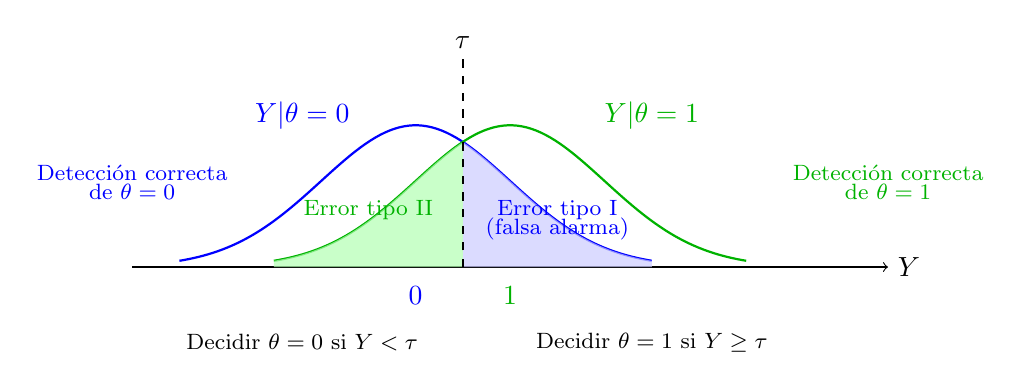
\begin{tikzpicture}[scale=1.2]
    % Eje horizontal
    \draw[->] (-3,0) -- (5,0) node[right] {$Y$};
    
    % Distribución Y|θ=0 (azul) - centrada en 0
    \draw[blue, thick] plot[domain=-2.5:2.5, samples=100] 
      (\x, {1.5*exp(-0.5*\x*\x)});
    \fill[blue!20, opacity=0.7] plot[domain=0.5:2.5, samples=50] 
      (\x, {1.5*exp(-0.5*\x*\x)}) -- (2.5,0) -- (0.5,0) -- cycle;
    
    % Distribución Y|θ=1 (verde) - centrada en 1
    \draw[green!70!black, thick] plot[domain=-1.5:3.5, samples=100] 
      (\x, {1.5*exp(-0.5*(\x-1)*(\x-1))});
    \fill[green!30, opacity=0.7] plot[domain=-1.5:0.5, samples=50] 
      (\x, {1.5*exp(-0.5*(\x-1)*(\x-1))}) -- (0.5,0) -- (-1.5,0) -- cycle;
    
    % Línea de decisión (umbral)
    \draw[dashed, thick] (0.5,0) -- (0.5,2.2) node[above] {$\tau$};
    
    % Etiquetas de las distribuciones
    \node[blue] at (-1.2,1.6) {$Y|\theta=0$};
    \node[green!70!black] at (2.5,1.6) {$Y|\theta=1$};
    
    % Valores de theta en el eje
    \node[blue] at (0,-0.3) {$0$};
    \node[green!70!black] at (1,-0.3) {$1$};
    
    % Etiquetas de probabilidades
    \node[blue] at (-3,1.0) {\footnotesize Detección correcta};
    \node[blue] at (-3,0.8) {\footnotesize de $\theta=0$};
    \node[blue] at (1.5,0.6) {\footnotesize Error tipo I};
    \node[blue] at (1.5,0.4) {\footnotesize (falsa alarma)};
    \node[green!70!black] at (-0.5,0.6) {\footnotesize Error tipo II};
    \node[green!70!black] at (5,1.0) {\footnotesize Detección correcta};
    \node[green!70!black] at (5,0.8) {\footnotesize de $\theta=1$};
    
    % Regiones de decisión
    \node at (-1.2,-0.8) {\footnotesize Decidir $\theta=0$ si $Y < \tau$};
    \node at (2.5,-0.8) {\footnotesize Decidir $\theta=1$ si $Y \geq \tau$};
    
  \end{tikzpicture}
  \caption{Distribuciones condicionales del problema de detección de señal: $Y|\theta=0 \sim \mathcal{N}(0, \sigma_0^2)$ y $Y|\theta=1 \sim \mathcal{N}(1, \sigma_0^2)$ con umbral de decisión $\tau$. Las regiones sombreadas ilustran los errores tipo I (falsa alarma) y tipo II.}
  \label{fig:canal_comunicacion}
  \end{figure}
\end{solution}
%----------------------------
\question Considere un canal binario simétrico con probabilidad de error $\varepsilon \in (0, 0.5)$, a través del cual se envía una palabra binaria $x = (s_1, \ldots, s_n) \in \{0,1\}^n$, de modo que se recibe la palabra $x = (s_1 \oplus \eta_1, \ldots, s_n \oplus \eta_n)$, donde $\eta_i \sim \text{Bernoulli}(\varepsilon)$ representa el ruido del canal, y $\oplus$ corresponde al operador XOR.

\begin{enumerate}
    \item Considere la distancia de Hamming, dada por
    \begin{equation}
    d(x; y) = \sum_{i=1}^{n} \mathbf{1}(x_i \neq y_i),
    \end{equation}
    donde $\mathbf{1}(\cdot)$ es la función indicatriz. Considere que la palabra enviada y recibida son variables aleatorias $S_1^n$ y $X_1^n$, respectivamente, y obtenga una expresión en términos de la distancia de Hamming para la verosimilitud del canal.
    
    \item Sea el conjunto $B_k(s) \subset \{0,1\}^n$ dado por
    \begin{equation}
    B_k(s) = \{x \in \{0,1\}^n : d(s; x) \leq k\},
    \end{equation}
    el cual representa las posibles palabras cuya distancia de Hamming a $s$ es a lo más $k$. Encuentre una expresión para
    \begin{equation}
    \eta_k \triangleq P_{X_1^n|S_1^n}(B_k(S_1^n)|S_1^n = (s_1, \ldots, s_n)).
    \end{equation}
    
    \item Considere las siguientes dos hipótesis: si $\theta = 0$ entonces $S_1^n = (0, \ldots, 0)$, y si $\theta = 1$ entonces $S_1^n = (1, \ldots, 1)$. Encuentre un test óptimo $\pi$ para detectar $\theta$ a partir de una medición $x$, cuyo tamaño sea $\alpha_\pi$.
\end{enumerate}
----------------------------
\begin{solution}
\subsection*{Resolución 3.1}

Notemos que buscamos obtener la verosimilitud, denotada por $f_{X_1^n|S_1^n}(x_1^n|s_1^n)$. Para esto, notemos que, si bien, en general, cada término de la palabra recibida no es necesariamente independiente del resto de símbolos, condicional a la palabra enviada sí lo son, ya que las diferencias símbolo a símbolo estarían explicadas únicamente por los ruidos $\eta_i^n$. Considerando esto, tenemos:

\begin{equation}
f_{X_1^n|S_1^n}(x_1^n|s_1^n) = \prod_{i=1}^n f_{X_i|S_i}(x_i|s_i).
\end{equation}

Por otra parte, notemos que el $i$-ésimo símbolo recibido depende, únicamente, del $i$-ésimo símbolo enviado, por lo que condicionar ante la palabra enviada total es equivalente a condicionar, únicamente, ante el $i$-ésimo símbolo, de modo que:

\begin{equation}
f_{X_1^n|S_1^n}(x_1^n|s_1^n) = \prod_{i=1}^n f_{X_i|S_i}(x_i|s_i).
\end{equation}

Luego, dado que $\forall i \in \{1, \ldots, n\}, \eta_i \sim \text{Bernoulli}(\varepsilon)$ tenemos:

\begin{equation}
f_{X_i|S_i}(x_i|s_i) = \varepsilon \mathbf{1}(x_i \neq s_i) + (1-\varepsilon) \mathbf{1}(x_i = s_i),
\end{equation}

por lo que:

\begin{equation}
f_{X_1^n|S_1^n}(x_1^n|s_1^n) = \prod_{i=1}^n [\varepsilon \mathbf{1}(x_i \neq s_i) + (1-\varepsilon) \mathbf{1}(x_i = s_i)].
\end{equation}

Utilizando intuición, intentemos obtener una expresión sucinta para la multiplicatoria. Notemos que, para cada bit $x_i$, tenemos dos opciones: $x_i = s_i$, en cuyo caso se aporta un término $1-\varepsilon$ a la multiplicatoria; o $x_i \neq s_i$, en cuyo caso se aporta un término $\varepsilon$. Realizando este análisis para todos los bits, $l$ sería el resultado de la multiplicatoria sería de la forma $\varepsilon^l (1-\varepsilon)^{n-l}$, con $D$ el número de bits distintos e $I$ el número de bits iguales entre $x_1^n$ y $s_1^n$. El número de bits distintos está dado por la distancia de Hamming $d(x_1^n; s_1^n)$ entre $x_1^n$ y $s_1^n$, mientras que el número de bits iguales está dado por $n - d(s_1^n; s_1^n)$. Luego, considerando todos los bits, tendríamos las iguales:

\begin{equation}
f_{X_1^n|S_1^n}(x_1^n|s_1^n) = \prod_{i=1}^n [\varepsilon \mathbf{1}(x_i \neq s_i) + (1-\varepsilon) \mathbf{1}(x_i = s_i)] = \varepsilon^{d(x_1^n;s_1^n)} (1-\varepsilon)^{n-d(x_1^n;s_1^n)}.
\end{equation}

Sin embargo, notemos que no tenemos una demostración rigurosa de que la expresión obtenida es realmente válida. Para poder validar que realmente se cumple lo planteado, hagamos una demostración por inducción.

Para el caso base $n = 1$, es fácil ver que si los mensajes son iguales tenemos $f_{X_1|S_1}(x_1^1|s_1^1) = 1-\varepsilon$ y, si son distintos, tenemos $f_{X_1|S_1}(x_1^1|s_1^1) = \varepsilon$. Luego, supongamos que la expresión dada se cumple para un $n$ dado.

Para $n+1$ tendremos:

\begin{equation}
f_{X_1^{n+1}|S_1^{n+1}}(x_1^{n+1}|s_1^{n+1}) = \prod_{i=1}^{n+1} [\varepsilon \mathbf{1}(x_i \neq s_i) + (1-\varepsilon) \mathbf{1}(x_i = s_i)].
\end{equation}

Si sacamos el término $(n+1)$-ésimo de la multiplicatoria, podemos expresar la probabilidad como:

\begin{equation}
f_{X_1^{n+1}|S_1^{n+1}}(x_1^{n+1}|s_1^{n+1}) = [\varepsilon \mathbf{1}(x_{n+1} \neq s_{n+1}) + (1-\varepsilon) \mathbf{1}(x_{n+1} = s_{n+1})] f_{X_1^n|S_1^n}(x_1^n|s_1^n).
\end{equation}

Por la hipótesis inductiva sabemos que se tiene:

\begin{equation}
f_{X_1^n|S_1^n}(x_1^n|s_1^n) = \prod_{i=1}^n [\varepsilon \mathbf{1}(x_i \neq s_i) + (1-\varepsilon) \mathbf{1}(x_i = s_i)] = \varepsilon^{d(x_1^n;s_1^n)} (1-\varepsilon)^{n-d(x_1^n;s_1^n)},
\end{equation}

donde $d(x_1^n; s_1^n)$ correspondería a la distancia de Hamming entre ambas palabras hasta el $n$-ésimo bit, por lo que podemos escribir la ecuación 10 como:

\begin{align}
f_{X_1^{n+1}|S_1^{n+1}}(x_1^{n+1}|s_1^{n+1}) &= [\varepsilon \mathbf{1}(x_{n+1} \neq s_{n+1}) + (1-\varepsilon) \mathbf{1}(x_{n+1} = s_{n+1})] \varepsilon^{d(x_1^n;s_1^n)} (1-\varepsilon)^{n-d(x_1^n;s_1^n)} \\
\end{align}

Para proceder, hagamos un análisis por casos en términos de si $x_{n+1}$ y $s_{n+1}$ son iguales o no. Antes de esto, comencemos notando que podemos escribir la distancia de Hamming hasta el término $n+1$ como:

\begin{align}
d(x_1^{n+1}, s_1^{n+1}) = \sum_{i=1}^{n+1} \mathbf{1}(x_i \neq s_i) &= \mathbf{1}(x_{n+1} \neq s_{n+1}) + \sum_{i=1}^n \mathbf{1}(x_i \neq s_i) \\
&\Rightarrow d(x_1^{n+1}, s_1^{n+1}) = \mathbf{1}(x_{n+1} \neq s_{n+1}) + d(x_1^n; s_1^n).
\end{align}

\textbf{Caso 1:} Para el caso 1, supongamos que $x_{n+1} \neq s_{n+1}$. En este caso, por la ecuación 14 podemos ver que $d(x_1^{n+1}, s_1^{n+1}) = d(x_1^n; s_1^n) + 1$. Considerando esto desde de la ecuación 12, tenemos:

\begin{align}
f_{X_1^{n+1}|S_1^{n+1}}(x_1^{n+1}|s_1^{n+1}) &= [\varepsilon \mathbf{1}(x_{n+1} \neq s_{n+1}) + (1-\varepsilon) \mathbf{1}(x_{n+1} = s_{n+1})] \varepsilon^{d(x_1^n;s_1^n)} (1-\varepsilon)^{n-d(x_1^n;s_1^n)} \\
&= \varepsilon \varepsilon^{d(x_1^n;s_1^n)} (1-\varepsilon)^{n-d(x_1^n;s_1^n)} \\
&= \varepsilon^{d(x_1^n;s_1^n)+1} (1-\varepsilon)^{n-d(x_1^n;s_1^n)}
\end{align}

Notemos que, de acuerdo a lo encontrado, se cumple $d(x_1^n; s_1^n) = d(x_1^{n+1}, s_1^{n+1}) - 1$, por lo que tenemos:

\begin{align}
f_{X_1^{n+1}|S_1^{n+1}}(x_1^{n+1}|s_1^{n+1}) &= \varepsilon^{d(x_1^{n+1}, s_1^{n+1})} (1-\varepsilon)^{n-d(x_1^{n+1}, s_1^{n+1})+1} \\
&= \varepsilon^{d(x_1^{n+1}, s_1^{n+1})} (1-\varepsilon)^{n+1-d(x_1^{n+1}, s_1^{n+1})},
\end{align}

lo cual corresponde a lo que buscábamos demostrar, demostrando que es válido para el caso en que $x_{n+1} \neq s_{n+1}$.

\textbf{Caso 2:} Para el caso 2, supongamos que $x_{n+1} = s_{n+1}$. Con esto, podemos ver que las distancias de Hamming cumplen que $d(x_1^{n+1}, s_1^{n+1}) = d(x_1^n; s_1^n)$. Evaluando en la ecuación 12, tenemos:

\begin{align}
f_{X_1^{n+1}|S_1^{n+1}}(x_1^{n+1}|s_1^{n+1}) &= [\varepsilon \mathbf{1}(x_{n+1} \neq s_{n+1}) + (1-\varepsilon) \mathbf{1}(x_{n+1} = s_{n+1})] \varepsilon^{d(x_1^n;s_1^n)} (1-\varepsilon)^{n-d(x_1^n;s_1^n)} \\
&= (1-\varepsilon) \varepsilon^{d(x_1^n;s_1^n)} (1-\varepsilon)^{n-d(x_1^n;s_1^n)} \\
&= \varepsilon^{d(x_1^n;s_1^n)} (1-\varepsilon)^{n+1-d(x_1^n;s_1^n)} \\
&= \varepsilon^{d(x_1^{n+1}, s_1^{n+1})} (1-\varepsilon)^{n+1-d(x_1^{n+1}, s_1^{n+1})},
\end{align}

lo cual, nuevamente, cumple con lo que buscamos demostrar. Esto permite verificar que la expresión encontrada para la probabilidad es válida, por lo que tenemos:

\begin{equation}
f_{X_1^n|S_1^n}(x_1^n|s_1^n) = \varepsilon^{d(x_1^n;s_1^n)} (1-\varepsilon)^{n-d(x_1^n;s_1^n)}.
\end{equation}

\subsection*{Resolución 3.2}

\textbf{Probabilidad de distancia de Hamming}

Durante el desarrollo de la clase me di cuenta que usé la misma variable tanto para el ruido como para la probabilidad. Por lo tanto, la variable de la probabilidad la reemplacé por $\eta_k$, de modo que:

\begin{equation}
\eta_k(s_1^n) \triangleq P_{X_1^n|S_1^n}(X_1^n \in B_k(S_1^n)|S_1^n = s_1^n).
\end{equation}

Para obtener la expresión solicitada, comencemos notando que podemos separar el conjunto $B_k(s_1^n)$ como:

\begin{equation}
B_k(s_1^n) = \{x_1^n \in \{0,1\}^n | d(x_1^n; s_1^n) \leq k\} = \bigcup_{i=0}^k \{x_1^n \in \{0,1\}^n | d(x_1^n; s_1^n) = i\},
\end{equation}

donde $\forall i, j, C_i(s_1^n) \cap C_j(s_1^n) = \emptyset$ por lo que $C_i(s_1^n)$ y $C_j(s_1^n)$ son disjuntos. La forma en que podemos interpretar cada $C_i(s_1^n)$ es el conjunto de posibles palabras $x^n$ que están a una distancia de Hamming $i$ de la palabra $s_1^n$, y, por ende, $B_k(s_1^n)$ correspondería al conjunto de palabras con distancia de Hamming menor o igual a $k$.

Luego, dado que los conjuntos son disjuntos, podemos escribir $\eta_k(s_1^n)$ como:

\begin{equation}
\eta_k(s_1^n) = P_{X_1^n|S_1^n}(X_1^n \in B_k(S_1^n)|S_1^n = s_1^n) = \sum_{i=0}^k P_{X_1^n|S_1^n}(X_1^n \in C_i(S_1^n)|S_1^n = s_1^n).
\end{equation}

Por la forma en que está definido cada conjunto $C_i$, podemos escribir cada una de las probabilidades $P_{X_1^n|S_1^n}(X_1^n \in C_i(S_1^n)|S_1^n = s_1^n)$ como:

\begin{equation}
P_{X_1^n|S_1^n}(X_1^n \in C_i(S_1^n)|S_1^n = s_1^n) = P_{X_1^n|S_1^n}(d(X_1^n; S_1^n) = i|S_1^n = s_1^n)
\end{equation}

donde, reemplazando la definición de la distancia de Hamming, tenemos:

\begin{equation}
P_{X_1^n|S_1^n}(X_1^n \in C_i(S_1^n)|S_1^n = s_1^n) = P_{X_1^n|S_1^n}\left(\sum_{j=1}^n \mathbf{1}(X_j \neq S_j) = i|S_1^n = s_1^n\right).
\end{equation}

Luego, notemos que, para cada término de la sumatoria, al condicionar ante $S_1^n = s_1^n$ podemos ver que se tiene $\mathbf{1}(X_j \neq S_j) = \mathbf{1}(s_j \neq \eta_j \neq s_j) = \mathbf{1}(\eta_j = 1)$, donde, dado que $\eta_j \in \{0,1\}$, tenemos $\mathbf{1}(\eta_j = 1) = \eta_j$, de modo que podemos escribir la probabilidad anterior en términos de cada término del ruido como:

\begin{equation}
P_{X_1^n|S_1^n}(X_1^n \in C_i(S_1^n)|S_1^n = s_1^n) = P_{\eta}\left(\sum_{j=1}^n \eta_j = i\right).
\end{equation}

Luego, dado que $\forall j \in \{1, \ldots, n\}, \eta_j \sim \text{Bernoulli}(\varepsilon)$, y dado que los ruidos son i.i.d., por propiedades de la distribución Bernoulli sabemos que $\sum_{j=1}^n \eta_j \sim \text{Binomial}(n, \varepsilon)$, por lo que:

\begin{equation}
P_{\eta}\left(\sum_{j=1}^n \eta_j = i\right) = \binom{n}{i} \varepsilon^i (1-\varepsilon)^{n-i}.
\end{equation}

Así, tenemos:

\begin{equation}
P_{X_1^n|S_1^n}(X_1^n \in C_i(S_1^n)|S_1^n = s_1^n) = \binom{n}{i} \varepsilon^i (1-\varepsilon)^{n-i},
\end{equation}

de modo que:

\begin{equation}
\eta_k(s_1^n) = \sum_{i=0}^k \binom{n}{i} \varepsilon^i (1-\varepsilon)^{n-i}.
\end{equation}

\subsection*{Resolución 3.3}

Para plantear la regla óptima, notemos que, por lema de Neyman-Pearson, sabemos que cualquier regla óptima sería de la forma:

\begin{equation}
\pi^*(\rho, X_1^n) = \begin{cases}
1 & \text{si } L(X_1^n|\theta = 1) > \nu L(X_1^n|\theta = 0) \\
\rho & \text{si } L(X_1^n|\theta = 1) = \nu L(X_1^n|\theta = 0) \\
0 & \text{si } L(X_1^n|\theta = 1) < \nu L(X_1^n|\theta = 0)
\end{cases}
\end{equation}

donde $L(X_1^n|\theta)$ corresponde a la verosimilitud que encontramos anteriormente, donde, tomando en consideración que si $\theta = 0$ entonces $S_1^n = (0, \ldots, 0) \triangleq s_0$ y si $\theta = 1$ entonces $S_1^n = (1, \ldots, 1) \triangleq s_1$, podemos ver que:

\begin{align}
L(X_1^n|\theta = 1) &= \varepsilon^{d(X_1^n;s_1)} (1-\varepsilon)^{n-d(X_1^n;s_1)} \\
L(X_1^n|\theta = 0) &= \varepsilon^{d(X_1^n;s_0)} (1-\varepsilon)^{n-d(X_1^n;s_0)}.
\end{align}

Si, además, denotamos $\ell(X_1^n)$ a la razón de verosimilitud, dada por:

\begin{equation}
\ell(X_1^n) \triangleq \frac{L(X_1^n|\theta = 1)}{L(X_1^n|\theta = 0)},
\end{equation}

podemos replantear la regla óptima como:

\begin{equation}
\pi^*(\rho, X_1^n) = \begin{cases}
1 & \text{si } \ell(X_1^n) > \nu \\
\rho & \text{si } \ell(X_1^n) = \nu \\
0 & \text{si } \ell(X_1^n) < \nu
\end{cases}
\end{equation}

Para desarrollar la razón de verosimilitud, comencemos analizando las distancias de Hamming a cada palabra de la codificación. Notemos que:

\begin{align}
d(X_1^n; s_0) &= \sum_{i=1}^n \mathbf{1}(X_i \neq 0) \\
d(X_1^n; s_1) &= \sum_{i=1}^n \mathbf{1}(X_i \neq 1),
\end{align}

por lo que:

\begin{equation}
d(X_1^n; s_0) + d(X_1^n; s_1) = \sum_{i=1}^n [\mathbf{1}(X_i \neq 0) + \mathbf{1}(X_i \neq 1)] = n,
\end{equation}

de modo que se tiene $d(X_1^n; s_0) = n - d(X_1^n; s_1)$ y $d(X_1^n; s_0) = n - d(X_1^n; s_1)$.

Luego, desarrollemos la razón de verosimilitud, tratando de dejar todo en función de la distancia a la palabra $s_0$. Al hacerlo, tenemos:

\begin{align}
\ell(X_1^n) &= \frac{\varepsilon^{d(X_1^n;s_1)} (1-\varepsilon)^{n-d(X_1^n;s_1)}}{\varepsilon^{d(X_1^n;s_0)} (1-\varepsilon)^{n-d(X_1^n;s_0)}} \\
&= \frac{\varepsilon^{n-d(X_1^n;s_0)} (1-\varepsilon)^{d(X_1^n;s_0)}}{\varepsilon^{d(X_1^n;s_0)} (1-\varepsilon)^{n-d(X_1^n;s_0)}} \\
&= \left(\frac{1-\varepsilon}{\varepsilon}\right)^{2d(X_1^n;s_0)-n}.
\end{align}

Así, si nos enfocamos en el caso donde $\pi^*(\rho, X_1^n) = 1$, teniendo en consideración que los otros dos casos serían análogos, notemos que $\pi^*(\rho, X_1^n) = 1$ ssi $\ell(X_1^n) > \nu$:

\begin{align}
&\Leftrightarrow \left(\frac{1-\varepsilon}{\varepsilon}\right)^{2d(X_1^n;s_0)-n} > \nu \\
&\Leftrightarrow (2d(X_1^n; s_0) - n) \log\left(\frac{1-\varepsilon}{\varepsilon}\right) > \log(\nu).
\end{align}

Si despejamos la distancia a la palabra $s_0$, tenemos:

\begin{equation}
d(X_1^n; s_0) > \frac{n}{2} + \frac{\log(\nu)}{2\log\left(\frac{1-\varepsilon}{\varepsilon}\right)},
\end{equation}

de modo que la regla óptima es de la forma:

\begin{equation}
\pi^*(\rho, X_1^n) = \begin{cases}
1 & \text{si } d(X_1^n; s_0) > \frac{n}{2} + \frac{\log(\nu)}{2\log\left(\frac{1-\varepsilon}{\varepsilon}\right)} \\
\rho & \text{si } d(X_1^n; s_0) = \frac{n}{2} + \frac{\log(\nu)}{2\log\left(\frac{1-\varepsilon}{\varepsilon}\right)} \\
0 & \text{si } d(X_1^n; s_0) < \frac{n}{2} + \frac{\log(\nu)}{2\log\left(\frac{1-\varepsilon}{\varepsilon}\right)}
\end{cases}
\end{equation}

Por último, queremos que el tamaño del test sea igual a un cierto valor $\alpha$ arbitrario, para lo cual, si consideramos que $\rho \sim \text{Bernoulli}(p)$, debemos determinar los valores de $p$ y $\nu$ tales que $\alpha_{\pi^*} = \alpha$. Comencemos notando que el tamaño del test corresponde a:

\begin{equation}
\alpha_{\pi^*} = E_{\theta,X_1^n}[\pi^*(\rho, X_1^n)|\theta = 0],
\end{equation}

lo cual se puede reescribir como:

\begin{equation}
\alpha_{\pi^*} = P_{X_1^n}(\ell(X_1^n) > \nu|\theta = 0) + p P_{X_1^n}(\ell(X_1^n) = \nu|\theta = 0).
\end{equation}

Expresemos cada término por separado. Comenzando por el término de la izquierda, tenemos:

\begin{equation}
P_{X_1^n}(\ell(X_1^n) > \nu|\theta = 0) = P_{X_1^n}(d(X_1^n; s_0) > \tau(\nu)|\theta = 0) = 1 - P_{X_1^n}(d(X_1^n; s_0) \leq \tau(\nu)|\theta = 0),
\end{equation}

donde:

\begin{equation}
\tau(\nu) \triangleq \frac{n}{2} + \frac{\log(\nu)}{2\log\left(\frac{1-\varepsilon}{\varepsilon}\right)}
\end{equation}

denota el umbral utilizado. Podemos ver que la probabilidad corresponde a $\gamma_{\tau(\nu)}(s_0)$ calculado anteriormente, donde tomamos el piso de $\tau(\nu)$ dado que, en general, este puede ser cualquier número real. De este modo, tenemos:

\begin{equation}
P_{X_1^n}(\ell(X_1^n) > \nu|\theta = 0) = 1 - \gamma_{\lfloor\tau(\nu)\rfloor}(s_0).
\end{equation}

Por otra parte, para el término de la derecha tenemos:

\begin{equation}
P_{X_1^n}(\ell(X_1^n) = \nu|\theta = 0) = P_{X_1^n}(d(X_1^n; s_0) = \tau(\nu)|\theta = 0).
\end{equation}

Notemos que, dependiendo de si $\tau(\nu)$ es un número natural o no, esta probabilidad puede o no tomar un valor. En particular, si $\tau(\nu)$ no es un número natural, entonces la probabilidad es 0, mientras que si es un número natural, la probabilidad correspondería a:

\begin{equation}
P_{X_1^n}(\ell(X_1^n) = \nu|\theta = 0) = \left(\frac{n}{\tau(\nu)}\right) \varepsilon^{\tau(\nu)} (1-\varepsilon)^{n-\tau(\nu)} \mathbf{1}_{\mathbb{N}}(\tau(\nu)).
\end{equation}

Podemos juntar estos dos casos utilizando una indicatriz, de modo que:

\begin{equation}
P_{X_1^n}(\ell(X_1^n) = \nu|\theta = 0) = \left(\frac{n}{\tau(\nu)}\right) \varepsilon^{\tau(\nu)} (1-\varepsilon)^{n-\tau(\nu)} \mathbf{1}_{\mathbb{N}}(\tau(\nu)).
\end{equation}

Así, tenemos que el tamaño de la regla óptima está dado por:

\begin{equation}
\alpha_{\pi^*} = 1 - \gamma_{\lfloor\tau(\nu)\rfloor}(s_0) + p \left(\frac{n}{\tau(\nu)}\right) \varepsilon^{\tau(\nu)} (1-\varepsilon)^{n-\tau(\nu)} \mathbf{1}_{\mathbb{N}}(\tau(\nu)),
\end{equation}

por lo que el objetivo sería encontrar $p$ y $\nu$ tales que:

\begin{equation}
1 - \gamma_{\lfloor\tau(\nu)\rfloor}(s_0) + p \left(\frac{n}{\tau(\nu)}\right) \varepsilon^{\tau(\nu)} (1-\varepsilon)^{n-\tau(\nu)} \mathbf{1}_{\mathbb{N}}(\tau(\nu)) = \alpha_{\pi^*}.
\end{equation}

Sin embargo, podemos ver que las relaciones que se tienen no son invertibles, por lo que no sería posible encontrar los parámetros de forma analítica y, para poder hacerlo, sería necesario recurrir a técnicas numéricas, ya sea resolviendo la ecuación 58 numéricamente o construyendo una curva ROC y, a partir de esta, determinando el valor de los parámetros.
\end{solution}
%----------------------------
\question Una máquina de acuñación defectuosa produce monedas cuya probabilidad de obtener cara es una variable aleatoria $P$ con PDF
\begin{equation}
f_P(p) = \begin{cases}
1 + \sin(2\pi p), & \text{si } p \in [0,1], \\
0, & \text{en otro caso}.
\end{cases}
\end{equation}

En esencia, una moneda específica producida por esta máquina tendrá una probabilidad fija $P = p$ de dar cara, pero usted no conoce inicialmente cuál es esa probabilidad. Una moneda producida por esta máquina es seleccionada y lanzada repetidamente, con lanzamientos sucesivos asumidos independientes.

\begin{enumerate}
    \item Encuentre la probabilidad de que el primer lanzamiento de la moneda resulte en cara.
    
    \item Dado que el primer lanzamiento de la moneda resultó en cara, encuentre la PDF condicional de $P$.
    
    \item Dado que el primer lanzamiento de la moneda resultó en cara, encuentre la probabilidad condicional de obtener cara en el segundo lanzamiento.
\end{enumerate}
%----------------------------
\begin{solution}
  \subsection*{Resolución 3.1}

Primero, es crucial entender qué representa cada elemento del problema:

\begin{itemize}
\item \textbf{La variable $P$:} No es un número fijo, sino una \emph{variable aleatoria} que representa la probabilidad de obtener cara de una moneda específica producida por la máquina defectuosa. Cada moneda que produce la máquina tiene su propia probabilidad $P$ de dar cara, pero esta probabilidad varía de moneda a moneda.

\item \textbf{La distribución $f_P(p) = 1 + \sin(2\pi p)$:} Esta función nos dice qué tan probable es que una moneda producida por la máquina tenga probabilidad $p$ de dar cara. Es una distribución que:
\begin{itemize}
\item Oscila entre $1 - 1 = 0$ y $1 + 1 = 2$
\item Tiene máximos en $p = 0.25$ y $p = 0.75$ (donde $\sin(2\pi p) = 1$)
\item Tiene mínimos en $p = 0$ y $p = 0.5$ y $p = 1$ (donde $\sin(2\pi p) = 0$ o $-1$)
\item Esto significa que la máquina tiende a producir monedas sesgadas hacia $p = 0.25$ o $p = 0.75$, pero raramente produce monedas justas ($p = 0.5$)
\end{itemize}

\item \textbf{El proceso:} Tomamos una moneda al azar de las producidas por esta máquina defectuosa. No sabemos cuál es su probabilidad específica $P$, solo sabemos que sigue la distribución dada.
\end{itemize}

El problema fundamental aquí es que no conocemos el valor exacto de la probabilidad $P$ de la moneda específica que tenemos. Esto significa que debemos considerar todos los posibles valores que $P$ puede tomar, ponderando cada uno por su probabilidad de ocurrencia según la distribución $f_P(p)$ que nos proporciona el enunciado.

Para calcular la probabilidad $\mathbb{P}(A)$, usamos la versión continua del teorema de probabilidad total:

\begin{equation}
\mathbb{P}(A) = \int_0^1 \mathbb{P}(A | P = p)f_P(p) \, dp = \int_0^1 p(1 + \sin(2\pi p)) \, dp,
\end{equation}

donde $\mathbb{P}(A | P = p) = p$ porque si la moneda tiene probabilidad fija $p$ de dar cara, entonces la probabilidad de obtener cara es exactamente $p$. Separamos la integral en dos partes:
\begin{equation}
\mathbb{P}(A) = \int_0^1 p \, dp + \int_0^1 p \sin(2\pi p) \, dp
\end{equation}

La primera integral es directa:
\begin{equation}
\int_0^1 p \, dp = \left[\frac{p^2}{2}\right]_0^1 = \frac{1^2}{2} - \frac{0^2}{2} = \frac{1}{2}
\end{equation}


Para la segunda integral, $\int_0^1 p \sin(2\pi p) \, dp$, usamos integración por partes con:
\begin{align}
u &= p \quad \Rightarrow \quad du = dp \\
dv &= \sin(2\pi p) \, dp \quad \Rightarrow \quad v = -\frac{1}{2\pi}\cos(2\pi p)
\end{align}

Aplicando la fórmula de integración por partes $\int u \, dv = uv - \int v \, du$:
\begin{align}
\int_0^1 p \sin(2\pi p) \, dp &= \left[p \cdot \left(-\frac{1}{2\pi}\cos(2\pi p)\right)\right]_0^1 - \int_0^1 \left(-\frac{1}{2\pi}\cos(2\pi p)\right) dp \\
&= \left[-\frac{p}{2\pi}\cos(2\pi p)\right]_0^1 + \frac{1}{2\pi}\int_0^1 \cos(2\pi p) \, dp
\end{align}

Evaluamos cada término por separado:
\begin{itemize}
  \item \textbf{Primer término:}
\begin{align}
\left[-\frac{p}{2\pi}\cos(2\pi p)\right]_0^1 &= -\frac{1}{2\pi}\cos(2\pi \cdot 1) - \left(-\frac{0}{2\pi}\cos(2\pi \cdot 0)\right) \\
&= -\frac{1}{2\pi}\cos(2\pi) - 0 \\
&= -\frac{1}{2\pi} \cdot 1 = -\frac{1}{2\pi}
\end{align}

donde usamos que $\cos(2\pi) = 1$.

\item \textbf{Segundo término:}
\begin{align}
\frac{1}{2\pi}\int_0^1 \cos(2\pi p) \, dp &= \frac{1}{2\pi} \left[\frac{1}{2\pi}\sin(2\pi p)\right]_0^1 \\
&= \frac{1}{(2\pi)^2}[\sin(2\pi \cdot 1) - \sin(2\pi \cdot 0)] \\
&= \frac{1}{4\pi^2}[0 - 0] = 0
\end{align}

donde usamos que $\sin(2\pi) = \sin(0) = 0$.
\end{itemize}
Por tanto:
\begin{equation}
\int_0^1 p \sin(2\pi p) \, dp = -\frac{1}{2\pi} + 0 = -\frac{1}{2\pi}
\end{equation}

Combinando ambas integrales:
\begin{align}
\mathbb{P}(A) &= \int_0^1 p \, dp + \int_0^1 p \sin(2\pi p) \, dp \\
&= \frac{1}{2} + \left(-\frac{1}{2\pi}\right) \\
&= \frac{1}{2} - \frac{1}{2\pi} \\
&= \frac{\pi - 1}{2\pi} \approx 0.341
\end{align}


El resultado $\mathbb{P}(A) = \frac{\pi - 1}{2\pi} \approx 0.341 < 0.5$ tiene sentido intuitivo:

\begin{itemize}
\item Si todas las monedas fueran justas ($P = 0.5$ siempre), tendríamos $\mathbb{P}(A) = 0.5$
\item Si la distribución fuera uniforme ($f_P(p) = 1$), también tendríamos $\mathbb{P}(A) = 0.5$
\item Pero nuestra distribución $f_P(p) = 1 + \sin(2\pi p)$ favorece valores como $p = 0.25$ y $p = 0.75$
\item El término $-\frac{1}{2\pi}$ proviene del componente sinusoidal y refleja el sesgo de la distribución
\item Como la distribución le da más peso relativo a monedas con probabilidades menores (especialmente $p = 0.25$), el resultado global es menor que $0.5$
\end{itemize}\subsection*{Resolución 3.2}

Imagina que inicialmente no sabemos nada específico sobre nuestra moneda, solo que viene de la máquina defectuosa. Pero cuando lanzamos la moneda y sale cara, esta observación nos da información valiosa

\begin{itemize}
\item \textbf{Antes del lanzamiento:} Cualquier moneda podría tener probabilidades desde $p = 0$ hasta $p = 1$, pero algunas son más probables según $f_P(p) = 1 + \sin(2\pi p)$
\item \textbf{Después de observar cara:} Las monedas con $p$ muy pequeño (digamos $p = 0.1$) se vuelven menos creíbles, mientras que las monedas con $p$ más grande (digamos $p = 0.8$) se vuelven más creíbles
\item Esto porque si una moneda tiene $p = 0.1$, es muy raro que dé cara, pero si tiene $p = 0.8$, es bastante común que dé cara
\end{itemize}

La situación cambia fundamentalmente cuando observamos que el primer lanzamiento dio cara. Esta nueva información nos permite actualizar nuestro conocimiento sobre la distribución de $P$ usando inferencia bayesiana. La observación nos proporciona evidencia que modifica nuestra creencia inicial sobre qué valores de $P$ son más probables.

Recordemos que la regla de Bayes viene dada por:
\begin{equation}
\mathbb{P}(H | E) = \frac{\mathbb{P}(E | H) \mathbb{P}(H)}{\mathbb{P}(E)}
\end{equation}
donde $H$ es una hipótesis (en este caso, un valor específico de $P$) y $E$ es la evidencia observada (el evento de obtener cara). Usando la regla de Bayes para encontrar la distribución posterior de $P$ dado que observamos cara:

\begin{equation}
f_{P|A}(p) = \frac{\mathbb{P}(A | P = p)f_P(p)}{\mathbb{P}(A)}
\end{equation}

Donde:
\begin{itemize}
\item $\mathbb{P}(A | P = p) = p$ (si la moneda tiene probabilidad $p$, entonces la probabilidad de cara es $p$)
\item $f_P(p) = 1 + \sin(2\pi p)$ (distribución original de la máquina)
\item $\mathbb{P}(A) = \frac{\pi - 1}{2\pi}$ (calculado en la parte anterior)
\end{itemize}

Sustituyendo:
\begin{equation}
f_{P|A}(p) = \frac{p \cdot (1 + \sin(2\pi p))}{\frac{\pi - 1}{2\pi}} = \frac{2\pi p(1 + \sin(2\pi p))}{\pi - 1}
\end{equation}

Por tanto:
\begin{equation}
f_{P|A}(p) = \begin{cases}
\frac{2\pi p(1 + \sin(2\pi p))}{\pi - 1}, & \text{si } 0 \leq p \leq 1, \\
0, & \text{en otro caso}.
\end{cases}
\end{equation}

Comparando $f_{P|A}(p)$ con la distribución original $f_P(p)$:
\begin{itemize}
\item La nueva distribución tiene un factor adicional de $p$ en el numerador
\item Esto significa que valores más grandes de $p$ reciben mayor peso relativo
\item Por ejemplo: si $p = 0.1$, el factor $p = 0.1$ reduce la probabilidad; si $p = 0.8$, el factor $p = 0.8$ la aumenta considerablemente
\item Después de observar una cara, es más probable que nuestra moneda tenga una probabilidad alta de dar cara
\end{itemize}

\subsection*{Resolución 3.3}

Ahora queremos predecir el segundo lanzamiento, pero con una ventaja: \emph{ya sabemos que el primer lanzamiento dio cara}. Esta información cambia todo nuestro análisis.


\begin{itemize}
\item \textbf{Situación inicial:} Tenemos una moneda de la máquina defectuosa y el primer lanzamiento dio cara
\item \textbf{Lo que sabemos ahora:} Gracias al primer lanzamiento, tenemos una mejor idea de qué tipo de moneda es (distribución actualizada $f_{P|A}(p)$)
\item \textbf{Lo que queremos:} La probabilidad de que el segundo lanzamiento también sea cara
\item \textbf{Clave importante:} Los lanzamientos son independientes \emph{dado el valor de $P$}, pero como no conocemos $P$ exactamente, hay dependencia estadística entre los lanzamientos
\end{itemize}

Para predecir el resultado del segundo lanzamiento, debemos utilizar toda la información disponible. Esto significa que ya no usamos la distribución original $f_P(p)$, sino la distribución actualizada $f_{P|A}(p)$ que incorpora la información del primer lanzamiento. 

Es importante recordar que los lanzamientos son independientes condicionalmente a $P$, lo que significa que una vez que conocemos (o tenemos una distribución sobre) el valor de $P$, los resultados de diferentes lanzamientos no se influyen mutuamente. Tenemos:
\begin{align}
\mathbb{P}(B | A) &= \int_0^1 \mathbb{P}(B | P = p, A)f_{P|A}(p) \, dp \\
&= \int_0^1 \mathbb{P}(B | P = p)f_{P|A}(p) \, dp \\
&= \frac{2\pi}{\pi - 1} \int_0^1 p^2(1 + \sin(2\pi p)) \, dp.
\end{align}

\textbf{Explicación de cada paso:}
\begin{itemize}
\item \textbf{Primera línea:} Usamos el teorema de probabilidad total, pero ahora con la distribución actualizada $f_{P|A}(p)$
\item \textbf{Segunda línea:} Aplicamos independencia condicional: $\mathbb{P}(B | P = p, A) = \mathbb{P}(B | P = p) = p$
\item \textbf{¿Por qué independencia condicional?} Si sabemos que $P = p$, entonces el resultado del primer lanzamiento no afecta directamente al segundo; ambos solo dependen de $p$
\item \textbf{Tercera línea:} Sustituimos $f_{P|A}(p) = \frac{2\pi p(1 + \sin(2\pi p))}{\pi - 1}$
\end{itemize}


Observa que ahora tenemos $p^2$ en la integral (comparado con solo $p$ en la parte (a)). Este $p^2$ proviene de:
\begin{itemize}
\item Un factor $p$ de $\mathbb{P}(B | P = p) = p$ (probabilidad del segundo lanzamiento)
\item Un factor $p$ de $f_{P|A}(p)$ (la actualización bayesiana que favorece valores grandes de $p$)
\end{itemize}

Necesitamos calcular:
\begin{equation}
\int_0^1 p^2(1 + \sin(2\pi p)) \, dp
\end{equation}

Separamos la integral en dos partes:
\begin{equation}
\int_0^1 p^2(1 + \sin(2\pi p)) \, dp = \int_0^1 p^2 \, dp + \int_0^1 p^2 \sin(2\pi p) \, dp
\end{equation}

\textbf{Primera integral:}
\begin{equation}
\int_0^1 p^2 \, dp = \left[\frac{p^3}{3}\right]_0^1 = \frac{1^3}{3} - \frac{0^3}{3} = \frac{1}{3}
\end{equation}

\textbf{Segunda integral:}
Para $\int_0^1 p^2 \sin(2\pi p) \, dp$, usamos integración por partes dos veces.

\begin{align}
u &= p^2 \quad \Rightarrow \quad du = 2p \, dp \\
dv &= \sin(2\pi p) \, dp \quad \Rightarrow \quad v = -\frac{1}{2\pi}\cos(2\pi p)
\end{align}

\begin{align}
\int_0^1 p^2 \sin(2\pi p) \, dp &= \left[p^2 \cdot \left(-\frac{1}{2\pi}\cos(2\pi p)\right)\right]_0^1 - \int_0^1 \left(-\frac{1}{2\pi}\cos(2\pi p)\right) \cdot 2p \, dp \\
&= \left[-\frac{p^2}{2\pi}\cos(2\pi p)\right]_0^1 + \frac{1}{\pi}\int_0^1 p \cos(2\pi p) \, dp
\end{align}

Evaluando el primer término:
\begin{align}
\left[-\frac{p^2}{2\pi}\cos(2\pi p)\right]_0^1 &= -\frac{1^2}{2\pi}\cos(2\pi) - \left(-\frac{0^2}{2\pi}\cos(0)\right) \\
&= -\frac{1}{2\pi} \cdot 1 - 0 = -\frac{1}{2\pi}
\end{align}

\textbf{Segunda integración por partes} para $\int_0^1 p \cos(2\pi p) \, dp$:
\begin{align}
u &= p \quad \Rightarrow \quad du = dp \\
dv &= \cos(2\pi p) \, dp \quad \Rightarrow \quad v = \frac{1}{2\pi}\sin(2\pi p)
\end{align}

\begin{align}
\int_0^1 p \cos(2\pi p) \, dp &= \left[p \cdot \frac{1}{2\pi}\sin(2\pi p)\right]_0^1 - \int_0^1 \frac{1}{2\pi}\sin(2\pi p) \, dp \\
&= \left[\frac{p}{2\pi}\sin(2\pi p)\right]_0^1 + \frac{1}{2\pi}\int_0^1 \sin(2\pi p) \, dp \\
&= 0 + \frac{1}{2\pi} \left[-\frac{1}{2\pi}\cos(2\pi p)\right]_0^1 \\
&= -\frac{1}{4\pi^2}[\cos(2\pi) - \cos(0)] = -\frac{1}{4\pi^2}[1 - 1] = 0
\end{align}

Por tanto:
\begin{equation}
\int_0^1 p^2 \sin(2\pi p) \, dp = -\frac{1}{2\pi} + \frac{1}{\pi} \cdot 0 = -\frac{1}{2\pi}
\end{equation}

Combinando ambas integrales:
\begin{align}
\int_0^1 p^2(1 + \sin(2\pi p)) \, dp &= \int_0^1 p^2 \, dp + \int_0^1 p^2 \sin(2\pi p) \, dp \\
&= \frac{1}{3} + \left(-\frac{1}{2\pi}\right) \\
&= \frac{1}{3} - \frac{1}{2\pi} \\
&= \frac{2\pi - 3}{6\pi}
\end{align}

Finalmente, sustituimos este resultado en la expresión para $\mathbb{P}(B | A)$:
\begin{align}
\mathbb{P}(B | A) &= \frac{2\pi}{\pi - 1} \cdot \frac{2\pi - 3}{6\pi} \\
&= \frac{2\pi(2\pi - 3)}{6\pi(\pi - 1)} \\
&= \frac{2(2\pi - 3)}{6(\pi - 1)} \\
&= \frac{2\pi - 3}{3(\pi - 1)} \\
&= \frac{2\pi - 3}{3\pi - 3} \approx 0.5110
\end{align}


El resultado $0.5110 > 0.5$ confirma nuestra intuición y tiene mucho sentido:
\begin{itemize}
\item \textbf{Comparación:} Recuerda que $\mathbb{P}(A) = \frac{\pi-1}{2\pi} \approx 0.341 < 0.5$
\item \textbf{Efecto del aprendizaje:} Después de observar cara, nuestra estimación sube de $0.341$ a $0.511$
\item \textbf{¿Por qué es mayor que 0.5?} El primer lanzamiento nos dio evidencia de que probablemente tenemos una moneda con $p > 0.5$
\item \textbf{Dependencia estadística:} Aunque los lanzamientos son físicamente independientes, estadísticamente están correlacionados a través de nuestro desconocimiento de $P$
\end{itemize}
\end{solution}
%----------------------------
\question El negocio ``Donde la Sonia'' tiene $N$ clientes regulares, donde $N$ es una variable aleatoria con PMF
\begin{equation}
p_N(n) = p^{n-1}(1-p) \quad \text{para } n = 1, 2, 3, \ldots
\end{equation}

Cada viernes por la noche, el negocio organiza una promoción especial. Cada cliente regular decide asistir a la promoción con probabilidad $q$, independientemente de todos los otros clientes. Si un cliente asiste a la promoción, entonces gasta una cantidad de dinero $M$, que es una variable aleatoria continua con PDF
\begin{equation}
f_M(m) = \lambda e^{-\lambda m} \quad \text{para } m \geq 0.
\end{equation}

$N$, $M$, y si cada cliente asiste son todos independientes. Determine:

\begin{enumerate}
    \item La esperanza y varianza del número de clientes que asisten a la promoción.
    
    \item \textbf{[Propuesto]}La esperanza y varianza de la cantidad total de dinero gastada en la promoción.
\end{enumerate}
%----------------------------
\begin{solution}
\subsection*{Resolución 4.1}

Este problema presenta una situación  de aleatoriedad compuesta que es muy común en la vida real. Imagina la situación del negocio ``Donde la Sonia'': tenemos dos fuentes de incertidumbre que se combinan. Primero, no sabemos cuántos clientes regulares tiene el negocio, este número $N$ es aleatorio y sigue una distribución geométrica. Segundo, cada cliente decide independientemente si asistir o no a la promoción con probabilidad $q$. El resultado final es que el número de asistentes $K$ depende de ambas fuentes de incertidumbre, creando una estructura de dependencia compleja.

La distribución geométrica $p_N(n) = p^{n-1}(1-p)$ modela situaciones donde contamos ``hasta el primer éxito''. En nuestro contexto, podemos interpretarla como el número de clientes que el negocio puede mantener antes de que algún factor externo (competencia, cambio de ubicación, etc.) cause una ``pérdida''.

Primero identifiquemos todas nuestras variables aleatorias y sus propiedades:

\begin{itemize}
\item $N$: Número de clientes regulares (distribución geométrica)
\item $B$: Variable Bernoulli que indica si un cliente asiste ($B = 1$) o no ($B = 0$)
\item $M$: Cantidad gastada por un cliente que asiste (distribución exponencial)
\item $K$: Número total de clientes que asisten a la promoción
\end{itemize}

Las propiedades de estas distribuciones son:

\begin{align}
\mathbb{E}[N] &= \frac{1}{1-p}, & \text{var}(N) &= \frac{p}{(1-p)^2}, \\
\mathbb{E}[M] &= \frac{1}{\lambda}, & \text{var}(M) &= \frac{1}{\lambda^2}, \\
\mathbb{E}[B] &= q, & \text{var}(B) &= q(1-q).
\end{align}


Para entender mejor estos valores, consideremos algunos ejemplos: si $p = 0.1$, entonces $\mathbb{E}[N] = \frac{1}{0.9} \approx 1.11$ clientes en promedio; si $p = 0.5$, entonces $\mathbb{E}[N] = 2$ clientes en promedio; y si $p = 0.9$, entonces $\mathbb{E}[N] = 10$ clientes en promedio. Notemos que la varianza crece considerablemente cuando $p$ se acerca a 1.



El número de clientes que asisten es una suma aleatoria: $K = B_1 + B_2 + \cdots + B_N$. Esto significa que cada $B_i$ es una variable Bernoulli independiente (el cliente $i$ asiste con probabilidad $q$), pero el número de términos $N$ también es aleatorio. Esta es la esencia de una ``suma aleatoria'': sumamos un número aleatorio de variables aleatorias.

Una suma aleatoria tiene la forma general $S = X_1 + X_2 + \cdots + X_N$, donde $N$ es una variable aleatoria independiente de las $X_i$, y todas las $X_i$ son independientes e idénticamente distribuidas. Para entender de dónde salen las fórmulas, consideremos que condicionalmente a $N = n$, tenemos una suma fija $S|N=n = X_1 + \cdots + X_n$. 

Usando la ley de expectativas totales, la esperanza de una suma aleatoria es:
\begin{align}
\mathbb{E}[S] &= \mathbb{E}[\mathbb{E}[S|N]] = \mathbb{E}[\mathbb{E}[X_1 + \cdots + X_N | N]] \\
&= \mathbb{E}[N \cdot \mathbb{E}[X_1]] = \mathbb{E}[N] \cdot \mathbb{E}[X_1]
\end{align}

donde usamos que condicionalmente a $N = n$, la suma es determinística y $\mathbb{E}[X_1 + \cdots + X_n] = n \cdot \mathbb{E}[X_1]$. Esta es la fórmula general para la esperanza de sumas aleatorias.

En nuestro caso particular, aplicando esta fórmula:
\begin{equation}
\mathbb{E}[K] = \mathbb{E}[N] \cdot \mathbb{E}[B] = \frac{1}{1-p} \cdot q = \frac{q}{1-p}
\end{equation}

La interpretación es simple: si tenemos en promedio $\frac{1}{1-p}$ clientes y cada uno asiste con probabilidad $q$, entonces esperamos $\frac{q}{1-p}$ asistentes.

Para la varianza de sumas aleatorias, la derivación es más compleja. Usando la ley de varianzas totales $\text{var}(S) = \mathbb{E}[\text{var}(S|N)] + \text{var}(\mathbb{E}[S|N])$:
\begin{align}
\text{var}(S) &= \mathbb{E}[\text{var}(X_1 + \cdots + X_N | N)] + \text{var}(N \cdot \mathbb{E}[X_1]) \\
&= \mathbb{E}[N \cdot \text{var}(X_1)] + (\mathbb{E}[X_1])^2 \cdot \text{var}(N) \\
&= \mathbb{E}[N] \cdot \text{var}(X_1) + (\mathbb{E}[X_1])^2 \cdot \text{var}(N)
\end{align}

Esta es la fórmula general para la varianza de sumas aleatorias. En nuestro problema específico:
\begin{equation}
\text{var}(K) = \mathbb{E}[N] \cdot \text{var}(B) + (\mathbb{E}[B])^2 \cdot \text{var}(N)
\end{equation}

Sustituyendo valores:
\begin{align}
\text{var}(K) &= \frac{1}{1-p} \cdot q(1-q) + q^2 \cdot \frac{p}{(1-p)^2} \\
&= \frac{q(1-q)}{1-p} + \frac{pq^2}{(1-p)^2}
\end{align}

La fórmula de varianza para sumas aleatorias tiene dos componentes que reflejan las dos fuentes de incertidumbre:

\textbf{Primer término: $\mathbb{E}[N] \cdot \text{var}(B) = \frac{q(1-q)}{1-p}$} - Este representa la variabilidad inherente en las decisiones individuales. Incluso si supiéramos exactamente cuántos clientes hay (digamos $N = n$ fijo), cada cliente decide independientemente si asistir, creando variabilidad. Si tenemos $n$ clientes, la varianza sería $n \cdot q(1-q)$. Como no sabemos $n$ exactamente, tomamos su valor esperado.

\textbf{Segundo término: $(\mathbb{E}[B])^2 \cdot \text{var}(N) = \frac{pq^2}{(1-p)^2}$} - Este representa la variabilidad adicional debido a no saber cuántos clientes tenemos. Si cada cliente asiste con probabilidad $q$ en promedio, pero el número total de clientes $N$ es incierto, esto amplifica la variabilidad total. El factor $q^2$ aparece porque la incertidumbre en $N$ se propaga cuadráticamente a través de la esperanza condicional.

Como ejemplo numérico, si $p = 0.5$ y $q = 0.7$, entonces $\mathbb{E}[K] = \frac{0.7}{1-0.5} = 1.4$ clientes esperados y $\text{var}(K) = \frac{0.7 \cdot 0.3}{0.5} + \frac{0.5 \cdot 0.7^2}{0.5^2} = 0.42 + 0.98 = 1.4$.

\subsection*{Resolución 4.2}

El problema se vuelve aún más fascinante cuando consideramos el dinero total gastado en la promoción. Ahora tenemos una cadena de dependencias más compleja: $N \rightarrow K \rightarrow G$, donde cada eslabón introduce su propia variabilidad. Primero, el número aleatorio de clientes regulares $N$ determina quiénes pueden asistir. Segundo, cada cliente decide independientemente si asistir, dando lugar al número aleatorio de asistentes $K$. Finalmente, cada asistente gasta una cantidad aleatoria de dinero $M$, resultando en el gasto total $G$.

Esta situación es común en muchos contextos reales. Por ejemplo, en ``Donde la Sonia'', no solo es incierto cuántos clientes asistirán a la promoción, sino que también es incierto cuánto gastará cada uno. Algunos clientes pueden venir solo a mirar y gastar poco, mientras que otros pueden aprovechar las ofertas y gastar considerablemente.

Sea $G$ el dinero total gastado en la promoción. Entonces $G = M_1 + M_2 + \cdots + M_K$, donde cada $M_i$ es el gasto del $i$-ésimo cliente que asiste. Notemos que esto es nuevamente una suma aleatoria, pero ahora tenemos una suma aleatoria anidada: el número de términos $K$ es en sí mismo el resultado de otra suma aleatoria.

La distribución exponencial $f_M(m) = \lambda e^{-\lambda m}$ para el gasto individual es muy realista en contextos comerciales. Esta distribución tiene la propiedad de que la mayoría de los clientes gastan cantidades pequeñas (cerca de $0$), pero ocasionalmente algunos clientes gastan cantidades muy grandes. El parámetro $\lambda$ controla qué tan ``generosos'' son los clientes en promedio: valores grandes de $\lambda$ significan que los gastos tienden a ser pequeños, mientras que valores pequeños de $\lambda$ permiten gastos más grandes.

Para calcular la esperanza del gasto total, aplicamos nuevamente la fórmula para sumas aleatorias:

\begin{equation}
\mathbb{E}[G] = \mathbb{E}[M] \cdot \mathbb{E}[K] = \frac{1}{\lambda} \cdot \frac{q}{1-p} = \frac{q}{\lambda(1-p)}
\end{equation}

Esta fórmula tiene una interpretación muy clara: el gasto promedio por cliente ($\frac{1}{\lambda}$) multiplicado por el número promedio de clientes que asisten ($\frac{q}{1-p}$) nos da el gasto total promedio.

Para la varianza, necesitamos la fórmula para sumas aleatorias, que considera tanto la variabilidad en los gastos individuales como la variabilidad en el número de gastadores:

\begin{align}
\text{var}(G) &= \text{var}(M) \cdot \mathbb{E}[K] + (\mathbb{E}[M])^2 \cdot \text{var}(K) \\
&= \frac{1}{\lambda^2} \cdot \frac{q}{1-p} + \left(\frac{1}{\lambda}\right)^2 \cdot \left( \frac{q(1-q)}{1-p} + \frac{pq^2}{(1-p)^2} \right) \\
&= \frac{q}{\lambda^2(1-p)} + \frac{1}{\lambda^2} \left( \frac{q(1-q)}{1-p} + \frac{pq^2}{(1-p)^2} \right)
\end{align}

La varianza total tiene una estructura muy instructiva. El primer término $\frac{q}{\lambda^2(1-p)}$ representa la variabilidad inherente en los gastos individuales: incluso si supiéramos exactamente cuántos clientes van a asistir, habría incertidumbre sobre cuánto gastará cada uno. El segundo término $\frac{1}{\lambda^2} \left( \frac{q(1-q)}{1-p} + \frac{pq^2}{(1-p)^2} \right)$ representa la variabilidad adicional debido a no saber cuántos clientes asistirán. Este segundo término toma toda la variabilidad que calculamos para $K$ en la parte anterior y la amplifica por el cuadrado del gasto promedio.

Como ejemplo ilustrativo, supongamos que $p = 0.6$, $q = 0.8$ y $\lambda = 0.1$. Entonces el gasto promedio esperado sería $\mathbb{E}[G] = \frac{0.8}{0.1(1-0.6)} = \frac{0.8}{0.04} = 20$ unidades monetarias. La varianza sería considerable debido a la combinación de todas las fuentes de incertidumbre, mostrando que el negocio debe estar preparado para una amplia gama de ingresos posibles durante la promoción.
\end{solution}
\end{questions}
\end{document}